% Options for packages loaded elsewhere
\PassOptionsToPackage{unicode}{hyperref}
\PassOptionsToPackage{hyphens}{url}
\documentclass[
]{book}
\usepackage{xcolor}
\usepackage{amsmath,amssymb}
\setcounter{secnumdepth}{5}
\usepackage{iftex}
\ifPDFTeX
  \usepackage[T1]{fontenc}
  \usepackage[utf8]{inputenc}
  \usepackage{textcomp} % provide euro and other symbols
\else % if luatex or xetex
  \usepackage{unicode-math} % this also loads fontspec
  \defaultfontfeatures{Scale=MatchLowercase}
  \defaultfontfeatures[\rmfamily]{Ligatures=TeX,Scale=1}
\fi
\usepackage{lmodern}
\ifPDFTeX\else
  % xetex/luatex font selection
\fi
% Use upquote if available, for straight quotes in verbatim environments
\IfFileExists{upquote.sty}{\usepackage{upquote}}{}
\IfFileExists{microtype.sty}{% use microtype if available
  \usepackage[]{microtype}
  \UseMicrotypeSet[protrusion]{basicmath} % disable protrusion for tt fonts
}{}
\makeatletter
\@ifundefined{KOMAClassName}{% if non-KOMA class
  \IfFileExists{parskip.sty}{%
    \usepackage{parskip}
  }{% else
    \setlength{\parindent}{0pt}
    \setlength{\parskip}{6pt plus 2pt minus 1pt}}
}{% if KOMA class
  \KOMAoptions{parskip=half}}
\makeatother
\usepackage{color}
\usepackage{fancyvrb}
\newcommand{\VerbBar}{|}
\newcommand{\VERB}{\Verb[commandchars=\\\{\}]}
\DefineVerbatimEnvironment{Highlighting}{Verbatim}{commandchars=\\\{\}}
% Add ',fontsize=\small' for more characters per line
\usepackage{framed}
\definecolor{shadecolor}{RGB}{248,248,248}
\newenvironment{Shaded}{\begin{snugshade}}{\end{snugshade}}
\newcommand{\AlertTok}[1]{\textcolor[rgb]{0.94,0.16,0.16}{#1}}
\newcommand{\AnnotationTok}[1]{\textcolor[rgb]{0.56,0.35,0.01}{\textbf{\textit{#1}}}}
\newcommand{\AttributeTok}[1]{\textcolor[rgb]{0.13,0.29,0.53}{#1}}
\newcommand{\BaseNTok}[1]{\textcolor[rgb]{0.00,0.00,0.81}{#1}}
\newcommand{\BuiltInTok}[1]{#1}
\newcommand{\CharTok}[1]{\textcolor[rgb]{0.31,0.60,0.02}{#1}}
\newcommand{\CommentTok}[1]{\textcolor[rgb]{0.56,0.35,0.01}{\textit{#1}}}
\newcommand{\CommentVarTok}[1]{\textcolor[rgb]{0.56,0.35,0.01}{\textbf{\textit{#1}}}}
\newcommand{\ConstantTok}[1]{\textcolor[rgb]{0.56,0.35,0.01}{#1}}
\newcommand{\ControlFlowTok}[1]{\textcolor[rgb]{0.13,0.29,0.53}{\textbf{#1}}}
\newcommand{\DataTypeTok}[1]{\textcolor[rgb]{0.13,0.29,0.53}{#1}}
\newcommand{\DecValTok}[1]{\textcolor[rgb]{0.00,0.00,0.81}{#1}}
\newcommand{\DocumentationTok}[1]{\textcolor[rgb]{0.56,0.35,0.01}{\textbf{\textit{#1}}}}
\newcommand{\ErrorTok}[1]{\textcolor[rgb]{0.64,0.00,0.00}{\textbf{#1}}}
\newcommand{\ExtensionTok}[1]{#1}
\newcommand{\FloatTok}[1]{\textcolor[rgb]{0.00,0.00,0.81}{#1}}
\newcommand{\FunctionTok}[1]{\textcolor[rgb]{0.13,0.29,0.53}{\textbf{#1}}}
\newcommand{\ImportTok}[1]{#1}
\newcommand{\InformationTok}[1]{\textcolor[rgb]{0.56,0.35,0.01}{\textbf{\textit{#1}}}}
\newcommand{\KeywordTok}[1]{\textcolor[rgb]{0.13,0.29,0.53}{\textbf{#1}}}
\newcommand{\NormalTok}[1]{#1}
\newcommand{\OperatorTok}[1]{\textcolor[rgb]{0.81,0.36,0.00}{\textbf{#1}}}
\newcommand{\OtherTok}[1]{\textcolor[rgb]{0.56,0.35,0.01}{#1}}
\newcommand{\PreprocessorTok}[1]{\textcolor[rgb]{0.56,0.35,0.01}{\textit{#1}}}
\newcommand{\RegionMarkerTok}[1]{#1}
\newcommand{\SpecialCharTok}[1]{\textcolor[rgb]{0.81,0.36,0.00}{\textbf{#1}}}
\newcommand{\SpecialStringTok}[1]{\textcolor[rgb]{0.31,0.60,0.02}{#1}}
\newcommand{\StringTok}[1]{\textcolor[rgb]{0.31,0.60,0.02}{#1}}
\newcommand{\VariableTok}[1]{\textcolor[rgb]{0.00,0.00,0.00}{#1}}
\newcommand{\VerbatimStringTok}[1]{\textcolor[rgb]{0.31,0.60,0.02}{#1}}
\newcommand{\WarningTok}[1]{\textcolor[rgb]{0.56,0.35,0.01}{\textbf{\textit{#1}}}}
\usepackage{longtable,booktabs,array}
\newcounter{none} % for unnumbered tables
\usepackage{calc} % for calculating minipage widths
% Correct order of tables after \paragraph or \subparagraph
\usepackage{etoolbox}
\makeatletter
\patchcmd\longtable{\par}{\if@noskipsec\mbox{}\fi\par}{}{}
\makeatother
% Allow footnotes in longtable head/foot
\IfFileExists{footnotehyper.sty}{\usepackage{footnotehyper}}{\usepackage{footnote}}
\makesavenoteenv{longtable}
\usepackage{graphicx}
\makeatletter
\newsavebox\pandoc@box
\newcommand*\pandocbounded[1]{% scales image to fit in text height/width
  \sbox\pandoc@box{#1}%
  \Gscale@div\@tempa{\textheight}{\dimexpr\ht\pandoc@box+\dp\pandoc@box\relax}%
  \Gscale@div\@tempb{\linewidth}{\wd\pandoc@box}%
  \ifdim\@tempb\p@<\@tempa\p@\let\@tempa\@tempb\fi% select the smaller of both
  \ifdim\@tempa\p@<\p@\scalebox{\@tempa}{\usebox\pandoc@box}%
  \else\usebox{\pandoc@box}%
  \fi%
}
% Set default figure placement to htbp
\def\fps@figure{htbp}
\makeatother
\setlength{\emergencystretch}{3em} % prevent overfull lines
\providecommand{\tightlist}{%
  \setlength{\itemsep}{0pt}\setlength{\parskip}{0pt}}
\usepackage[]{natbib}
\bibliographystyle{apalike}
\usepackage{booktabs}
\usepackage{booktabs}
\usepackage{longtable}
\usepackage{array}
\usepackage{multirow}
\usepackage{wrapfig}
\usepackage{float}
\usepackage{colortbl}
\usepackage{pdflscape}
\usepackage{tabularx}
\usepackage{xltabular}
\usepackage{threeparttable}
\usepackage{threeparttablex}
\usepackage[normalem]{ulem}
\usepackage{makecell}
\usepackage{xcolor}
\usepackage{bookmark}
\IfFileExists{xurl.sty}{\usepackage{xurl}}{} % add URL line breaks if available
\urlstyle{same}
\hypersetup{
  pdftitle={Predicción de Quiebra Empresarial --- Dataset de Taiwán},
  pdfauthor={Laura Rivera y Nataly Cárdenas},
  hidelinks,
  pdfcreator={LaTeX via pandoc}}

\title{Predicción de Quiebra Empresarial --- Dataset de Taiwán}
\usepackage{etoolbox}
\makeatletter
\providecommand{\subtitle}[1]{% add subtitle to \maketitle
  \apptocmd{\@title}{\par {\large #1 \par}}{}{}
}
\makeatother
\subtitle{Análisis Exploratorio de Datos (EDA)}
\author{Laura Rivera y Nataly Cárdenas}
\date{2026-08-18}

\begin{document}
\maketitle

{
\setcounter{tocdepth}{1}
\tableofcontents
}
\chapter*{Predicción de Quiebra Empresarial - Dataset de Taiwán}\label{predicciuxf3n-de-quiebra-empresarial---dataset-de-taiwuxe1n}
\addcontentsline{toc}{chapter}{Predicción de Quiebra Empresarial - Dataset de Taiwán}

\textbf{Curso:} Visualización de Datos y Machine Learning

\textbf{Autoras:} Laura Rivera y Nataly Cárdenas

\textbf{Universidad del Norte}

\subsection*{Análisis Exploratorio de Datos (EDA)}\label{anuxe1lisis-exploratorio-de-datos-eda}
\addcontentsline{toc}{subsection}{Análisis Exploratorio de Datos (EDA)}

\textbf{Objetivo:} Realizar un análisis exploratorio de datos (EDA) sobre el conjunto de
información financiera de empresas taiwanesas con el propósito de comprender su
estructura, calidad, distribución y relaciones entre variables, y así preparar una
base sólida para el desarrollo de un modelo predictivo de quiebra empresarial.

\begin{quote}
\textbf{Nota metodológica sobre esta versión:} primero se separan los datos en \texttt{train}
y \texttt{test}, y \textbf{todo el análisis exploratorio se hace únicamente sobre \texttt{train}}. El
conjunto \texttt{test} se reserva y no se toca hasta la evaluación final del modelo, para
evitar \emph{data leakage} (que información del conjunto de prueba influya en decisiones
tomadas antes de entrenar el modelo).
\end{quote}

\begin{quote}
\textbf{Nota sobre esta versión en R:} este libro es la traducción a R (bookdown) del
notebook original en Python. La lógica, las decisiones metodológicas y las
interpretaciones son las mismas; sin embargo, como el generador de números
aleatorios de R no es idéntico al de \texttt{sklearn}, la partición \texttt{train}/\texttt{test} y,
por lo tanto, algunas cifras exactas (conteos, correlaciones, importancias) pueden
variar ligeramente respecto a la versión en Python. El \textbf{patrón y las conclusiones
generales se mantienen}. Vuelve a leer los números impresos por cada chunk después
de knittear y ajusta el texto si alguno cambia de forma relevante.
\end{quote}

\chapter{Contexto}\label{contexto}

Antes de entrar en el análisis, esta sección explica el dataset y los conceptos
financieros necesarios para entender el resto del libro.

\section{¿Qué es este dataset?}\label{quuxe9-es-este-dataset}

Los datos provienen del \textbf{Taiwan Economic Journal} (1999--2009) y contienen indicadores
financieros anuales de empresas que cotizan en la Bolsa de Taiwán. Una empresa se marca
como \textbf{``quebrada'' (Bankrupt = 1)} cuando entró en proceso de bancarrota según la
normativa de esa bolsa; el resto (Bankrupt = 0) siguió operando con normalidad.

El objetivo es predecir, a partir de razones financieras (ratios), si una empresa
está en riesgo de quebrar.

\section{¿Qué es un ``ratio'' financiero?}\label{quuxe9-es-un-ratio-financiero}

Es una relación entre dos cifras del estado financiero de una empresa (por ejemplo,
utilidad entre activos) que permite comparar empresas de tamaños distintos en una
misma escala. El dataset tiene 95 ratios de este tipo, todos ya calculados.

\chapter{Carga y preparación inicial}\label{carga-y-preparaciuxf3n-inicial}

\section{Librerías y configuración visual}\label{libreruxedas-y-configuraciuxf3n-visual}

\begin{Shaded}
\begin{Highlighting}[]
\CommentTok{\# Si te falta algún paquete, instálalo una vez con:}
\CommentTok{\# install.packages(c("tidyverse","caret","randomForest","e1071",}
\CommentTok{\#                     "ggcorrplot","scales","knitr","kableExtra","patchwork"))}

\FunctionTok{library}\NormalTok{(tidyverse)}
\FunctionTok{library}\NormalTok{(caret)          }\CommentTok{\# createDataPartition, nearZeroVar}
\FunctionTok{library}\NormalTok{(randomForest)   }\CommentTok{\# Random Forest exploratorio}
\FunctionTok{library}\NormalTok{(e1071)          }\CommentTok{\# skewness()}
\FunctionTok{library}\NormalTok{(ggcorrplot)     }\CommentTok{\# heatmap de correlación}
\FunctionTok{library}\NormalTok{(scales)         }\CommentTok{\# comma(), percent()}
\FunctionTok{library}\NormalTok{(knitr)          }\CommentTok{\# kable()}
\FunctionTok{library}\NormalTok{(kableExtra)     }\CommentTok{\# tablas con mejor formato}
\FunctionTok{library}\NormalTok{(patchwork)      }\CommentTok{\# combinar varios ggplot en una cuadrícula}

\NormalTok{RANDOM\_STATE }\OtherTok{\textless{}{-}} \DecValTok{42}
\FunctionTok{set.seed}\NormalTok{(RANDOM\_STATE)}

\CommentTok{\# {-}{-}{-} Paleta de colores del proyecto (igual a custom.css) {-}{-}{-}}
\NormalTok{COLOR\_MAIN   }\OtherTok{\textless{}{-}} \StringTok{"\#1B4F72"}   \CommentTok{\# azul oscuro {-}\textgreater{} gráficos de una sola serie}
\NormalTok{COLOR\_ACCENT }\OtherTok{\textless{}{-}} \StringTok{"\#2980B9"}   \CommentTok{\# azul acento {-}\textgreater{} segundo color de apoyo}
\NormalTok{COLOR\_RISK   }\OtherTok{\textless{}{-}} \StringTok{"\#E4572E"}   \CommentTok{\# naranja/rojo {-}\textgreater{} quiebra / riesgo}

\NormalTok{TARGET\_COLORS }\OtherTok{\textless{}{-}} \FunctionTok{c}\NormalTok{(}\StringTok{"0"} \OtherTok{=}\NormalTok{ COLOR\_MAIN, }\StringTok{"1"} \OtherTok{=}\NormalTok{ COLOR\_RISK)}
\NormalTok{TARGET\_LABELS }\OtherTok{\textless{}{-}} \FunctionTok{c}\NormalTok{(}\StringTok{"0"} \OtherTok{=} \StringTok{"No quiebra"}\NormalTok{, }\StringTok{"1"} \OtherTok{=} \StringTok{"Quiebra"}\NormalTok{)}

\CommentTok{\# Tema ggplot reutilizable en todo el libro}
\NormalTok{tema\_eda }\OtherTok{\textless{}{-}} \FunctionTok{theme\_minimal}\NormalTok{(}\AttributeTok{base\_size =} \DecValTok{12}\NormalTok{) }\SpecialCharTok{+}
  \FunctionTok{theme}\NormalTok{(}
    \AttributeTok{plot.title    =} \FunctionTok{element\_text}\NormalTok{(}\AttributeTok{face =} \StringTok{"bold"}\NormalTok{, }\AttributeTok{size =} \DecValTok{13}\NormalTok{, }\AttributeTok{color =}\NormalTok{ COLOR\_MAIN, }\AttributeTok{hjust =} \DecValTok{0}\NormalTok{),}
    \AttributeTok{plot.subtitle =} \FunctionTok{element\_text}\NormalTok{(}\AttributeTok{color =} \StringTok{"grey40"}\NormalTok{),}
    \AttributeTok{panel.grid.minor =} \FunctionTok{element\_blank}\NormalTok{(),}
    \AttributeTok{axis.title =} \FunctionTok{element\_text}\NormalTok{(}\AttributeTok{size =} \DecValTok{10}\NormalTok{),}
    \AttributeTok{legend.position =} \StringTok{"none"}
\NormalTok{  )}

\FunctionTok{theme\_set}\NormalTok{(tema\_eda)}
\end{Highlighting}
\end{Shaded}

\section{Carga del dataset}\label{carga-del-dataset}

\begin{Shaded}
\begin{Highlighting}[]
\CommentTok{\# Ajusta esta ruta a donde tengas el CSV dentro de tu proyecto}
\CommentTok{\# (recomendado: carpeta data/ dentro del proyecto de RStudio)}
\NormalTok{df }\OtherTok{\textless{}{-}} \FunctionTok{read.csv}\NormalTok{(}\StringTok{"data/data.csv"}\NormalTok{, }\AttributeTok{check.names =} \ConstantTok{FALSE}\NormalTok{, }\AttributeTok{stringsAsFactors =} \ConstantTok{FALSE}\NormalTok{)}

\CommentTok{\# Limpiar nombres de columnas (eliminar espacios extra)}
\FunctionTok{names}\NormalTok{(df) }\OtherTok{\textless{}{-}} \FunctionTok{trimws}\NormalTok{(}\FunctionTok{names}\NormalTok{(df))}

\CommentTok{\# Verificar la variable objetivo}
\NormalTok{TARGET }\OtherTok{\textless{}{-}} \StringTok{"Bankrupt?"}
\ControlFlowTok{if}\NormalTok{ (}\SpecialCharTok{!}\NormalTok{(TARGET }\SpecialCharTok{\%in\%} \FunctionTok{names}\NormalTok{(df))) \{}
\NormalTok{  posibles\_target }\OtherTok{\textless{}{-}} \FunctionTok{names}\NormalTok{(df)[}\FunctionTok{str\_detect}\NormalTok{(}\FunctionTok{str\_to\_lower}\NormalTok{(}\FunctionTok{names}\NormalTok{(df)), }\StringTok{"bankrupt"}\NormalTok{)]}
  \ControlFlowTok{if}\NormalTok{ (}\FunctionTok{length}\NormalTok{(posibles\_target) }\SpecialCharTok{\textgreater{}} \DecValTok{0}\NormalTok{) \{}
\NormalTok{    TARGET }\OtherTok{\textless{}{-}}\NormalTok{ posibles\_target[}\DecValTok{1}\NormalTok{]}
    \FunctionTok{cat}\NormalTok{(}\StringTok{"Variable objetivo detectada automáticamente:"}\NormalTok{, TARGET, }\StringTok{"}\SpecialCharTok{\textbackslash{}n}\StringTok{"}\NormalTok{)}
\NormalTok{  \}}
\NormalTok{\}}

\FunctionTok{cat}\NormalTok{(}\StringTok{"Dimensiones del dataset completo:"}\NormalTok{, }\FunctionTok{nrow}\NormalTok{(df), }\StringTok{"filas x"}\NormalTok{, }\FunctionTok{ncol}\NormalTok{(df), }\StringTok{"columnas}\SpecialCharTok{\textbackslash{}n}\StringTok{"}\NormalTok{)}
\end{Highlighting}
\end{Shaded}

\begin{verbatim}
## Dimensiones del dataset completo: 6819 filas x 96 columnas
\end{verbatim}

\begin{Shaded}
\begin{Highlighting}[]
\FunctionTok{head}\NormalTok{(df)}
\end{Highlighting}
\end{Shaded}

\begin{verbatim}
##   Bankrupt? ROA(C) before interest and depreciation before interest
## 1         1                                               0.3705943
## 2         1                                               0.4642909
## 3         1                                               0.4260713
## 4         1                                               0.3998440
## 5         1                                               0.4650222
## 6         1                                               0.3886803
##   ROA(A) before interest and % after tax
## 1                              0.4243894
## 2                              0.5382141
## 3                              0.4990188
## 4                              0.4512647
## 5                              0.5384322
## 6                              0.4151766
##   ROA(B) before interest and depreciation after tax Operating Gross Margin
## 1                                         0.4057498              0.6014572
## 2                                         0.5167300              0.6102351
## 3                                         0.4722951              0.6014500
## 4                                         0.4577333              0.5835411
## 5                                         0.5222978              0.5987835
## 6                                         0.4191338              0.5901714
##   Realized Sales Gross Margin Operating Profit Rate Pre-tax net Interest Rate
## 1                   0.6014572             0.9989692                 0.7968871
## 2                   0.6102351             0.9989460                 0.7973802
## 3                   0.6013635             0.9988574                 0.7964034
## 4                   0.5835411             0.9986997                 0.7969670
## 5                   0.5987835             0.9989731                 0.7973661
## 6                   0.5902507             0.9987581                 0.7969032
##   After-tax net Interest Rate Non-industry income and expenditure/revenue
## 1                   0.8088094                                   0.3026464
## 2                   0.8093007                                   0.3035564
## 3                   0.8083875                                   0.3020352
## 4                   0.8089656                                   0.3033495
## 5                   0.8093037                                   0.3034750
## 6                   0.8087706                                   0.3031158
##   Continuous interest rate (after tax) Operating Expense Rate
## 1                            0.7809849           1.256969e-04
## 2                            0.7815060           2.897851e-04
## 3                            0.7802839           2.361297e-04
## 4                            0.7812410           1.078888e-04
## 5                            0.7815500           7.890000e+09
## 6                            0.7810691           1.571500e-04
##   Research and development expense rate Cash flow rate
## 1                                     0      0.4581431
## 2                                     0      0.4618673
## 3                              25500000      0.4585206
## 4                                     0      0.4657054
## 5                                     0      0.4627463
## 6                                     0      0.4658615
##   Interest-bearing debt interest rate Tax rate (A) Net Value Per Share (B)
## 1                        0.0007250725            0               0.1479499
## 2                        0.0006470647            0               0.1822511
## 3                        0.0007900790            0               0.1779107
## 4                        0.0004490449            0               0.1541865
## 5                        0.0006860686            0               0.1675024
## 6                        0.0007160716            0               0.1555771
##   Net Value Per Share (A) Net Value Per Share (C)
## 1               0.1479499               0.1479499
## 2               0.1822511               0.1822511
## 3               0.1779107               0.1937129
## 4               0.1541865               0.1541865
## 5               0.1675024               0.1675024
## 6               0.1555771               0.1555771
##   Persistent EPS in the Last Four Seasons Cash Flow Per Share
## 1                               0.1691406           0.3116644
## 2                               0.2089439           0.3181368
## 3                               0.1805805           0.3071019
## 4                               0.1937222           0.3216736
## 5                               0.2125366           0.3191625
## 6                               0.1744351           0.3253873
##   Revenue Per Share (Yuan ¥) Operating Profit Per Share (Yuan ¥)
## 1                0.017559780                          0.09592053
## 2                0.021144335                          0.09372201
## 3                0.005944008                          0.09233776
## 4                0.014368468                          0.07776240
## 5                0.029689792                          0.09689765
## 6                0.018104270                          0.07808810
##   Per Share Net profit before tax (Yuan ¥)
## 1                                0.1387362
## 2                                0.1699179
## 3                                0.1428033
## 4                                0.1486028
## 5                                0.1684115
## 6                                0.1388115
##   Realized Sales Gross Profit Growth Rate Operating Profit Growth Rate
## 1                              0.02210228                    0.8481950
## 2                              0.02208017                    0.8480879
## 3                              0.02276010                    0.8480940
## 4                              0.02204607                    0.8480055
## 5                              0.02209591                    0.8482582
## 6                              0.02156494                    0.8479828
##   After-tax Net Profit Growth Rate Regular Net Profit Growth Rate
## 1                        0.6889795                      0.6889795
## 2                        0.6896929                      0.6897017
## 3                        0.6894627                      0.6894697
## 4                        0.6891095                      0.6891095
## 5                        0.6896969                      0.6896969
## 6                        0.6891051                      0.6891775
##   Continuous Net Profit Growth Rate Total Asset Growth Rate
## 1                         0.2175354                4.98e+09
## 2                         0.2176196                6.11e+09
## 3                         0.2176013                7.28e+09
## 4                         0.2175682                4.88e+09
## 5                         0.2176256                5.51e+09
## 6                         0.2175664                6.08e+08
##   Net Value Growth Rate Total Asset Return Growth Rate Ratio
## 1          0.0003269773                            0.2631000
## 2          0.0004430401                            0.2645158
## 3          0.0003964253                            0.2641840
## 4          0.0003824259                            0.2633712
## 5          0.0004389476                            0.2652182
## 6          0.0003517819                            0.2632500
##   Cash Reinvestment % Current Ratio  Quick Ratio Interest Expense Ratio
## 1           0.3637253   0.002258963 0.0012077551              0.6299513
## 2           0.3767091   0.006016206 0.0040393668              0.6351725
## 3           0.3689132   0.011542554 0.0053475602              0.6296314
## 4           0.3840766   0.004194059 0.0028964911              0.6302284
## 5           0.3796897   0.006022446 0.0037274466              0.6360550
## 6           0.3880258   0.002740085 0.0008546614              0.6301838
##   Total debt/Total net worth Debt ratio % Net worth/Assets
## 1                0.021265924    0.2075763        0.7924237
## 2                0.012502394    0.1711763        0.8288237
## 3                0.021247686    0.2075158        0.7924842
## 4                0.009572402    0.1514648        0.8485352
## 5                0.005149600    0.1065091        0.8934909
## 6                0.014213152    0.1804275        0.8195725
##   Long-term fund suitability ratio (A) Borrowing dependency
## 1                          0.005024455            0.3902844
## 2                          0.005058882            0.3767600
## 3                          0.005099899            0.3790929
## 4                          0.005046924            0.3797427
## 5                          0.005303319            0.3750254
## 6                          0.004913193            0.3814482
##   Contingent liabilities/Net worth Operating profit/Paid-in capital
## 1                      0.006478502                       0.09588483
## 2                      0.005835039                       0.09374338
## 3                      0.006561982                       0.09231847
## 4                      0.005365848                       0.07772729
## 5                      0.006623525                       0.09692706
## 6                      0.005749123                       0.07810185
##   Net profit before tax/Paid-in capital
## 1                             0.1377573
## 2                             0.1689616
## 3                             0.1480356
## 4                             0.1475605
## 5                             0.1674610
## 6                             0.1378252
##   Inventory and accounts receivable/Net value Total Asset Turnover
## 1                                   0.3980357           0.08695652
## 2                                   0.3977249           0.06446777
## 3                                   0.4065805           0.01499250
## 4                                   0.3979245           0.08995502
## 5                                   0.4000788           0.17541229
## 6                                   0.4004191           0.09595202
##   Accounts Receivable Turnover Average Collection Days
## 1                  0.001813884             0.003487364
## 2                  0.001286356             0.004916808
## 3                  0.001495338             0.004226849
## 4                  0.001966056             0.003214967
## 5                  0.001448673             0.004366891
## 6                  0.001527802             0.004137189
##   Inventory Turnover Rate (times) Fixed Assets Turnover Frequency
## 1                    1.820926e-04                    1.165007e-04
## 2                    9.360000e+09                    7.190000e+08
## 3                    6.500000e+07                    2.650000e+09
## 4                    7.130000e+09                    9.150000e+09
## 5                    1.633674e-04                    2.935211e-04
## 6                    6.500000e+08                    9.300000e+09
##   Net Worth Turnover Rate (times) Revenue per person
## 1                      0.03290323        0.034164182
## 2                      0.02548387        0.006888651
## 3                      0.01338710        0.028996960
## 4                      0.02806452        0.015463478
## 5                      0.04016129        0.058111423
## 6                      0.02967742        0.021300471
##   Operating profit per person Allocation rate per person
## 1                   0.3929129                 0.03713530
## 2                   0.3915900                 0.01233497
## 3                   0.3819678                 0.14101631
## 4                   0.3784966                 0.02131999
## 5                   0.3943715                 0.02398821
## 6                   0.3775695                 0.03282877
##   Working Capital to Total Assets Quick Assets/Total Assets
## 1                       0.6727753                0.16667296
## 2                       0.7511109                0.12723600
## 3                       0.8295019                0.34020088
## 4                       0.7257542                0.16157453
## 5                       0.7518225                0.26032988
## 6                       0.6867286                0.08026371
##   Current Assets/Total Assets Cash/Total Assets Quick Assets/Current Liability
## 1                   0.1906430      0.0040944060                    0.001996771
## 2                   0.1824191      0.0149477270                    0.004136030
## 3                   0.6028057      0.0009909445                    0.006302481
## 4                   0.2258149      0.0188506248                    0.002961238
## 5                   0.3583802      0.0141609738                    0.004274771
## 6                   0.2145360      0.0026452256                    0.000988425
##   Cash/Current Liability Current Liability to Assets
## 1           1.473360e-04                  0.14730845
## 2           1.383910e-03                  0.05696283
## 3           5.340000e+09                  0.09816206
## 4           1.010646e-03                  0.09871463
## 5           6.804636e-04                  0.11019485
## 6           1.008563e-04                  0.13900211
##   Operating Funds to Liability Inventory/Working Capital
## 1                    0.3340152                 0.2769202
## 2                    0.3411060                 0.2896416
## 3                    0.3367315                 0.2774555
## 4                    0.3487164                 0.2765803
## 5                    0.3446388                 0.2879127
## 6                    0.3505631                 0.2766785
##   Inventory/Current Liability Current Liabilities/Liability
## 1                 0.001035990                     0.6762692
## 2                 0.005209682                     0.3085886
## 3                 0.013878786                     0.4460275
## 4                 0.003540148                     0.6158484
## 5                 0.004868570                     0.9750066
## 6                 0.004879131                     0.7333519
##   Working Capital/Equity Current Liabilities/Equity
## 1              0.7212746                  0.3390770
## 2              0.7319753                  0.3297401
## 3              0.7427286                  0.3347769
## 4              0.7298249                  0.3315090
## 5              0.7319996                  0.3307263
## 6              0.7252016                  0.3355344
##   Long-term Liability to Current Assets Retained Earnings to Total Assets
## 1                           0.025592368                         0.9032248
## 2                           0.023946819                         0.9310652
## 3                           0.003715116                         0.9099034
## 4                           0.022165200                         0.9069022
## 5                           0.000000000                         0.9138502
## 6                           0.003772505                         0.9030413
##   Total income/Total expense Total expense/Assets Current Asset Turnover Rate
## 1                0.002021613           0.06485571                7.010000e+08
## 2                0.002225608           0.02551586                1.065198e-04
## 3                0.002060071           0.02138743                1.791094e-03
## 4                0.001831359           0.02416107                8.140000e+09
## 5                0.002223930           0.02638525                6.680000e+09
## 6                0.001865609           0.04009362                8.010000e+09
##   Quick Asset Turnover Rate Working capitcal Turnover Rate Cash Turnover Rate
## 1              6.550000e+09                      0.5938305           4.58e+08
## 2              7.700000e+09                      0.5939155           2.49e+09
## 3              1.022676e-03                      0.5945019           7.61e+08
## 4              6.050000e+09                      0.5938888           2.03e+09
## 5              5.050000e+09                      0.5939153           8.24e+08
## 6              2.810000e+09                      0.5938458           2.95e+08
##   Cash Flow to Sales Fixed Assets to Assets Current Liability to Liability
## 1          0.6715677              0.4242058                      0.6762692
## 2          0.6715699              0.4688281                      0.3085886
## 3          0.6715713              0.2761792                      0.4460275
## 4          0.6715192              0.5591440                      0.6158484
## 5          0.6715631              0.3095549                      0.9750066
## 6          0.6715676              0.6031935                      0.7333519
##   Current Liability to Equity Equity to Long-term Liability
## 1                   0.3390770                     0.1265495
## 2                   0.3297401                     0.1209161
## 3                   0.3347769                     0.1179223
## 4                   0.3315090                     0.1207605
## 5                   0.3307263                     0.1109332
## 6                   0.3355344                     0.1129172
##   Cash Flow to Total Assets Cash Flow to Liability CFO to Assets
## 1                 0.6375554              0.4586091     0.5203819
## 2                 0.6411000              0.4590011     0.5671013
## 3                 0.6427646              0.4592540     0.5384905
## 4                 0.5790393              0.4485179     0.6041051
## 5                 0.6223741              0.4544109     0.5784689
## 6                 0.6374698              0.4584993     0.6221901
##   Cash Flow to Equity Current Liability to Current Assets Liability-Assets Flag
## 1           0.3129049                          0.11825048                     0
## 2           0.3141631                          0.04777528                     0
## 3           0.3145154                          0.02534649                     0
## 4           0.3023823                          0.06724962                     0
## 5           0.3115672                          0.04772537                     0
## 6           0.3132685                          0.09952193                     0
##   Net Income to Total Assets Total assets to GNP price No-credit Interval
## 1                  0.7168453               0.009219440          0.6228790
## 2                  0.7952971               0.008323302          0.6236517
## 3                  0.7746697               0.040002853          0.6238410
## 4                  0.7395545               0.003252475          0.6229287
## 5                  0.7950159               0.003877563          0.6235207
## 6                  0.7104205               0.005277875          0.6226046
##   Gross Profit to Sales Net Income to Stockholder's Equity Liability to Equity
## 1             0.6014533                          0.8278902           0.2902019
## 2             0.6102365                          0.8399693           0.2838460
## 3             0.6014493                          0.8367743           0.2901885
## 4             0.5835376                          0.8346971           0.2817212
## 5             0.5987815                          0.8399727           0.2785138
## 6             0.5901723                          0.8299390           0.2850871
##   Degree of Financial Leverage (DFL)
## 1                         0.02660063
## 2                         0.26457682
## 3                         0.02655472
## 4                         0.02669663
## 5                         0.02475185
## 6                         0.02667537
##   Interest Coverage Ratio (Interest expense to EBIT) Net Income Flag
## 1                                          0.5640501               1
## 2                                          0.5701749               1
## 3                                          0.5637061               1
## 4                                          0.5646634               1
## 5                                          0.5756166               1
## 6                                          0.5645383               1
##   Equity to Liability
## 1          0.01646874
## 2          0.02079431
## 3          0.01647411
## 4          0.02398233
## 5          0.03549020
## 6          0.01953448
\end{verbatim}

\begin{Shaded}
\begin{Highlighting}[]
\FunctionTok{tail}\NormalTok{(df)}
\end{Highlighting}
\end{Shaded}

\begin{verbatim}
##      Bankrupt? ROA(C) before interest and depreciation before interest
## 6814         0                                               0.4775996
## 6815         0                                               0.4936869
## 6816         0                                               0.4751621
## 6817         0                                               0.4727246
## 6818         0                                               0.5062643
## 6819         0                                               0.4930532
##      ROA(A) before interest and % after tax
## 6814                              0.5311273
## 6815                              0.5394679
## 6816                              0.5382686
## 6817                              0.5337440
## 6818                              0.5599106
## 6819                              0.5701047
##      ROA(B) before interest and depreciation after tax Operating Gross Margin
## 6814                                         0.5260988              0.5958287
## 6815                                         0.5432304              0.6044552
## 6816                                         0.5241715              0.5983078
## 6817                                         0.5206381              0.6104441
## 6818                                         0.5540446              0.6078496
## 6819                                         0.5495476              0.6274089
##      Realized Sales Gross Margin Operating Profit Rate
## 6814                   0.5958575             0.9989048
## 6815                   0.6044624             0.9989921
## 6816                   0.5983078             0.9989922
## 6817                   0.6102135             0.9989845
## 6818                   0.6078496             0.9990738
## 6819                   0.6274089             0.9980803
##      Pre-tax net Interest Rate After-tax net Interest Rate
## 6814                 0.7973755                   0.8092940
## 6815                 0.7974090                   0.8093311
## 6816                 0.7974144                   0.8093273
## 6817                 0.7974009                   0.8093169
## 6818                 0.7974999                   0.8093994
## 6819                 0.8019867                   0.8137996
##      Non-industry income and expenditure/revenue
## 6814                                   0.3036343
## 6815                                   0.3035103
## 6816                                   0.3035197
## 6817                                   0.3035122
## 6818                                   0.3034982
## 6819                                   0.3134153
##      Continuous interest rate (after tax) Operating Expense Rate
## 6814                            0.7815534           1.002568e-04
## 6815                            0.7815878           1.510213e-04
## 6816                            0.7815861           5.220000e+09
## 6817                            0.7815464           2.509312e-04
## 6818                            0.7816633           1.236154e-04
## 6819                            0.7860790           1.431695e-03
##      Research and development expense rate Cash flow rate
## 6814                          7.030000e+09      0.4639877
## 6815                          4.500000e+09      0.4637343
## 6816                          1.440000e+09      0.4619780
## 6817                          1.039086e-04      0.4721891
## 6818                          2.510000e+09      0.4761229
## 6819                          0.000000e+00      0.4277212
##      Interest-bearing debt interest rate Tax rate (A) Net Value Per Share (B)
## 6814                        3.560356e-04    0.0000000               0.1806498
## 6815                        1.790179e-04    0.1133718               0.1750453
## 6816                        2.370237e-04    0.3715963               0.1813240
## 6817                        0.000000e+00    0.4908392               0.2695209
## 6818                        2.110211e-04    0.1812937               0.2133918
## 6819                        5.900000e+08    0.0000000               0.2207661
##      Net Value Per Share (A) Net Value Per Share (C)
## 6814               0.1806498               0.1806498
## 6815               0.1750453               0.1750453
## 6816               0.1813240               0.1813240
## 6817               0.2695209               0.2695209
## 6818               0.2133918               0.2133918
## 6819               0.2207661               0.2207661
##      Persistent EPS in the Last Four Seasons Cash Flow Per Share
## 6814                               0.2132930           0.3219566
## 6815                               0.2166021           0.3209663
## 6816                               0.2166966           0.3182783
## 6817                               0.2109294           0.3248568
## 6818                               0.2283256           0.3465728
## 6819                               0.2277583           0.3057933
##      Revenue Per Share (Yuan ¥) Operating Profit Per Share (Yuan ¥)
## 6814               0.0242600239                          0.08891784
## 6815               0.0207662175                          0.09820047
## 6816               0.0230500476                          0.09860761
## 6817               0.0442548815                          0.10007328
## 6818               0.0315350061                          0.11179871
## 6819               0.0006654869                          0.09250061
##      Per Share Net profit before tax (Yuan ¥)
## 6814                                0.1695413
## 6815                                0.1721021
## 6816                                0.1727800
## 6817                                0.1732319
## 6818                                0.1855841
## 6819                                0.1821195
##      Realized Sales Gross Profit Growth Rate Operating Profit Growth Rate
## 6814                              0.02236178                    0.8481275
## 6815                              0.02237376                    0.8482045
## 6816                              0.02215937                    0.8482448
## 6817                              0.02206835                    0.8479776
## 6818                              0.02234993                    0.8540638
## 6819                              0.02531588                    0.8480531
##      After-tax Net Profit Growth Rate Regular Net Profit Growth Rate
## 6814                        0.6896853                      0.6896853
## 6815                        0.6897781                      0.6897781
## 6816                        0.6897340                      0.6897340
## 6817                        0.6892021                      0.6892021
## 6818                        0.6961128                      0.6961128
## 6819                        0.6895266                      0.6895266
##      Continuous Net Profit Growth Rate Total Asset Growth Rate
## 6814                         0.2176266                5.98e+09
## 6815                         0.2176353                7.07e+09
## 6816                         0.2176314                5.22e+09
## 6817                         0.2175472                5.99e+09
## 6818                         0.2180056                7.25e+09
## 6819                         0.2176049                9.35e+09
##      Net Value Growth Rate Total Asset Return Growth Rate Ratio
## 6814          0.0004299390                            0.2647466
## 6815          0.0004501771                            0.2645173
## 6816          0.0004454607                            0.2647302
## 6817          0.0004354789                            0.2638576
## 6818          0.0005286835                            0.2644085
## 6819          0.0005186269                            0.2641855
##      Cash Reinvestment % Current Ratio Quick Ratio Interest Expense Ratio
## 6814           0.3805559   0.005979389 0.004725591              0.6631916
## 6815           0.3801554   0.010450513 0.005457356              0.6314150
## 6816           0.3773891   0.009259253 0.006741220              0.6314890
## 6817           0.3793916   0.038423593 0.035111611              0.6306123
## 6818           0.4010283   0.012782487 0.007255888              0.6307307
## 6819           0.3601021   0.051348358 0.040897108              0.6306177
##      Total debt/Total net worth Debt ratio % Net worth/Assets
## 6814               0.0090261629   0.14708105        0.8529189
## 6815               0.0066551765   0.12461831        0.8753817
## 6816               0.0046234235   0.09925326        0.9007467
## 6817               0.0013915866   0.03893944        0.9610606
## 6818               0.0038163762   0.08697887        0.9130211
## 6819               0.0004614304   0.01414880        0.9858512
##      Long-term fund suitability ratio (A) Borrowing dependency
## 6814                          0.005324287            0.3745870
## 6815                          0.005150455            0.3738232
## 6816                          0.006771668            0.3725047
## 6817                          0.009148940            0.3696372
## 6818                          0.005528513            0.3696495
## 6819                          0.058475943            0.3700487
##      Contingent liabilities/Net worth Operating profit/Paid-in capital
## 6814                      0.006051355                       0.08888237
## 6815                      0.005365848                       0.09822170
## 6816                      0.008618504                       0.09857182
## 6817                      0.005365848                       0.10010259
## 6818                      0.007067734                       0.11172179
## 6819                      0.006368212                       0.09246503
##      Net profit before tax/Paid-in capital
## 6814                             0.1685544
## 6815                             0.1711108
## 6816                             0.1718045
## 6817                             0.1722872
## 6818                             0.1824975
## 6819                             0.1799110
##      Inventory and accounts receivable/Net value Total Asset Turnover
## 6814                                   0.3997398          0.088455772
## 6815                                   0.4048040          0.103448276
## 6816                                   0.3999260          0.103448276
## 6817                                   0.3955920          0.106446777
## 6818                                   0.4015404          0.109445277
## 6819                                   0.3938826          0.002998501
##      Accounts Receivable Turnover Average Collection Days
## 6814                 0.0006594098             0.009591106
## 6815                 0.0006898441             0.009176960
## 6816                 0.0006553519             0.009651733
## 6817                 0.0015095412             0.004187570
## 6818                 0.0007162205             0.008829419
## 6819                 0.0003246325             0.019474248
##      Inventory Turnover Rate (times) Fixed Assets Turnover Frequency
## 6814                    2.159125e-04                    0.0001815595
## 6815                    4.030000e+07                    0.0001429781
## 6816                    9.940000e+09                    0.0006051982
## 6817                    2.797309e-04                    0.0010242980
## 6818                    4.550000e+09                    0.0002330013
## 6819                    1.910000e+07                    0.0002995731
##      Net Worth Turnover Rate (times) Revenue per person
## 6814                     0.027903226        0.010842648
## 6815                     0.027903226        0.006348134
## 6816                     0.027419355        0.016083310
## 6817                     0.022419355        0.022096559
## 6818                     0.027258065        0.012749144
## 6819                     0.009193548        0.002097440
##      Operating profit per person Allocation rate per person
## 6814                   0.3899166               0.0076177826
## 6815                   0.3925963               0.0063124730
## 6816                   0.3936252               0.0034012239
## 6817                   0.3936930               0.0027739777
## 6818                   0.3967346               0.0074886037
## 6819                   0.3857669               0.0009634631
##      Working Capital to Total Assets Quick Assets/Total Assets
## 6814                       0.7510397                 0.2493673
## 6815                       0.8177694                 0.3128403
## 6816                       0.7933868                 0.3350852
## 6817                       0.8660467                 0.4767468
## 6818                       0.8323403                 0.3536243
## 6819                       0.8737594                 0.5271361
##      Current Assets/Total Assets Cash/Total Assets
## 6814                   0.3022236        0.05359148
## 6815                   0.5784548        0.09948078
## 6816                   0.4440429        0.08033725
## 6817                   0.4960533        0.41288490
## 6818                   0.5644392        0.11223822
## 6819                   0.5050101        0.23814705
##      Quick Assets/Current Liability Cash/Current Liability
## 6814                    0.004831791            0.003022065
## 6815                    0.005469194            0.005071548
## 6816                    0.006789706            0.004727181
## 6817                    0.035531293            0.088212480
## 6818                    0.007753306            0.007133218
## 6819                    0.051480515            0.066673545
##      Current Liability to Assets Operating Funds to Liability
## 6814                  0.09382922                    0.3454005
## 6815                  0.10383813                    0.3462244
## 6816                  0.08990102                    0.3421660
## 6817                  0.02441366                    0.3588474
## 6818                  0.08319943                    0.3802508
## 6819                  0.01851735                    0.2395847
##      Inventory/Working Capital Inventory/Current Liability
## 6814                 0.2918420                 0.003319898
## 6815                 0.2775431                 0.013211831
## 6816                 0.2773681                 0.006730130
## 6817                 0.2770215                 0.007809807
## 6818                 0.2773530                 0.013333639
## 6819                 0.2769749                 0.000000000
##      Current Liabilities/Liability Working Capital/Equity
## 6814                     0.6020807              0.7319592
## 6815                     0.7868884              0.7367160
## 6816                     0.8498980              0.7345843
## 6817                     0.5539642              0.7374324
## 6818                     0.8932409              0.7367133
## 6819                     1.0000000              0.7372862
##      Current Liabilities/Equity Long-term Liability to Current Assets
## 6814                  0.3310980                          5.032945e-03
## 6815                  0.3309138                          1.792237e-03
## 6816                  0.3297531                          2.204673e-03
## 6817                  0.3269206                          0.000000e+00
## 6818                  0.3292936                          3.200000e+09
## 6819                  0.3266903                          0.000000e+00
##      Retained Earnings to Total Assets Total income/Total expense
## 6814                         0.9307357                0.002208539
## 6815                         0.9256110                0.002265629
## 6816                         0.9326293                0.002288374
## 6817                         0.9320004                0.002238772
## 6818                         0.9396127                0.002394691
## 6819                         0.9380050                0.002790861
##      Total expense/Assets Current Asset Turnover Rate Quick Asset Turnover Rate
## 6814          0.015281423                0.0001263004              0.0001080433
## 6815          0.019059653                0.0002294154              0.0001244230
## 6816          0.011118106                0.0001517299              0.0001173396
## 6817          0.035445953                0.0001762272              0.0001749713
## 6818          0.016442737                0.0002135940              0.0001351937
## 6819          0.006088568                0.0078637815              0.0082384713
##      Working capitcal Turnover Rate Cash Turnover Rate Cash Flow to Sales
## 6814                      0.5939152       6.360000e+09          0.6715764
## 6815                      0.5939850       1.077940e-04          0.6715697
## 6816                      0.5939543       7.710000e+09          0.6715717
## 6817                      0.5940248       4.074263e-04          0.6715637
## 6818                      0.5939967       1.165392e-04          0.6716059
## 6819                      0.5986744       9.505992e-03          0.6720965
##      Fixed Assets to Assets Current Liability to Liability
## 6814            0.258322337                      0.6020807
## 6815            0.400338097                      0.7868884
## 6816            0.096136454                      0.8498980
## 6817            0.055508876                      0.5539642
## 6818            0.246804870                      0.8932409
## 6819            0.005015608                      1.0000000
##      Current Liability to Equity Equity to Long-term Liability
## 6814                   0.3310980                     0.1138108
## 6815                   0.3309138                     0.1126216
## 6816                   0.3297531                     0.1123290
## 6817                   0.3269206                     0.1109332
## 6818                   0.3292936                     0.1109574
## 6819                   0.3266903                     0.1109332
##      Cash Flow to Total Assets Cash Flow to Liability CFO to Assets
## 6814                 0.6473803              0.4600455     0.5872005
## 6815                 0.6398063              0.4586393     0.5871782
## 6816                 0.6420723              0.4590575     0.5694983
## 6817                 0.6316777              0.4524647     0.5893414
## 6818                 0.6848568              0.4713133     0.6783379
## 6819                 0.6599174              0.4832848     0.5055313
##      Cash Flow to Equity Current Liability to Current Assets
## 6814           0.3153904                         0.048054556
## 6815           0.3140630                         0.027950669
## 6816           0.3144458                         0.031469978
## 6817           0.3133528                         0.007542458
## 6818           0.3201175                         0.022916427
## 6819           0.3162381                         0.005579107
##      Liability-Assets Flag Net Income to Total Assets Total assets to GNP price
## 6814                     0                  0.7940282              0.0034746485
## 6815                     0                  0.7999270              0.0004655105
## 6816                     0                  0.7997484              0.0019592375
## 6817                     0                  0.7977781              0.0028398848
## 6818                     0                  0.8118079              0.0028371958
## 6819                     0                  0.8159559              0.0007068724
##      No-credit Interval Gross Profit to Sales
## 6814          0.6233978             0.5958271
## 6815          0.6236195             0.6044546
## 6816          0.6239308             0.5983061
## 6817          0.6241561             0.6104406
## 6818          0.6239575             0.6078459
## 6819          0.6266803             0.6274082
##      Net Income to Stockholder's Equity Liability to Equity
## 6814                          0.8398638           0.2813248
## 6815                          0.8403590           0.2796055
## 6816                          0.8403057           0.2781321
## 6817                          0.8401383           0.2757887
## 6818                          0.8410836           0.2775472
## 6819                          0.8410185           0.2751141
##      Degree of Financial Leverage (DFL)
## 6814                         0.02230946
## 6815                         0.02706427
## 6816                         0.02700858
## 6817                         0.02679116
## 6818                         0.02682205
## 6819                         0.02679295
##      Interest Coverage Ratio (Interest expense to EBIT) Net Income Flag
## 6814                                          0.5717520               1
## 6815                                          0.5661932               1
## 6816                                          0.5660182               1
## 6817                                          0.5651584               1
## 6818                                          0.5653015               1
## 6819                                          0.5651669               1
##      Equity to Liability
## 6814          0.02480278
## 6815          0.02989014
## 6816          0.03828369
## 6817          0.09764874
## 6818          0.04400945
## 6819          0.23390224
\end{verbatim}

\begin{Shaded}
\begin{Highlighting}[]
\FunctionTok{cat}\NormalTok{(}\StringTok{"Columnas del dataset:}\SpecialCharTok{\textbackslash{}n}\StringTok{"}\NormalTok{)}
\end{Highlighting}
\end{Shaded}

\begin{verbatim}
## Columnas del dataset:
\end{verbatim}

\begin{Shaded}
\begin{Highlighting}[]
\FunctionTok{print}\NormalTok{(}\FunctionTok{names}\NormalTok{(df))}
\end{Highlighting}
\end{Shaded}

\begin{verbatim}
##  [1] "Bankrupt?"                                              
##  [2] "ROA(C) before interest and depreciation before interest"
##  [3] "ROA(A) before interest and % after tax"                 
##  [4] "ROA(B) before interest and depreciation after tax"      
##  [5] "Operating Gross Margin"                                 
##  [6] "Realized Sales Gross Margin"                            
##  [7] "Operating Profit Rate"                                  
##  [8] "Pre-tax net Interest Rate"                              
##  [9] "After-tax net Interest Rate"                            
## [10] "Non-industry income and expenditure/revenue"            
## [11] "Continuous interest rate (after tax)"                   
## [12] "Operating Expense Rate"                                 
## [13] "Research and development expense rate"                  
## [14] "Cash flow rate"                                         
## [15] "Interest-bearing debt interest rate"                    
## [16] "Tax rate (A)"                                           
## [17] "Net Value Per Share (B)"                                
## [18] "Net Value Per Share (A)"                                
## [19] "Net Value Per Share (C)"                                
## [20] "Persistent EPS in the Last Four Seasons"                
## [21] "Cash Flow Per Share"                                    
## [22] "Revenue Per Share (Yuan ¥)"                             
## [23] "Operating Profit Per Share (Yuan ¥)"                    
## [24] "Per Share Net profit before tax (Yuan ¥)"               
## [25] "Realized Sales Gross Profit Growth Rate"                
## [26] "Operating Profit Growth Rate"                           
## [27] "After-tax Net Profit Growth Rate"                       
## [28] "Regular Net Profit Growth Rate"                         
## [29] "Continuous Net Profit Growth Rate"                      
## [30] "Total Asset Growth Rate"                                
## [31] "Net Value Growth Rate"                                  
## [32] "Total Asset Return Growth Rate Ratio"                   
## [33] "Cash Reinvestment %"                                    
## [34] "Current Ratio"                                          
## [35] "Quick Ratio"                                            
## [36] "Interest Expense Ratio"                                 
## [37] "Total debt/Total net worth"                             
## [38] "Debt ratio %"                                           
## [39] "Net worth/Assets"                                       
## [40] "Long-term fund suitability ratio (A)"                   
## [41] "Borrowing dependency"                                   
## [42] "Contingent liabilities/Net worth"                       
## [43] "Operating profit/Paid-in capital"                       
## [44] "Net profit before tax/Paid-in capital"                  
## [45] "Inventory and accounts receivable/Net value"            
## [46] "Total Asset Turnover"                                   
## [47] "Accounts Receivable Turnover"                           
## [48] "Average Collection Days"                                
## [49] "Inventory Turnover Rate (times)"                        
## [50] "Fixed Assets Turnover Frequency"                        
## [51] "Net Worth Turnover Rate (times)"                        
## [52] "Revenue per person"                                     
## [53] "Operating profit per person"                            
## [54] "Allocation rate per person"                             
## [55] "Working Capital to Total Assets"                        
## [56] "Quick Assets/Total Assets"                              
## [57] "Current Assets/Total Assets"                            
## [58] "Cash/Total Assets"                                      
## [59] "Quick Assets/Current Liability"                         
## [60] "Cash/Current Liability"                                 
## [61] "Current Liability to Assets"                            
## [62] "Operating Funds to Liability"                           
## [63] "Inventory/Working Capital"                              
## [64] "Inventory/Current Liability"                            
## [65] "Current Liabilities/Liability"                          
## [66] "Working Capital/Equity"                                 
## [67] "Current Liabilities/Equity"                             
## [68] "Long-term Liability to Current Assets"                  
## [69] "Retained Earnings to Total Assets"                      
## [70] "Total income/Total expense"                             
## [71] "Total expense/Assets"                                   
## [72] "Current Asset Turnover Rate"                            
## [73] "Quick Asset Turnover Rate"                              
## [74] "Working capitcal Turnover Rate"                         
## [75] "Cash Turnover Rate"                                     
## [76] "Cash Flow to Sales"                                     
## [77] "Fixed Assets to Assets"                                 
## [78] "Current Liability to Liability"                         
## [79] "Current Liability to Equity"                            
## [80] "Equity to Long-term Liability"                          
## [81] "Cash Flow to Total Assets"                              
## [82] "Cash Flow to Liability"                                 
## [83] "CFO to Assets"                                          
## [84] "Cash Flow to Equity"                                    
## [85] "Current Liability to Current Assets"                    
## [86] "Liability-Assets Flag"                                  
## [87] "Net Income to Total Assets"                             
## [88] "Total assets to GNP price"                              
## [89] "No-credit Interval"                                     
## [90] "Gross Profit to Sales"                                  
## [91] "Net Income to Stockholder's Equity"                     
## [92] "Liability to Equity"                                    
## [93] "Degree of Financial Leverage (DFL)"                     
## [94] "Interest Coverage Ratio (Interest expense to EBIT)"     
## [95] "Net Income Flag"                                        
## [96] "Equity to Liability"
\end{verbatim}

\begin{Shaded}
\begin{Highlighting}[]
\FunctionTok{str}\NormalTok{(df)}
\end{Highlighting}
\end{Shaded}

\begin{verbatim}
## 'data.frame':    6819 obs. of  96 variables:
##  $ Bankrupt?                                              : int  1 1 1 1 1 1 0 0 0 0 ...
##  $ ROA(C) before interest and depreciation before interest: num  0.371 0.464 0.426 0.4 0.465 ...
##  $ ROA(A) before interest and % after tax                 : num  0.424 0.538 0.499 0.451 0.538 ...
##  $ ROA(B) before interest and depreciation after tax      : num  0.406 0.517 0.472 0.458 0.522 ...
##  $ Operating Gross Margin                                 : num  0.601 0.61 0.601 0.584 0.599 ...
##  $ Realized Sales Gross Margin                            : num  0.601 0.61 0.601 0.584 0.599 ...
##  $ Operating Profit Rate                                  : num  0.999 0.999 0.999 0.999 0.999 ...
##  $ Pre-tax net Interest Rate                              : num  0.797 0.797 0.796 0.797 0.797 ...
##  $ After-tax net Interest Rate                            : num  0.809 0.809 0.808 0.809 0.809 ...
##  $ Non-industry income and expenditure/revenue            : num  0.303 0.304 0.302 0.303 0.303 ...
##  $ Continuous interest rate (after tax)                   : num  0.781 0.782 0.78 0.781 0.782 ...
##  $ Operating Expense Rate                                 : num  1.26e-04 2.90e-04 2.36e-04 1.08e-04 7.89e+09 ...
##  $ Research and development expense rate                  : num  0.00 0.00 2.55e+07 0.00 0.00 0.00 7.30e+08 5.09e+07 0.00 0.00 ...
##  $ Cash flow rate                                         : num  0.458 0.462 0.459 0.466 0.463 ...
##  $ Interest-bearing debt interest rate                    : num  0.000725 0.000647 0.00079 0.000449 0.000686 ...
##  $ Tax rate (A)                                           : num  0 0 0 0 0 ...
##  $ Net Value Per Share (B)                                : num  0.148 0.182 0.178 0.154 0.168 ...
##  $ Net Value Per Share (A)                                : num  0.148 0.182 0.178 0.154 0.168 ...
##  $ Net Value Per Share (C)                                : num  0.148 0.182 0.194 0.154 0.168 ...
##  $ Persistent EPS in the Last Four Seasons                : num  0.169 0.209 0.181 0.194 0.213 ...
##  $ Cash Flow Per Share                                    : num  0.312 0.318 0.307 0.322 0.319 ...
##  $ Revenue Per Share (Yuan ¥)                             : num  0.01756 0.02114 0.00594 0.01437 0.02969 ...
##  $ Operating Profit Per Share (Yuan ¥)                    : num  0.0959 0.0937 0.0923 0.0778 0.0969 ...
##  $ Per Share Net profit before tax (Yuan ¥)               : num  0.139 0.17 0.143 0.149 0.168 ...
##  $ Realized Sales Gross Profit Growth Rate                : num  0.0221 0.0221 0.0228 0.022 0.0221 ...
##  $ Operating Profit Growth Rate                           : num  0.848 0.848 0.848 0.848 0.848 ...
##  $ After-tax Net Profit Growth Rate                       : num  0.689 0.69 0.689 0.689 0.69 ...
##  $ Regular Net Profit Growth Rate                         : num  0.689 0.69 0.689 0.689 0.69 ...
##  $ Continuous Net Profit Growth Rate                      : num  0.218 0.218 0.218 0.218 0.218 ...
##  $ Total Asset Growth Rate                                : num  4.98e+09 6.11e+09 7.28e+09 4.88e+09 5.51e+09 6.08e+08 5.72e+09 6.63e+09 6.89e+09 5.55e+09 ...
##  $ Net Value Growth Rate                                  : num  0.000327 0.000443 0.000396 0.000382 0.000439 ...
##  $ Total Asset Return Growth Rate Ratio                   : num  0.263 0.265 0.264 0.263 0.265 ...
##  $ Cash Reinvestment %                                    : num  0.364 0.377 0.369 0.384 0.38 ...
##  $ Current Ratio                                          : num  0.00226 0.00602 0.01154 0.00419 0.00602 ...
##  $ Quick Ratio                                            : num  0.00121 0.00404 0.00535 0.0029 0.00373 ...
##  $ Interest Expense Ratio                                 : num  0.63 0.635 0.63 0.63 0.636 ...
##  $ Total debt/Total net worth                             : num  0.02127 0.0125 0.02125 0.00957 0.00515 ...
##  $ Debt ratio %                                           : num  0.208 0.171 0.208 0.151 0.107 ...
##  $ Net worth/Assets                                       : num  0.792 0.829 0.792 0.849 0.893 ...
##  $ Long-term fund suitability ratio (A)                   : num  0.00502 0.00506 0.0051 0.00505 0.0053 ...
##  $ Borrowing dependency                                   : num  0.39 0.377 0.379 0.38 0.375 ...
##  $ Contingent liabilities/Net worth                       : num  0.00648 0.00584 0.00656 0.00537 0.00662 ...
##  $ Operating profit/Paid-in capital                       : num  0.0959 0.0937 0.0923 0.0777 0.0969 ...
##  $ Net profit before tax/Paid-in capital                  : num  0.138 0.169 0.148 0.148 0.167 ...
##  $ Inventory and accounts receivable/Net value            : num  0.398 0.398 0.407 0.398 0.4 ...
##  $ Total Asset Turnover                                   : num  0.087 0.0645 0.015 0.09 0.1754 ...
##  $ Accounts Receivable Turnover                           : num  0.00181 0.00129 0.0015 0.00197 0.00145 ...
##  $ Average Collection Days                                : num  0.00349 0.00492 0.00423 0.00321 0.00437 ...
##  $ Inventory Turnover Rate (times)                        : num  1.82e-04 9.36e+09 6.50e+07 7.13e+09 1.63e-04 ...
##  $ Fixed Assets Turnover Frequency                        : num  1.17e-04 7.19e+08 2.65e+09 9.15e+09 2.94e-04 ...
##  $ Net Worth Turnover Rate (times)                        : num  0.0329 0.0255 0.0134 0.0281 0.0402 ...
##  $ Revenue per person                                     : num  0.03416 0.00689 0.029 0.01546 0.05811 ...
##  $ Operating profit per person                            : num  0.393 0.392 0.382 0.378 0.394 ...
##  $ Allocation rate per person                             : num  0.0371 0.0123 0.141 0.0213 0.024 ...
##  $ Working Capital to Total Assets                        : num  0.673 0.751 0.83 0.726 0.752 ...
##  $ Quick Assets/Total Assets                              : num  0.167 0.127 0.34 0.162 0.26 ...
##  $ Current Assets/Total Assets                            : num  0.191 0.182 0.603 0.226 0.358 ...
##  $ Cash/Total Assets                                      : num  0.004094 0.014948 0.000991 0.018851 0.014161 ...
##  $ Quick Assets/Current Liability                         : num  0.002 0.00414 0.0063 0.00296 0.00427 ...
##  $ Cash/Current Liability                                 : num  1.47e-04 1.38e-03 5.34e+09 1.01e-03 6.80e-04 ...
##  $ Current Liability to Assets                            : num  0.1473 0.057 0.0982 0.0987 0.1102 ...
##  $ Operating Funds to Liability                           : num  0.334 0.341 0.337 0.349 0.345 ...
##  $ Inventory/Working Capital                              : num  0.277 0.29 0.277 0.277 0.288 ...
##  $ Inventory/Current Liability                            : num  0.00104 0.00521 0.01388 0.00354 0.00487 ...
##  $ Current Liabilities/Liability                          : num  0.676 0.309 0.446 0.616 0.975 ...
##  $ Working Capital/Equity                                 : num  0.721 0.732 0.743 0.73 0.732 ...
##  $ Current Liabilities/Equity                             : num  0.339 0.33 0.335 0.332 0.331 ...
##  $ Long-term Liability to Current Assets                  : num  0.02559 0.02395 0.00372 0.02217 0 ...
##  $ Retained Earnings to Total Assets                      : num  0.903 0.931 0.91 0.907 0.914 ...
##  $ Total income/Total expense                             : num  0.00202 0.00223 0.00206 0.00183 0.00222 ...
##  $ Total expense/Assets                                   : num  0.0649 0.0255 0.0214 0.0242 0.0264 ...
##  $ Current Asset Turnover Rate                            : num  7.01e+08 1.07e-04 1.79e-03 8.14e+09 6.68e+09 ...
##  $ Quick Asset Turnover Rate                              : num  6.55e+09 7.70e+09 1.02e-03 6.05e+09 5.05e+09 ...
##  $ Working capitcal Turnover Rate                         : num  0.594 0.594 0.595 0.594 0.594 ...
##  $ Cash Turnover Rate                                     : num  4.58e+08 2.49e+09 7.61e+08 2.03e+09 8.24e+08 ...
##  $ Cash Flow to Sales                                     : num  0.672 0.672 0.672 0.672 0.672 ...
##  $ Fixed Assets to Assets                                 : num  0.424 0.469 0.276 0.559 0.31 ...
##  $ Current Liability to Liability                         : num  0.676 0.309 0.446 0.616 0.975 ...
##  $ Current Liability to Equity                            : num  0.339 0.33 0.335 0.332 0.331 ...
##  $ Equity to Long-term Liability                          : num  0.127 0.121 0.118 0.121 0.111 ...
##  $ Cash Flow to Total Assets                              : num  0.638 0.641 0.643 0.579 0.622 ...
##  $ Cash Flow to Liability                                 : num  0.459 0.459 0.459 0.449 0.454 ...
##  $ CFO to Assets                                          : num  0.52 0.567 0.538 0.604 0.578 ...
##  $ Cash Flow to Equity                                    : num  0.313 0.314 0.315 0.302 0.312 ...
##  $ Current Liability to Current Assets                    : num  0.1183 0.0478 0.0253 0.0672 0.0477 ...
##  $ Liability-Assets Flag                                  : int  0 0 0 0 0 0 0 0 0 0 ...
##  $ Net Income to Total Assets                             : num  0.717 0.795 0.775 0.74 0.795 ...
##  $ Total assets to GNP price                              : num  0.00922 0.00832 0.04 0.00325 0.00388 ...
##  $ No-credit Interval                                     : num  0.623 0.624 0.624 0.623 0.624 ...
##  $ Gross Profit to Sales                                  : num  0.601 0.61 0.601 0.584 0.599 ...
##  $ Net Income to Stockholder's Equity                     : num  0.828 0.84 0.837 0.835 0.84 ...
##  $ Liability to Equity                                    : num  0.29 0.284 0.29 0.282 0.279 ...
##  $ Degree of Financial Leverage (DFL)                     : num  0.0266 0.2646 0.0266 0.0267 0.0248 ...
##  $ Interest Coverage Ratio (Interest expense to EBIT)     : num  0.564 0.57 0.564 0.565 0.576 ...
##  $ Net Income Flag                                        : int  1 1 1 1 1 1 1 1 1 1 ...
##  $ Equity to Liability                                    : num  0.0165 0.0208 0.0165 0.024 0.0355 ...
\end{verbatim}

\begin{quote}
El dataset tiene 6.819 empresas y 96 columnas (95 ratios financieros + la variable
objetivo). Casi todas las columnas son numéricas (\texttt{double}), salvo \texttt{Bankrupt?},
\texttt{Liability-Assets\ Flag} y \texttt{Net\ Income\ Flag}, que están guardadas como enteros pero
en realidad son variables categóricas binarias (0/1), no cantidades.
\end{quote}

\section{Tipo de problema, target y features}\label{tipo-de-problema-target-y-features}

\begin{Shaded}
\begin{Highlighting}[]
\NormalTok{cat\_vars }\OtherTok{\textless{}{-}} \FunctionTok{c}\NormalTok{(}\StringTok{"Liability{-}Assets Flag"}\NormalTok{, }\StringTok{"Net Income Flag"}\NormalTok{)}
\NormalTok{num\_vars }\OtherTok{\textless{}{-}} \FunctionTok{setdiff}\NormalTok{(}\FunctionTok{names}\NormalTok{(df), }\FunctionTok{c}\NormalTok{(cat\_vars, TARGET))}

\FunctionTok{cat}\NormalTok{(}\StringTok{"Variable objetivo:"}\NormalTok{, TARGET, }\StringTok{"}\SpecialCharTok{\textbackslash{}n}\StringTok{"}\NormalTok{)}
\end{Highlighting}
\end{Shaded}

\begin{verbatim}
## Variable objetivo: Bankrupt?
\end{verbatim}

\begin{Shaded}
\begin{Highlighting}[]
\FunctionTok{cat}\NormalTok{(}\StringTok{"Valores únicos del target:"}\NormalTok{, }\FunctionTok{paste}\NormalTok{(}\FunctionTok{sort}\NormalTok{(}\FunctionTok{unique}\NormalTok{(df[[TARGET]])), }\AttributeTok{collapse =} \StringTok{", "}\NormalTok{), }\StringTok{"}\SpecialCharTok{\textbackslash{}n}\StringTok{"}\NormalTok{)}
\end{Highlighting}
\end{Shaded}

\begin{verbatim}
## Valores únicos del target: 0, 1
\end{verbatim}

\begin{Shaded}
\begin{Highlighting}[]
\FunctionTok{cat}\NormalTok{(}\StringTok{"}\SpecialCharTok{\textbackslash{}n}\StringTok{Tipo de problema: CLASIFICACIÓN BINARIA}\SpecialCharTok{\textbackslash{}n}\StringTok{"}\NormalTok{)}
\end{Highlighting}
\end{Shaded}

\begin{verbatim}
## 
## Tipo de problema: CLASIFICACIÓN BINARIA
\end{verbatim}

\begin{Shaded}
\begin{Highlighting}[]
\FunctionTok{cat}\NormalTok{(}\StringTok{"(el target solo toma dos valores: 0 = no quebró, 1 = quebró)}\SpecialCharTok{\textbackslash{}n}\StringTok{"}\NormalTok{)}
\end{Highlighting}
\end{Shaded}

\begin{verbatim}
## (el target solo toma dos valores: 0 = no quebró, 1 = quebró)
\end{verbatim}

\begin{Shaded}
\begin{Highlighting}[]
\FunctionTok{cat}\NormalTok{(}\StringTok{"}\SpecialCharTok{\textbackslash{}n}\StringTok{Variables predictoras numéricas:"}\NormalTok{, }\FunctionTok{length}\NormalTok{(num\_vars), }\StringTok{"}\SpecialCharTok{\textbackslash{}n}\StringTok{"}\NormalTok{)}
\end{Highlighting}
\end{Shaded}

\begin{verbatim}
## 
## Variables predictoras numéricas: 93
\end{verbatim}

\begin{Shaded}
\begin{Highlighting}[]
\FunctionTok{cat}\NormalTok{(}\StringTok{"Variables predictoras categóricas (flags 0/1):"}\NormalTok{, }\FunctionTok{length}\NormalTok{(cat\_vars),}
    \StringTok{"{-}\textgreater{}"}\NormalTok{, }\FunctionTok{paste}\NormalTok{(cat\_vars, }\AttributeTok{collapse =} \StringTok{", "}\NormalTok{), }\StringTok{"}\SpecialCharTok{\textbackslash{}n}\StringTok{"}\NormalTok{)}
\end{Highlighting}
\end{Shaded}

\begin{verbatim}
## Variables predictoras categóricas (flags 0/1): 2 -> Liability-Assets Flag, Net Income Flag
\end{verbatim}

\section{División train / test}\label{divisiuxf3n-train-test}

Antes de explorar los datos a fondo, separamos un conjunto de prueba (\texttt{test}) que se
reserva para la evaluación final del modelo. \textbf{A partir de aquí, todo el EDA se hace
usando exclusivamente \texttt{train}.} El conjunto \texttt{test} no se grafica, no se describe y no
influye en ninguna decisión de este análisis.

Como el target está muy desbalanceado (pocas empresas quebradas), usamos partición
\textbf{estratificada} (\texttt{createDataPartition()} de \texttt{caret}, equivalente al
\texttt{stratify=y} de \texttt{sklearn}) para que la proporción de empresas quebradas sea la
misma en \texttt{train} y en \texttt{test}.

\begin{Shaded}
\begin{Highlighting}[]
\FunctionTok{set.seed}\NormalTok{(RANDOM\_STATE)}

\NormalTok{idx\_train }\OtherTok{\textless{}{-}} \FunctionTok{createDataPartition}\NormalTok{(df[[TARGET]], }\AttributeTok{p =} \FloatTok{0.8}\NormalTok{, }\AttributeTok{list =} \ConstantTok{FALSE}\NormalTok{)}
\NormalTok{train\_df  }\OtherTok{\textless{}{-}}\NormalTok{ df[idx\_train, ]}
\NormalTok{test\_df   }\OtherTok{\textless{}{-}}\NormalTok{ df[}\SpecialCharTok{{-}}\NormalTok{idx\_train, ]}

\FunctionTok{cat}\NormalTok{(}\FunctionTok{sprintf}\NormalTok{(}\StringTok{"Observaciones en train: \%d (\%.1f\%\%)}\SpecialCharTok{\textbackslash{}n}\StringTok{"}\NormalTok{,}
            \FunctionTok{nrow}\NormalTok{(train\_df), }\FunctionTok{nrow}\NormalTok{(train\_df) }\SpecialCharTok{/} \FunctionTok{nrow}\NormalTok{(df) }\SpecialCharTok{*} \DecValTok{100}\NormalTok{))}
\end{Highlighting}
\end{Shaded}

\begin{verbatim}
## Observaciones en train: 5456 (80.0%)
\end{verbatim}

\begin{Shaded}
\begin{Highlighting}[]
\FunctionTok{cat}\NormalTok{(}\FunctionTok{sprintf}\NormalTok{(}\StringTok{"Observaciones en test:  \%d (\%.1f\%\%)}\SpecialCharTok{\textbackslash{}n}\StringTok{"}\NormalTok{,}
            \FunctionTok{nrow}\NormalTok{(test\_df), }\FunctionTok{nrow}\NormalTok{(test\_df) }\SpecialCharTok{/} \FunctionTok{nrow}\NormalTok{(df) }\SpecialCharTok{*} \DecValTok{100}\NormalTok{))}
\end{Highlighting}
\end{Shaded}

\begin{verbatim}
## Observaciones en test:  1363 (20.0%)
\end{verbatim}

\begin{Shaded}
\begin{Highlighting}[]
\FunctionTok{cat}\NormalTok{(}\StringTok{"}\SpecialCharTok{\textbackslash{}n}\StringTok{Proporción de la clase \textquotesingle{}Quiebra\textquotesingle{} en cada conjunto"}\NormalTok{,}
    \StringTok{"(debe ser similar por la estratificación):}\SpecialCharTok{\textbackslash{}n}\StringTok{"}\NormalTok{)}
\end{Highlighting}
\end{Shaded}

\begin{verbatim}
## 
## Proporción de la clase 'Quiebra' en cada conjunto (debe ser similar por la estratificación):
\end{verbatim}

\begin{Shaded}
\begin{Highlighting}[]
\FunctionTok{cat}\NormalTok{(}\FunctionTok{sprintf}\NormalTok{(}\StringTok{"  Train: \%.2f\%\%}\SpecialCharTok{\textbackslash{}n}\StringTok{"}\NormalTok{, }\FunctionTok{mean}\NormalTok{(train\_df[[TARGET]]) }\SpecialCharTok{*} \DecValTok{100}\NormalTok{))}
\end{Highlighting}
\end{Shaded}

\begin{verbatim}
##   Train: 3.43%
\end{verbatim}

\begin{Shaded}
\begin{Highlighting}[]
\FunctionTok{cat}\NormalTok{(}\FunctionTok{sprintf}\NormalTok{(}\StringTok{"  Test:  \%.2f\%\%}\SpecialCharTok{\textbackslash{}n}\StringTok{"}\NormalTok{, }\FunctionTok{mean}\NormalTok{(test\_df[[TARGET]]) }\SpecialCharTok{*} \DecValTok{100}\NormalTok{))}
\end{Highlighting}
\end{Shaded}

\begin{verbatim}
##   Test:  2.42%
\end{verbatim}

\begin{quote}
De aquí en adelante trabajamos solo con las empresas de \texttt{train}. Las empresas de
\texttt{test} quedan guardadas y no se vuelven a mirar hasta que haya un modelo entrenado.
La estratificación aseguró que el porcentaje de empresas quebradas sea prácticamente
igual en ambos conjuntos.
\end{quote}

\chapter{\texorpdfstring{Calidad de los datos (sobre \texttt{train})}{Calidad de los datos (sobre train)}}\label{calidad-de-los-datos-sobre-train}

\section{Valores nulos}\label{valores-nulos}

\begin{Shaded}
\begin{Highlighting}[]
\NormalTok{nulos }\OtherTok{\textless{}{-}} \FunctionTok{colSums}\NormalTok{(}\FunctionTok{is.na}\NormalTok{(train\_df))}
\NormalTok{nulos }\OtherTok{\textless{}{-}}\NormalTok{ nulos[nulos }\SpecialCharTok{\textgreater{}} \DecValTok{0}\NormalTok{]}

\ControlFlowTok{if}\NormalTok{ (}\FunctionTok{length}\NormalTok{(nulos) }\SpecialCharTok{==} \DecValTok{0}\NormalTok{) \{}
  \FunctionTok{cat}\NormalTok{(}\StringTok{"No se encontraron valores nulos en train.}\SpecialCharTok{\textbackslash{}n}\StringTok{"}\NormalTok{)}
\NormalTok{\} }\ControlFlowTok{else}\NormalTok{ \{}
  \FunctionTok{cat}\NormalTok{(}\StringTok{"Se encontraron"}\NormalTok{, }\FunctionTok{length}\NormalTok{(nulos), }\StringTok{"columnas con valores nulos:}\SpecialCharTok{\textbackslash{}n}\StringTok{"}\NormalTok{)}
  \FunctionTok{print}\NormalTok{(nulos)}
\NormalTok{\}}
\end{Highlighting}
\end{Shaded}

\begin{verbatim}
## No se encontraron valores nulos en train.
\end{verbatim}

Ninguna empresa de \texttt{train} tiene información faltante en sus estados financieros.

\section{Filas duplicadas}\label{filas-duplicadas}

\begin{Shaded}
\begin{Highlighting}[]
\NormalTok{duplicados }\OtherTok{\textless{}{-}} \FunctionTok{sum}\NormalTok{(}\FunctionTok{duplicated}\NormalTok{(train\_df))}
\FunctionTok{cat}\NormalTok{(}\StringTok{"Filas duplicadas en train:"}\NormalTok{, duplicados, }\StringTok{"}\SpecialCharTok{\textbackslash{}n}\StringTok{"}\NormalTok{)}
\end{Highlighting}
\end{Shaded}

\begin{verbatim}
## Filas duplicadas en train: 0
\end{verbatim}

No hay filas repetidas en \texttt{train}, así que no es necesario eliminar duplicados.

\section{Variables categóricas y cardinalidad}\label{variables-categuxf3ricas-y-cardinalidad}

\begin{Shaded}
\begin{Highlighting}[]
\ControlFlowTok{for}\NormalTok{ (c }\ControlFlowTok{in}\NormalTok{ cat\_vars) \{}
  \FunctionTok{print}\NormalTok{(}\FunctionTok{table}\NormalTok{(train\_df[[c]]))}
  \FunctionTok{cat}\NormalTok{(}\StringTok{"Cardinalidad:"}\NormalTok{, }\FunctionTok{length}\NormalTok{(}\FunctionTok{unique}\NormalTok{(train\_df[[c]])), }\StringTok{"valores únicos}\SpecialCharTok{\textbackslash{}n\textbackslash{}n}\StringTok{"}\NormalTok{)}
\NormalTok{\}}
\end{Highlighting}
\end{Shaded}

\begin{verbatim}
## 
##    0    1 
## 5449    7 
## Cardinalidad: 2 valores únicos
## 
## 
##    1 
## 5456 
## Cardinalidad: 1 valores únicos
\end{verbatim}

\begin{quote}
\texttt{Net\ Income\ Flag} vale 1 para prácticamente el 100\% de las empresas en \texttt{train}, es
decir, no importa si una empresa quebró o no, casi siempre tiene el mismo valor (1).
Por lo tanto, es una variable (casi) constante y sería una candidata clara para
eliminar antes del modelado. \texttt{Liability-Assets\ Flag} sí varía, aunque muy poco. Vale
la pena revisarla más adelante junto al target, en la sección de análisis bivariado.
\end{quote}

\chapter{\texorpdfstring{Análisis univariado (sobre \texttt{train})}{Análisis univariado (sobre train)}}\label{anuxe1lisis-univariado-sobre-train}

\section{Estadísticas descriptivas}\label{estaduxedsticas-descriptivas}

\begin{Shaded}
\begin{Highlighting}[]
\NormalTok{resumen }\OtherTok{\textless{}{-}}\NormalTok{ train\_df }\SpecialCharTok{\%\textgreater{}\%}
  \FunctionTok{select}\NormalTok{(}\FunctionTok{all\_of}\NormalTok{(num\_vars)) }\SpecialCharTok{\%\textgreater{}\%}
  \FunctionTok{summarise}\NormalTok{(}\FunctionTok{across}\NormalTok{(}
    \FunctionTok{everything}\NormalTok{(),}
    \FunctionTok{list}\NormalTok{(}\AttributeTok{mean =} \SpecialCharTok{\textasciitilde{}}\FunctionTok{mean}\NormalTok{(.x, }\AttributeTok{na.rm =} \ConstantTok{TRUE}\NormalTok{), }\AttributeTok{median =} \SpecialCharTok{\textasciitilde{}}\FunctionTok{median}\NormalTok{(.x, }\AttributeTok{na.rm =} \ConstantTok{TRUE}\NormalTok{),}
         \AttributeTok{sd =} \SpecialCharTok{\textasciitilde{}}\FunctionTok{sd}\NormalTok{(.x, }\AttributeTok{na.rm =} \ConstantTok{TRUE}\NormalTok{), }\AttributeTok{min =} \SpecialCharTok{\textasciitilde{}}\FunctionTok{min}\NormalTok{(.x, }\AttributeTok{na.rm =} \ConstantTok{TRUE}\NormalTok{),}
         \AttributeTok{max =} \SpecialCharTok{\textasciitilde{}}\FunctionTok{max}\NormalTok{(.x, }\AttributeTok{na.rm =} \ConstantTok{TRUE}\NormalTok{), }\AttributeTok{q25 =} \SpecialCharTok{\textasciitilde{}}\FunctionTok{quantile}\NormalTok{(.x, }\FloatTok{0.25}\NormalTok{, }\AttributeTok{na.rm =} \ConstantTok{TRUE}\NormalTok{),}
         \AttributeTok{q75 =} \SpecialCharTok{\textasciitilde{}}\FunctionTok{quantile}\NormalTok{(.x, }\FloatTok{0.75}\NormalTok{, }\AttributeTok{na.rm =} \ConstantTok{TRUE}\NormalTok{)),}
    \AttributeTok{.names =} \StringTok{"\{.col\}\_\_\{.fn\}"}
\NormalTok{  )) }\SpecialCharTok{\%\textgreater{}\%}
  \FunctionTok{pivot\_longer}\NormalTok{(}\FunctionTok{everything}\NormalTok{(), }\AttributeTok{names\_to =} \FunctionTok{c}\NormalTok{(}\StringTok{"variable"}\NormalTok{, }\StringTok{".value"}\NormalTok{),}
               \AttributeTok{names\_sep =} \StringTok{"\_\_"}\NormalTok{)}

\NormalTok{resumen }\SpecialCharTok{\%\textgreater{}\%}
  \FunctionTok{slice}\NormalTok{(}\DecValTok{1}\SpecialCharTok{:}\DecValTok{5}\NormalTok{) }\SpecialCharTok{\%\textgreater{}\%}
  \FunctionTok{kable}\NormalTok{(}\AttributeTok{digits =} \DecValTok{3}\NormalTok{, }\AttributeTok{caption =} \StringTok{"Estadísticas descriptivas (primeras 5 variables)"}\NormalTok{) }\SpecialCharTok{\%\textgreater{}\%}
  \FunctionTok{kable\_styling}\NormalTok{(}\AttributeTok{bootstrap\_options =} \FunctionTok{c}\NormalTok{(}\StringTok{"striped"}\NormalTok{, }\StringTok{"hover"}\NormalTok{), }\AttributeTok{full\_width =} \ConstantTok{FALSE}\NormalTok{)}
\end{Highlighting}
\end{Shaded}

\begin{table}
\centering
\caption{\label{tab:describe}Estadísticas descriptivas (primeras 5 variables)}
\centering
\begin{tabular}[t]{l|r|r|r|r|r|r|r}
\hline
variable & mean & median & sd & min & max & q25 & q75\\
\hline
ROA(C) before interest and depreciation before interest & 0.505 & 0.503 & 0.061 & 0 & 0.972 & 0.477 & 0.536\\
\hline
ROA(A) before interest and \% after tax & 0.559 & 0.560 & 0.065 & 0 & 1.000 & 0.536 & 0.589\\
\hline
ROA(B) before interest and depreciation after tax & 0.554 & 0.553 & 0.062 & 0 & 1.000 & 0.528 & 0.585\\
\hline
Operating Gross Margin & 0.608 & 0.606 & 0.018 & 0 & 1.000 & 0.600 & 0.614\\
\hline
Realized Sales Gross Margin & 0.608 & 0.606 & 0.018 & 0 & 1.000 & 0.600 & 0.614\\
\hline
\end{tabular}
\end{table}

Las escalas son muy distintas entre variables (algunas van de 0 a 1, otras tienen
valores en miles). Esto ya nos dice que, para cualquier modelo sensible a la escala
(como regresión logística, SVM o PCA), va a hacer falta estandarizar las variables en
el pipeline de preprocesamiento.

\section{Variables con varianza cercana a cero}\label{variables-con-varianza-cercana-a-cero}

\begin{Shaded}
\begin{Highlighting}[]
\NormalTok{varianzas  }\OtherTok{\textless{}{-}} \FunctionTok{sapply}\NormalTok{(train\_df[num\_vars], var, }\AttributeTok{na.rm =} \ConstantTok{TRUE}\NormalTok{)}
\NormalTok{vars\_bajas }\OtherTok{\textless{}{-}}\NormalTok{ varianzas[varianzas }\SpecialCharTok{\textless{}} \FloatTok{1e{-}6}\NormalTok{]}

\FunctionTok{cat}\NormalTok{(}\StringTok{"Variables con varianza baja:"}\NormalTok{, }\FunctionTok{length}\NormalTok{(vars\_bajas), }\StringTok{"}\SpecialCharTok{\textbackslash{}n}\StringTok{"}\NormalTok{)}
\end{Highlighting}
\end{Shaded}

\begin{verbatim}
## Variables con varianza baja: 1
\end{verbatim}

\begin{Shaded}
\begin{Highlighting}[]
\ControlFlowTok{if}\NormalTok{ (}\FunctionTok{length}\NormalTok{(vars\_bajas) }\SpecialCharTok{\textgreater{}} \DecValTok{0}\NormalTok{) \{}
  \FunctionTok{print}\NormalTok{(vars\_bajas)}
\NormalTok{\} }\ControlFlowTok{else}\NormalTok{ \{}
  \FunctionTok{cat}\NormalTok{(}\StringTok{"Ninguna variable numérica tiene varianza cercana a cero en train.}\SpecialCharTok{\textbackslash{}n}\StringTok{"}\NormalTok{)}
\NormalTok{\}}
\end{Highlighting}
\end{Shaded}

\begin{verbatim}
## Total income/Total expense 
##               2.229908e-07
\end{verbatim}

Con este resultado confirmamos que, entre las variables numéricas, ninguna es
prácticamente constante en \texttt{train}. Todas tienen variabilidad real y suficiente entre
empresas.

\section{Distribución de variables financieras clave}\label{distribuciuxf3n-de-variables-financieras-clave}

A continuación se eligen 6 variables que cubren 5 ángulos distintos de la salud
financiera de una empresa, sin repetirse:

\textbf{Rentabilidad}

\begin{enumerate}
\def\labelenumi{\arabic{enumi}.}
\tightlist
\item
  \textbf{ROA(C) before interest and depreciation before interest:} Retorno sobre Activos
  (Return on Assets), calculado \emph{antes} de restar intereses y depreciación. Mide
  cuánta ganancia genera la empresa por cada peso invertido en sus activos.
\item
  \textbf{ROA(A) before interest and \% after tax:} Otra versión del Retorno sobre Activos,
  calculada \emph{después} de impuestos.
\end{enumerate}

\textbf{Valor real para el dueño}

\begin{enumerate}
\def\labelenumi{\arabic{enumi}.}
\setcounter{enumi}{2}
\tightlist
\item
  \textbf{Net Value Per Share (B):} Valor contable por acción; qué tanto ``vale en libros''
  cada acción de la empresa.
\end{enumerate}

\textbf{Liquidez}

\begin{enumerate}
\def\labelenumi{\arabic{enumi}.}
\setcounter{enumi}{3}
\tightlist
\item
  \textbf{Current Ratio:} Activos corrientes entre pasivos corrientes; qué tan fácil es
  para la empresa pagar sus deudas de corto plazo.
\end{enumerate}

\textbf{Endeudamiento}

\begin{enumerate}
\def\labelenumi{\arabic{enumi}.}
\setcounter{enumi}{4}
\tightlist
\item
  \textbf{Debt ratio \%:} Qué porcentaje de los activos de la empresa está financiado con
  deuda.
\end{enumerate}

\textbf{Eficiencia operativa}

\begin{enumerate}
\def\labelenumi{\arabic{enumi}.}
\setcounter{enumi}{5}
\tightlist
\item
  \textbf{Total Asset Turnover:} Qué tan eficientemente la empresa usa sus activos para
  generar ventas.
\end{enumerate}

\begin{Shaded}
\begin{Highlighting}[]
\NormalTok{variables\_key }\OtherTok{\textless{}{-}} \FunctionTok{c}\NormalTok{(}
  \StringTok{"ROA(C) before interest and depreciation before interest"}\NormalTok{,}
  \StringTok{"ROA(A) before interest and \% after tax"}\NormalTok{,}
  \StringTok{"Net Value Per Share (B)"}\NormalTok{,}
  \StringTok{"Current Ratio"}\NormalTok{,}
  \StringTok{"Debt ratio \%"}\NormalTok{,}
  \StringTok{"Total Asset Turnover"}
\NormalTok{)}
\NormalTok{variables\_key }\OtherTok{\textless{}{-}}\NormalTok{ variables\_key[variables\_key }\SpecialCharTok{\%in\%} \FunctionTok{names}\NormalTok{(train\_df)]}

\NormalTok{plot\_hist }\OtherTok{\textless{}{-}} \ControlFlowTok{function}\NormalTok{(var) \{}
\NormalTok{  media }\OtherTok{\textless{}{-}} \FunctionTok{mean}\NormalTok{(train\_df[[var]], }\AttributeTok{na.rm =} \ConstantTok{TRUE}\NormalTok{)}
  \FunctionTok{ggplot}\NormalTok{(train\_df, }\FunctionTok{aes}\NormalTok{(}\AttributeTok{x =}\NormalTok{ .data[[var]])) }\SpecialCharTok{+}
    \FunctionTok{geom\_histogram}\NormalTok{(}\AttributeTok{bins =} \DecValTok{30}\NormalTok{, }\AttributeTok{fill =}\NormalTok{ COLOR\_MAIN, }\AttributeTok{color =} \StringTok{"white"}\NormalTok{, }\AttributeTok{alpha =} \FloatTok{0.85}\NormalTok{) }\SpecialCharTok{+}
    \FunctionTok{geom\_vline}\NormalTok{(}\AttributeTok{xintercept =}\NormalTok{ media, }\AttributeTok{color =}\NormalTok{ COLOR\_ACCENT, }\AttributeTok{linetype =} \StringTok{"dashed"}\NormalTok{,}
               \AttributeTok{linewidth =} \FloatTok{0.9}\NormalTok{) }\SpecialCharTok{+}
    \FunctionTok{labs}\NormalTok{(}\AttributeTok{title =} \FunctionTok{str\_wrap}\NormalTok{(var, }\DecValTok{32}\NormalTok{), }\AttributeTok{x =} \ConstantTok{NULL}\NormalTok{,}
         \AttributeTok{y =} \StringTok{"Frecuencia"}\NormalTok{, }\AttributeTok{subtitle =} \FunctionTok{sprintf}\NormalTok{(}\StringTok{"Media: \%.2f"}\NormalTok{, media)) }\SpecialCharTok{+}
\NormalTok{    tema\_eda}
\NormalTok{\}}

\FunctionTok{wrap\_plots}\NormalTok{(}\FunctionTok{lapply}\NormalTok{(variables\_key, plot\_hist), }\AttributeTok{ncol =} \DecValTok{3}\NormalTok{) }\SpecialCharTok{+}
  \FunctionTok{plot\_annotation}\NormalTok{(}\AttributeTok{title =} \StringTok{"Distribución de variables financieras clave (train)"}\NormalTok{,}
                   \AttributeTok{theme =} \FunctionTok{theme}\NormalTok{(}\AttributeTok{plot.title =} \FunctionTok{element\_text}\NormalTok{(}\AttributeTok{face =} \StringTok{"bold"}\NormalTok{, }\AttributeTok{size =} \DecValTok{15}\NormalTok{)))}
\end{Highlighting}
\end{Shaded}

\pandocbounded{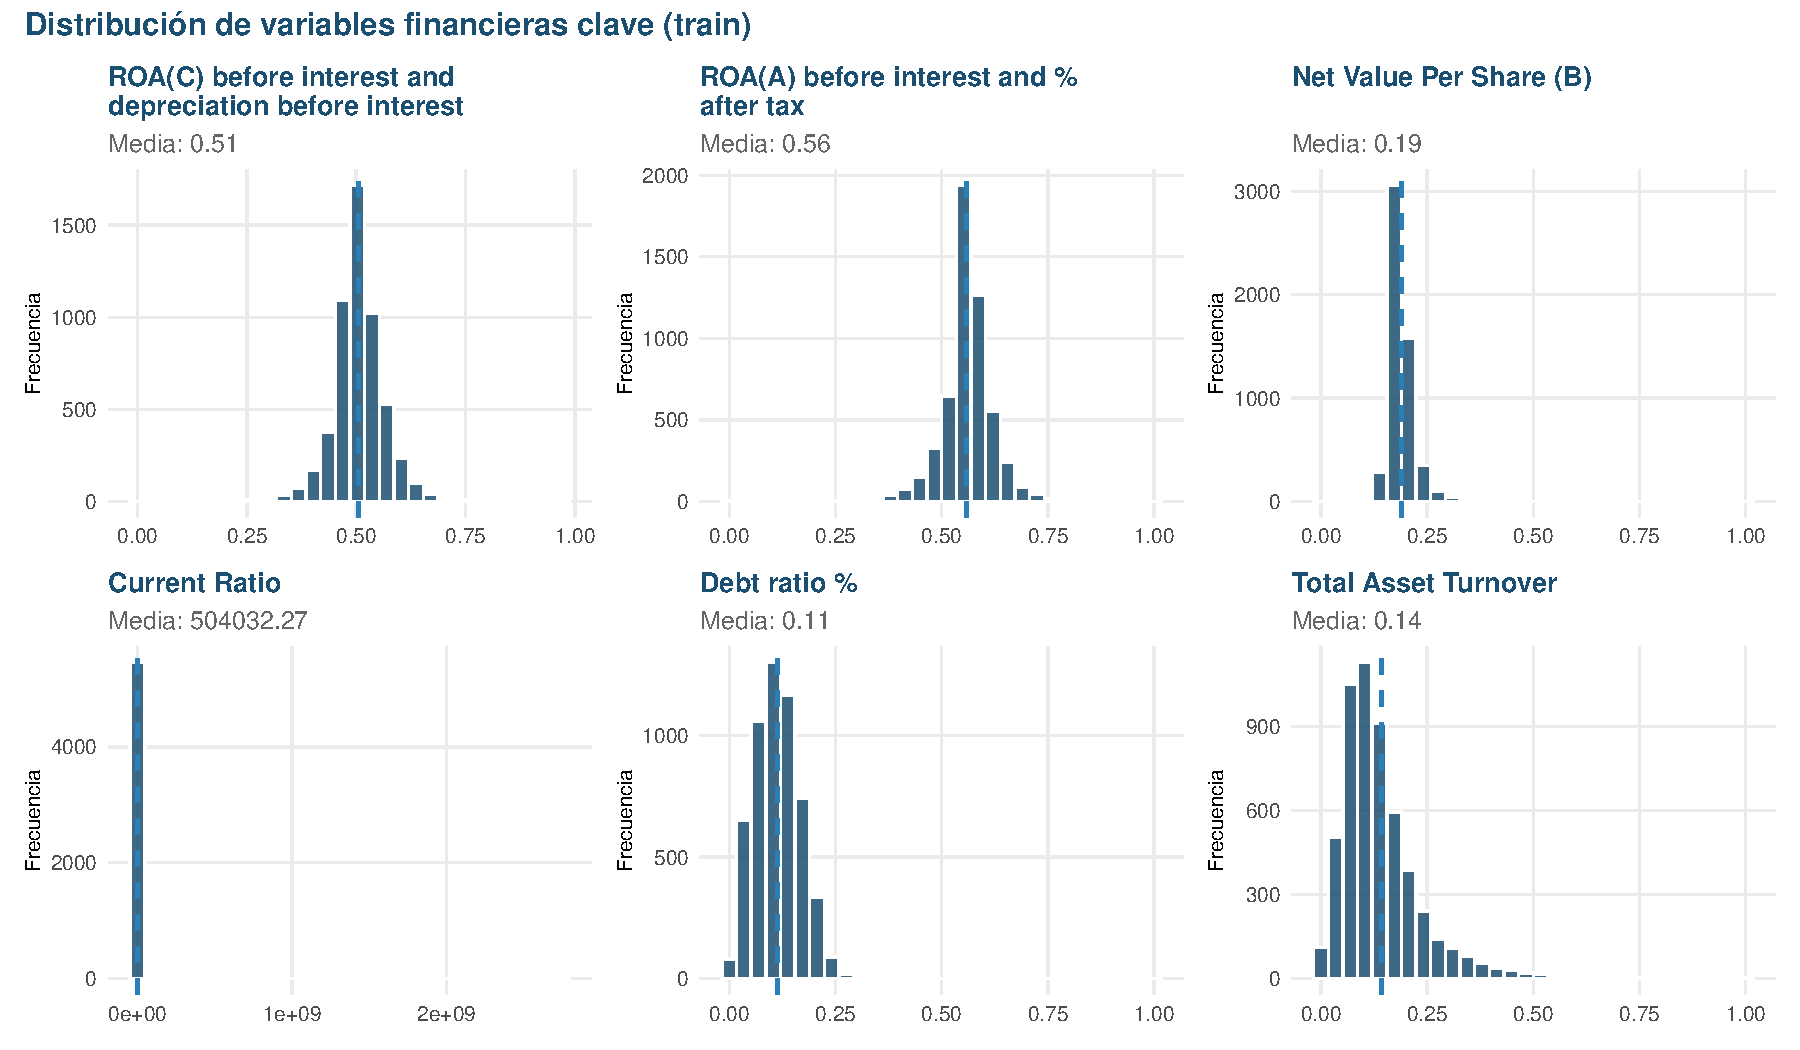
\includegraphics[keepaspectratio]{Prediccion_Bancarrota_Empresarial_files/Prediccion_Bancarrota_Empresarial_files/figure-latex/hist-clave-1.pdf}}

\begin{itemize}
\tightlist
\item
  \textbf{ROA(C) before interest and depreciation:} La mayoría de los valores se concentra
  alrededor de 0.5. La distribución presenta una ligera asimetría hacia la derecha y
  algunos valores alejados del centro.
\item
  \textbf{ROA(A) before interest and \% after tax:} La distribución también se concentra
  cerca de 0.55 y presenta una ligera asimetría hacia la derecha. Se observan algunos
  valores extremos en ambos lados, aunque la mayor parte de los datos se encuentra en
  un rango reducido.
\item
  \textbf{Net Value Per Share (B):} Los valores se concentran principalmente alrededor de
  0.18--0.20. La distribución está sesgada hacia la derecha, con una cola que se
  extiende hasta valores cercanos a 0.5.
\item
  \textbf{Current Ratio:} Presenta una fuerte asimetría hacia la derecha. La mayoría de las
  empresas tiene valores cercanos a 0, mientras que unas pocas presentan valores mucho
  más altos. Esto indica la presencia de valores extremos que podrían influir en
  algunos análisis estadísticos.
\item
  \textbf{Debt ratio \%:} La mayor parte de los valores se concentra aproximadamente entre
  0.05 y 0.20. La distribución presenta asimetría positiva, con una cola hacia valores
  más altos.
\item
  \textbf{Total Asset Turnover:} Los valores se concentran principalmente entre 0.05 y 0.20
  y la distribución está sesgada hacia la derecha. Hay algunas empresas con valores
  considerablemente mayores que la mayoría.
\end{itemize}

En general, las variables presentan distribuciones diferentes. Los indicadores Current
Ratio, Debt Ratio y Total Asset Turnover muestran una asimetría positiva más marcada y
posibles valores extremos. Estos casos deben revisarse en etapas posteriores antes de
decidir si requieren algún tratamiento.

\section{Distribución de la variable objetivo}\label{distribuciuxf3n-de-la-variable-objetivo}

\begin{Shaded}
\begin{Highlighting}[]
\NormalTok{conteo     }\OtherTok{\textless{}{-}} \FunctionTok{table}\NormalTok{(train\_df[[TARGET]])}
\NormalTok{porcentaje }\OtherTok{\textless{}{-}} \FunctionTok{prop.table}\NormalTok{(conteo) }\SpecialCharTok{*} \DecValTok{100}

\FunctionTok{cat}\NormalTok{(}\StringTok{"Total de empresas en train:"}\NormalTok{, }\FunctionTok{nrow}\NormalTok{(train\_df), }\StringTok{"}\SpecialCharTok{\textbackslash{}n}\StringTok{"}\NormalTok{)}
\end{Highlighting}
\end{Shaded}

\begin{verbatim}
## Total de empresas en train: 5456
\end{verbatim}

\begin{Shaded}
\begin{Highlighting}[]
\FunctionTok{cat}\NormalTok{(}\FunctionTok{sprintf}\NormalTok{(}\StringTok{"No quebradas (0): \%5d (\%.2f\%\%)}\SpecialCharTok{\textbackslash{}n}\StringTok{"}\NormalTok{, conteo[}\StringTok{"0"}\NormalTok{], porcentaje[}\StringTok{"0"}\NormalTok{]))}
\end{Highlighting}
\end{Shaded}

\begin{verbatim}
## No quebradas (0):  5269 (96.57%)
\end{verbatim}

\begin{Shaded}
\begin{Highlighting}[]
\FunctionTok{cat}\NormalTok{(}\FunctionTok{sprintf}\NormalTok{(}\StringTok{"Quebradas   (1): \%5d (\%.2f\%\%)}\SpecialCharTok{\textbackslash{}n}\StringTok{"}\NormalTok{, conteo[}\StringTok{"1"}\NormalTok{], porcentaje[}\StringTok{"1"}\NormalTok{]))}
\end{Highlighting}
\end{Shaded}

\begin{verbatim}
## Quebradas   (1):   187 (3.43%)
\end{verbatim}

\begin{Shaded}
\begin{Highlighting}[]
\FunctionTok{cat}\NormalTok{(}\FunctionTok{sprintf}\NormalTok{(}\StringTok{"Ratio de desbalance: \%.1f : 1}\SpecialCharTok{\textbackslash{}n}\StringTok{"}\NormalTok{, conteo[}\StringTok{"0"}\NormalTok{] }\SpecialCharTok{/}\NormalTok{ conteo[}\StringTok{"1"}\NormalTok{]))}
\end{Highlighting}
\end{Shaded}

\begin{verbatim}
## Ratio de desbalance: 28.2 : 1
\end{verbatim}

\begin{Shaded}
\begin{Highlighting}[]
\NormalTok{df\_plot }\OtherTok{\textless{}{-}} \FunctionTok{tibble}\NormalTok{(}\AttributeTok{clase =} \FunctionTok{names}\NormalTok{(conteo), }\AttributeTok{n =} \FunctionTok{as.numeric}\NormalTok{(conteo)) }\SpecialCharTok{\%\textgreater{}\%}
  \FunctionTok{mutate}\NormalTok{(}\AttributeTok{label =}\NormalTok{ TARGET\_LABELS[clase], }\AttributeTok{pct =}\NormalTok{ n }\SpecialCharTok{/} \FunctionTok{sum}\NormalTok{(n) }\SpecialCharTok{*} \DecValTok{100}\NormalTok{)}

\NormalTok{p\_barras }\OtherTok{\textless{}{-}} \FunctionTok{ggplot}\NormalTok{(df\_plot, }\FunctionTok{aes}\NormalTok{(}\AttributeTok{x =}\NormalTok{ label, }\AttributeTok{y =}\NormalTok{ n, }\AttributeTok{fill =}\NormalTok{ clase)) }\SpecialCharTok{+}
  \FunctionTok{geom\_col}\NormalTok{(}\AttributeTok{width =} \FloatTok{0.6}\NormalTok{) }\SpecialCharTok{+}
  \FunctionTok{geom\_text}\NormalTok{(}\FunctionTok{aes}\NormalTok{(}\AttributeTok{label =} \FunctionTok{sprintf}\NormalTok{(}\StringTok{"\%s}\SpecialCharTok{\textbackslash{}n}\StringTok{(\%.2f\%\%)"}\NormalTok{, }\FunctionTok{comma}\NormalTok{(n), pct)),}
            \AttributeTok{vjust =} \SpecialCharTok{{-}}\FloatTok{0.3}\NormalTok{, }\AttributeTok{fontface =} \StringTok{"bold"}\NormalTok{, }\AttributeTok{size =} \FloatTok{3.5}\NormalTok{) }\SpecialCharTok{+}
  \FunctionTok{scale\_fill\_manual}\NormalTok{(}\AttributeTok{values =}\NormalTok{ TARGET\_COLORS) }\SpecialCharTok{+}
  \FunctionTok{labs}\NormalTok{(}\AttributeTok{title =} \StringTok{"Conteo de empresas por clase (train)"}\NormalTok{, }\AttributeTok{x =} \ConstantTok{NULL}\NormalTok{,}
       \AttributeTok{y =} \StringTok{"Número de empresas"}\NormalTok{) }\SpecialCharTok{+}
  \FunctionTok{ylim}\NormalTok{(}\DecValTok{0}\NormalTok{, }\FunctionTok{max}\NormalTok{(df\_plot}\SpecialCharTok{$}\NormalTok{n) }\SpecialCharTok{*} \FloatTok{1.2}\NormalTok{) }\SpecialCharTok{+}
\NormalTok{  tema\_eda}

\NormalTok{p\_dona }\OtherTok{\textless{}{-}} \FunctionTok{ggplot}\NormalTok{(df\_plot, }\FunctionTok{aes}\NormalTok{(}\AttributeTok{x =} \DecValTok{2}\NormalTok{, }\AttributeTok{y =}\NormalTok{ pct, }\AttributeTok{fill =}\NormalTok{ clase)) }\SpecialCharTok{+}
  \FunctionTok{geom\_col}\NormalTok{(}\AttributeTok{color =} \StringTok{"white"}\NormalTok{, }\AttributeTok{linewidth =} \FloatTok{1.2}\NormalTok{) }\SpecialCharTok{+}
  \FunctionTok{coord\_polar}\NormalTok{(}\AttributeTok{theta =} \StringTok{"y"}\NormalTok{) }\SpecialCharTok{+}
  \FunctionTok{xlim}\NormalTok{(}\FloatTok{0.5}\NormalTok{, }\FloatTok{2.5}\NormalTok{) }\SpecialCharTok{+}
  \FunctionTok{scale\_fill\_manual}\NormalTok{(}\AttributeTok{values =}\NormalTok{ TARGET\_COLORS, }\AttributeTok{labels =}\NormalTok{ TARGET\_LABELS,}
                     \AttributeTok{name =} \ConstantTok{NULL}\NormalTok{) }\SpecialCharTok{+}
  \FunctionTok{geom\_text}\NormalTok{(}\FunctionTok{aes}\NormalTok{(}\AttributeTok{label =} \FunctionTok{sprintf}\NormalTok{(}\StringTok{"\%.2f\%\%"}\NormalTok{, pct)),}
            \AttributeTok{position =} \FunctionTok{position\_stack}\NormalTok{(}\AttributeTok{vjust =} \FloatTok{0.5}\NormalTok{), }\AttributeTok{color =} \StringTok{"white"}\NormalTok{,}
            \AttributeTok{fontface =} \StringTok{"bold"}\NormalTok{) }\SpecialCharTok{+}
  \FunctionTok{labs}\NormalTok{(}\AttributeTok{title =} \StringTok{"Proporción de empresas por clase (train)"}\NormalTok{) }\SpecialCharTok{+}
  \FunctionTok{theme\_void}\NormalTok{() }\SpecialCharTok{+}
  \FunctionTok{theme}\NormalTok{(}\AttributeTok{plot.title =} \FunctionTok{element\_text}\NormalTok{(}\AttributeTok{face =} \StringTok{"bold"}\NormalTok{, }\AttributeTok{size =} \DecValTok{13}\NormalTok{, }\AttributeTok{color =}\NormalTok{ COLOR\_MAIN,}
                                   \AttributeTok{hjust =} \FloatTok{0.5}\NormalTok{),}
        \AttributeTok{legend.position =} \StringTok{"right"}\NormalTok{)}

\NormalTok{p\_barras }\SpecialCharTok{+}\NormalTok{ p\_dona}
\end{Highlighting}
\end{Shaded}

\pandocbounded{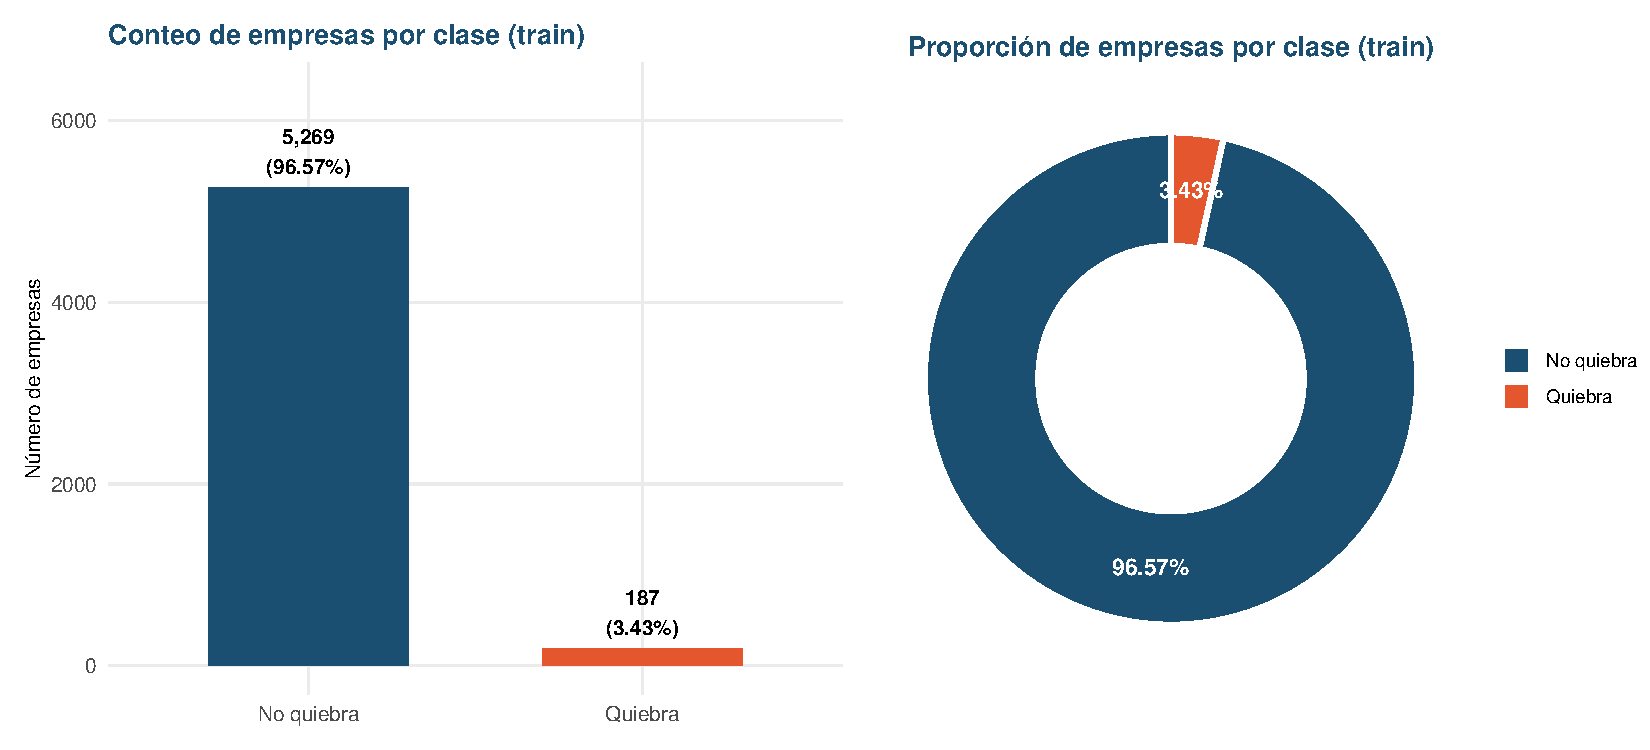
\includegraphics[keepaspectratio]{Prediccion_Bancarrota_Empresarial_files/Prediccion_Bancarrota_Empresarial_files/figure-latex/target-dist-1.pdf}}

\begin{quote}
\textbf{En palabras cortas:} La variable objetivo presenta un fuerte desbalance de
clases, ya que las empresas en quiebra representan solo el 3,23 \% del conjunto de
entrenamiento. Este desbalance deberá tenerse en cuenta durante el entrenamiento y
la evaluación del modelo.
\end{quote}

\chapter{\texorpdfstring{Análisis de outliers y sesgo (sobre \texttt{train})}{Análisis de outliers y sesgo (sobre train)}}\label{anuxe1lisis-de-outliers-y-sesgo-sobre-train}

Antes de pasar al análisis bivariado, es importante identificar qué variables tienen
distribuciones muy sesgadas y/o outliers extremos, ya que esto afecta tanto la
interpretación visual como la elección de modelos y transformaciones en la fase de
Machine Learning.

\section{Top 10 variables con mayor sesgo, en valor absoluto (train)}\label{top-10-variables-con-mayor-sesgo-en-valor-absoluto-train}

\begin{Shaded}
\begin{Highlighting}[]
\CommentTok{\# type = 2 replica la fórmula de sesgo "clásica" (similar a pandas .skew())}
\NormalTok{skew\_vals }\OtherTok{\textless{}{-}} \FunctionTok{sapply}\NormalTok{(train\_df[num\_vars], }\ControlFlowTok{function}\NormalTok{(x) e1071}\SpecialCharTok{::}\FunctionTok{skewness}\NormalTok{(x, }\AttributeTok{na.rm =} \ConstantTok{TRUE}\NormalTok{, }\AttributeTok{type =} \DecValTok{2}\NormalTok{))}
\NormalTok{skew\_orden }\OtherTok{\textless{}{-}} \FunctionTok{names}\NormalTok{(}\FunctionTok{sort}\NormalTok{(}\FunctionTok{abs}\NormalTok{(skew\_vals), }\AttributeTok{decreasing =} \ConstantTok{TRUE}\NormalTok{))}

\NormalTok{top10\_skew }\OtherTok{\textless{}{-}}\NormalTok{ skew\_vals[skew\_orden[}\DecValTok{1}\SpecialCharTok{:}\DecValTok{10}\NormalTok{]]}
\FunctionTok{print}\NormalTok{(}\FunctionTok{round}\NormalTok{(top10\_skew, }\DecValTok{2}\NormalTok{))}
\end{Highlighting}
\end{Shaded}

\begin{verbatim}
##                           Current Ratio                  Fixed Assets to Assets 
##                                   73.86                                   73.86 
##                   Net Value Growth Rate        Contingent liabilities/Net worth 
##                                   71.82                                   71.47 
## Realized Sales Gross Profit Growth Rate                   Operating Profit Rate 
##                                   69.87                                  -69.78 
##            Operating Profit Growth Rate                      Cash Flow to Sales 
##                                  -67.59                                  -65.51 
##          Working capitcal Turnover Rate             After-tax net Interest Rate 
##                                  -64.67                                  -61.97
\end{verbatim}

\begin{Shaded}
\begin{Highlighting}[]
\NormalTok{top\_skew\_vars }\OtherTok{\textless{}{-}}\NormalTok{ skew\_orden[}\DecValTok{1}\SpecialCharTok{:}\DecValTok{6}\NormalTok{]}
\end{Highlighting}
\end{Shaded}

Las variables presentan valores de sesgo muy altos, tanto positivos como negativos.
Esto indica que varias distribuciones están alejadas de una distribución simétrica y
pueden presentar valores extremos.

\textbf{Fixed Assets to Assets, Revenue per person} y \textbf{Net Value Growth Rate} presentan el
mayor sesgo positivo. Esto indica una fuerte concentración de los datos en ciertos
valores y la presencia de observaciones extremas hacia la derecha. \textbf{Operating Profit
Rate}, por su parte, suele presentar un sesgo negativo marcado, lo que indica una
distribución con una cola pronunciada hacia la izquierda. Otras variables como
\textbf{Contingent liabilities/Net worth} y \textbf{Working capital Turnover Rate} también
presentan valores de sesgo elevados.

\textbf{Conclusión:} Varias variables presentan un sesgo elevado, lo que sugiere la
presencia de distribuciones muy asimétricas y posibles valores extremos. Estas
variables deberán revisarse durante el preprocesamiento para determinar si requieren
alguna transformación, especialmente si se utilizan modelos sensibles a la escala o a
la distribución de los datos.

\section{Boxplots de las variables más sesgadas}\label{boxplots-de-las-variables-muxe1s-sesgadas}

\begin{Shaded}
\begin{Highlighting}[]
\NormalTok{plot\_box\_skew }\OtherTok{\textless{}{-}} \ControlFlowTok{function}\NormalTok{(var) \{}
  \FunctionTok{ggplot}\NormalTok{(train\_df, }\FunctionTok{aes}\NormalTok{(}\AttributeTok{x =} \StringTok{""}\NormalTok{, }\AttributeTok{y =}\NormalTok{ .data[[var]])) }\SpecialCharTok{+}
    \FunctionTok{geom\_boxplot}\NormalTok{(}\AttributeTok{fill =}\NormalTok{ COLOR\_MAIN, }\AttributeTok{color =}\NormalTok{ COLOR\_MAIN, }\AttributeTok{width =} \FloatTok{0.35}\NormalTok{,}
                 \AttributeTok{outlier.color =}\NormalTok{ COLOR\_RISK, }\AttributeTok{outlier.alpha =} \FloatTok{0.5}\NormalTok{, }\AttributeTok{outlier.size =} \FloatTok{1.5}\NormalTok{) }\SpecialCharTok{+}
    \FunctionTok{labs}\NormalTok{(}\AttributeTok{title =} \FunctionTok{sprintf}\NormalTok{(}\StringTok{"\%s}\SpecialCharTok{\textbackslash{}n}\StringTok{(skew = \%.1f)"}\NormalTok{, }\FunctionTok{str\_wrap}\NormalTok{(var, }\DecValTok{28}\NormalTok{), skew\_vals[var]),}
         \AttributeTok{x =} \ConstantTok{NULL}\NormalTok{, }\AttributeTok{y =} \ConstantTok{NULL}\NormalTok{) }\SpecialCharTok{+}
\NormalTok{    tema\_eda}
\NormalTok{\}}

\FunctionTok{wrap\_plots}\NormalTok{(}\FunctionTok{lapply}\NormalTok{(top\_skew\_vars, plot\_box\_skew), }\AttributeTok{ncol =} \DecValTok{3}\NormalTok{) }\SpecialCharTok{+}
  \FunctionTok{plot\_annotation}\NormalTok{(}\AttributeTok{title =} \StringTok{"Variables con mayor sesgo (train)"}\NormalTok{,}
                   \AttributeTok{theme =} \FunctionTok{theme}\NormalTok{(}\AttributeTok{plot.title =} \FunctionTok{element\_text}\NormalTok{(}\AttributeTok{face =} \StringTok{"bold"}\NormalTok{, }\AttributeTok{size =} \DecValTok{15}\NormalTok{)))}
\end{Highlighting}
\end{Shaded}

\pandocbounded{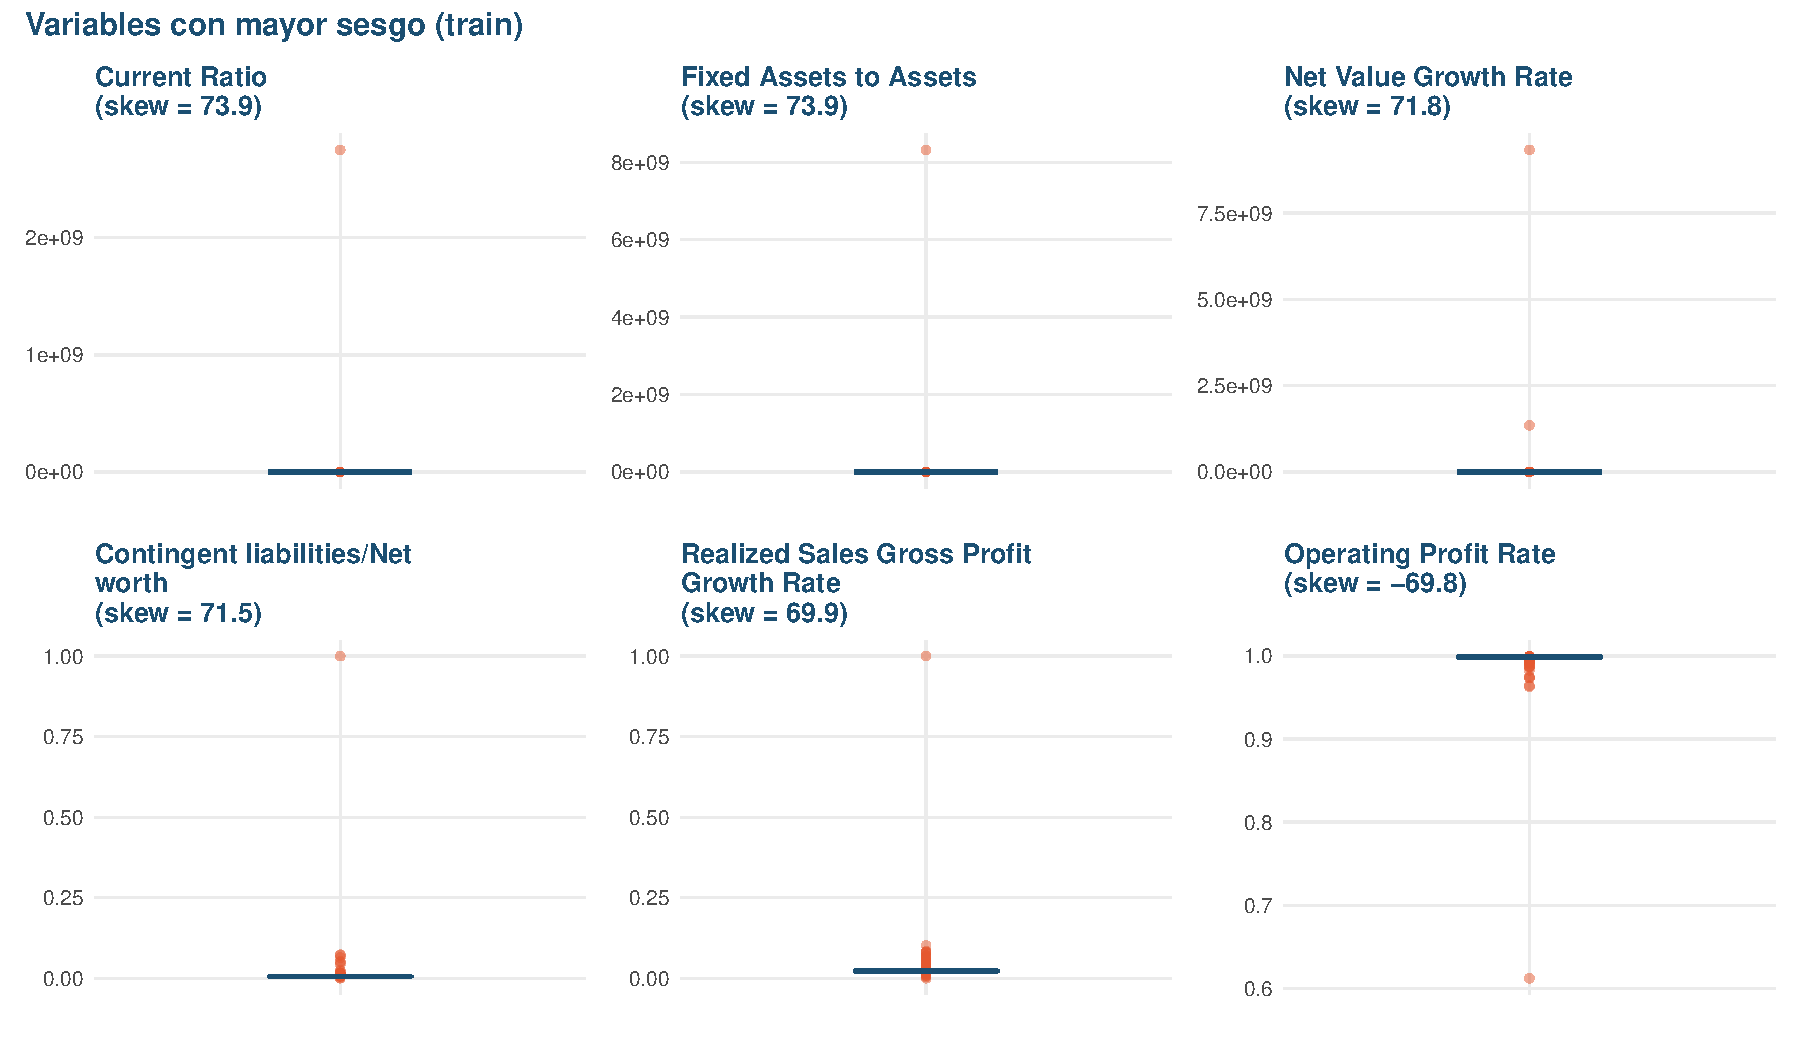
\includegraphics[keepaspectratio]{Prediccion_Bancarrota_Empresarial_files/Prediccion_Bancarrota_Empresarial_files/figure-latex/box-sesgo-1.pdf}}

\begin{itemize}
\tightlist
\item
  \textbf{Fixed Assets to Assets:} La mayoría de los valores se concentra cerca de cero,
  pero aparece un valor extremadamente alto. Esto explica el fuerte sesgo positivo y
  muestra la presencia de un valor atípico muy marcado.
\item
  \textbf{Revenue per person:} Presenta un comportamiento similar. La mayoría de las
  observaciones está concentrada en valores bajos, mientras que existe un valor
  extremadamente alto que distorsiona la distribución.
\item
  \textbf{Net Value Growth Rate:} Casi todos los valores se encuentran cerca de cero, pero
  se observa un valor muy alejado del resto. Este valor extremo explica gran parte del
  sesgo positivo de la variable.
\item
  \textbf{Total income/Total expense:} La mayoría de las observaciones se concentra cerca
  de valores bajos, mientras que aparece un valor cercano a 1 claramente separado del
  resto. Esto indica una distribución muy asimétrica y la presencia de un posible
  valor atípico.
\item
  \textbf{Operating Profit Rate:} Los valores están muy concentrados cerca de 1, aunque
  aparecen algunas observaciones alejadas, principalmente hacia valores inferiores.
  Esto genera el fuerte sesgo negativo observado anteriormente.
\item
  \textbf{Contingent liabilities/Net worth:} La mayoría de los datos se encuentra cerca de
  cero, pero aparecen varios valores alejados y uno cercano a 1. Estos valores
  extremos contribuyen al elevado sesgo positivo.
\end{itemize}

\textbf{Conclusión:} Los boxplots muestran que las variables con mayor sesgo presentan
valores atípicos muy alejados de la mayoría de las observaciones. En varias de ellas,
estos valores extremos explican gran parte del sesgo observado. Por ahora no se
deberían eliminar automáticamente, ya que primero es necesario determinar si
representan errores o situaciones reales de las empresas.

\section{Top 15 variables con más outliers (regla IQR)}\label{top-15-variables-con-muxe1s-outliers-regla-iqr}

\begin{Shaded}
\begin{Highlighting}[]
\NormalTok{pct\_outliers\_iqr }\OtherTok{\textless{}{-}} \ControlFlowTok{function}\NormalTok{(x) \{}
\NormalTok{  q   }\OtherTok{\textless{}{-}} \FunctionTok{quantile}\NormalTok{(x, }\FunctionTok{c}\NormalTok{(}\FloatTok{0.25}\NormalTok{, }\FloatTok{0.75}\NormalTok{), }\AttributeTok{na.rm =} \ConstantTok{TRUE}\NormalTok{)}
\NormalTok{  iqr }\OtherTok{\textless{}{-}}\NormalTok{ q[}\DecValTok{2}\NormalTok{] }\SpecialCharTok{{-}}\NormalTok{ q[}\DecValTok{1}\NormalTok{]}
\NormalTok{  lower }\OtherTok{\textless{}{-}}\NormalTok{ q[}\DecValTok{1}\NormalTok{] }\SpecialCharTok{{-}} \FloatTok{1.5} \SpecialCharTok{*}\NormalTok{ iqr}
\NormalTok{  upper }\OtherTok{\textless{}{-}}\NormalTok{ q[}\DecValTok{2}\NormalTok{] }\SpecialCharTok{+} \FloatTok{1.5} \SpecialCharTok{*}\NormalTok{ iqr}
  \FunctionTok{mean}\NormalTok{(x }\SpecialCharTok{\textless{}}\NormalTok{ lower }\SpecialCharTok{|}\NormalTok{ x }\SpecialCharTok{\textgreater{}}\NormalTok{ upper, }\AttributeTok{na.rm =} \ConstantTok{TRUE}\NormalTok{) }\SpecialCharTok{*} \DecValTok{100}
\NormalTok{\}}

\NormalTok{outlier\_pct }\OtherTok{\textless{}{-}} \FunctionTok{sort}\NormalTok{(}\FunctionTok{sapply}\NormalTok{(train\_df[num\_vars], pct\_outliers\_iqr), }\AttributeTok{decreasing =} \ConstantTok{TRUE}\NormalTok{)}
\NormalTok{top15\_out   }\OtherTok{\textless{}{-}}\NormalTok{ outlier\_pct[}\DecValTok{1}\SpecialCharTok{:}\DecValTok{15}\NormalTok{]}
\FunctionTok{print}\NormalTok{(}\FunctionTok{round}\NormalTok{(top15\_out, }\DecValTok{1}\NormalTok{))}
\end{Highlighting}
\end{Shaded}

\begin{verbatim}
##                 Degree of Financial Leverage (DFL) 
##                                               22.2 
##                    Fixed Assets Turnover Frequency 
##                                               20.8 
## Interest Coverage Ratio (Interest expense to EBIT) 
##                                               20.7 
##                        Current Asset Turnover Rate 
##                                               20.6 
##                            Total Asset Growth Rate 
##                                               20.1 
##                             Interest Expense Ratio 
##                                               19.2 
##                             Cash Flow to Liability 
##                                               18.1 
##                                 No-credit Interval 
##                                               16.4 
##        Non-industry income and expenditure/revenue 
##                                               16.1 
##                                 Cash Flow to Sales 
##                                               15.5 
##                       Operating Profit Growth Rate 
##                                               15.3 
##                  Continuous Net Profit Growth Rate 
##                                               15.3 
##                   After-tax Net Profit Growth Rate 
##                                               15.2 
##                     Regular Net Profit Growth Rate 
##                                               15.2 
##                          Inventory/Working Capital 
##                                               13.9
\end{verbatim}

\begin{Shaded}
\begin{Highlighting}[]
\NormalTok{df\_out }\OtherTok{\textless{}{-}} \FunctionTok{tibble}\NormalTok{(}\AttributeTok{variable =} \FunctionTok{names}\NormalTok{(top15\_out), }\AttributeTok{pct =} \FunctionTok{as.numeric}\NormalTok{(top15\_out))}

\FunctionTok{ggplot}\NormalTok{(df\_out, }\FunctionTok{aes}\NormalTok{(}\AttributeTok{x =} \FunctionTok{reorder}\NormalTok{(variable, pct), }\AttributeTok{y =}\NormalTok{ pct)) }\SpecialCharTok{+}
  \FunctionTok{geom\_col}\NormalTok{(}\AttributeTok{fill =}\NormalTok{ COLOR\_MAIN) }\SpecialCharTok{+}
  \FunctionTok{geom\_text}\NormalTok{(}\FunctionTok{aes}\NormalTok{(}\AttributeTok{label =} \FunctionTok{sprintf}\NormalTok{(}\StringTok{"\%.1f\%\%"}\NormalTok{, pct)), }\AttributeTok{hjust =} \SpecialCharTok{{-}}\FloatTok{0.15}\NormalTok{, }\AttributeTok{size =} \FloatTok{3.2}\NormalTok{,}
            \AttributeTok{color =}\NormalTok{ COLOR\_MAIN, }\AttributeTok{fontface =} \StringTok{"bold"}\NormalTok{) }\SpecialCharTok{+}
  \FunctionTok{coord\_flip}\NormalTok{(}\AttributeTok{clip =} \StringTok{"off"}\NormalTok{) }\SpecialCharTok{+}
  \FunctionTok{labs}\NormalTok{(}\AttributeTok{title =} \StringTok{"Top 15 variables con más outliers (IQR, train)"}\NormalTok{,}
       \AttributeTok{x =} \ConstantTok{NULL}\NormalTok{, }\AttributeTok{y =} \StringTok{"\% de empresas marcadas como outlier"}\NormalTok{) }\SpecialCharTok{+}
  \FunctionTok{expand\_limits}\NormalTok{(}\AttributeTok{y =} \FunctionTok{max}\NormalTok{(df\_out}\SpecialCharTok{$}\NormalTok{pct) }\SpecialCharTok{*} \FloatTok{1.15}\NormalTok{) }\SpecialCharTok{+}
\NormalTok{  tema\_eda}
\end{Highlighting}
\end{Shaded}

\pandocbounded{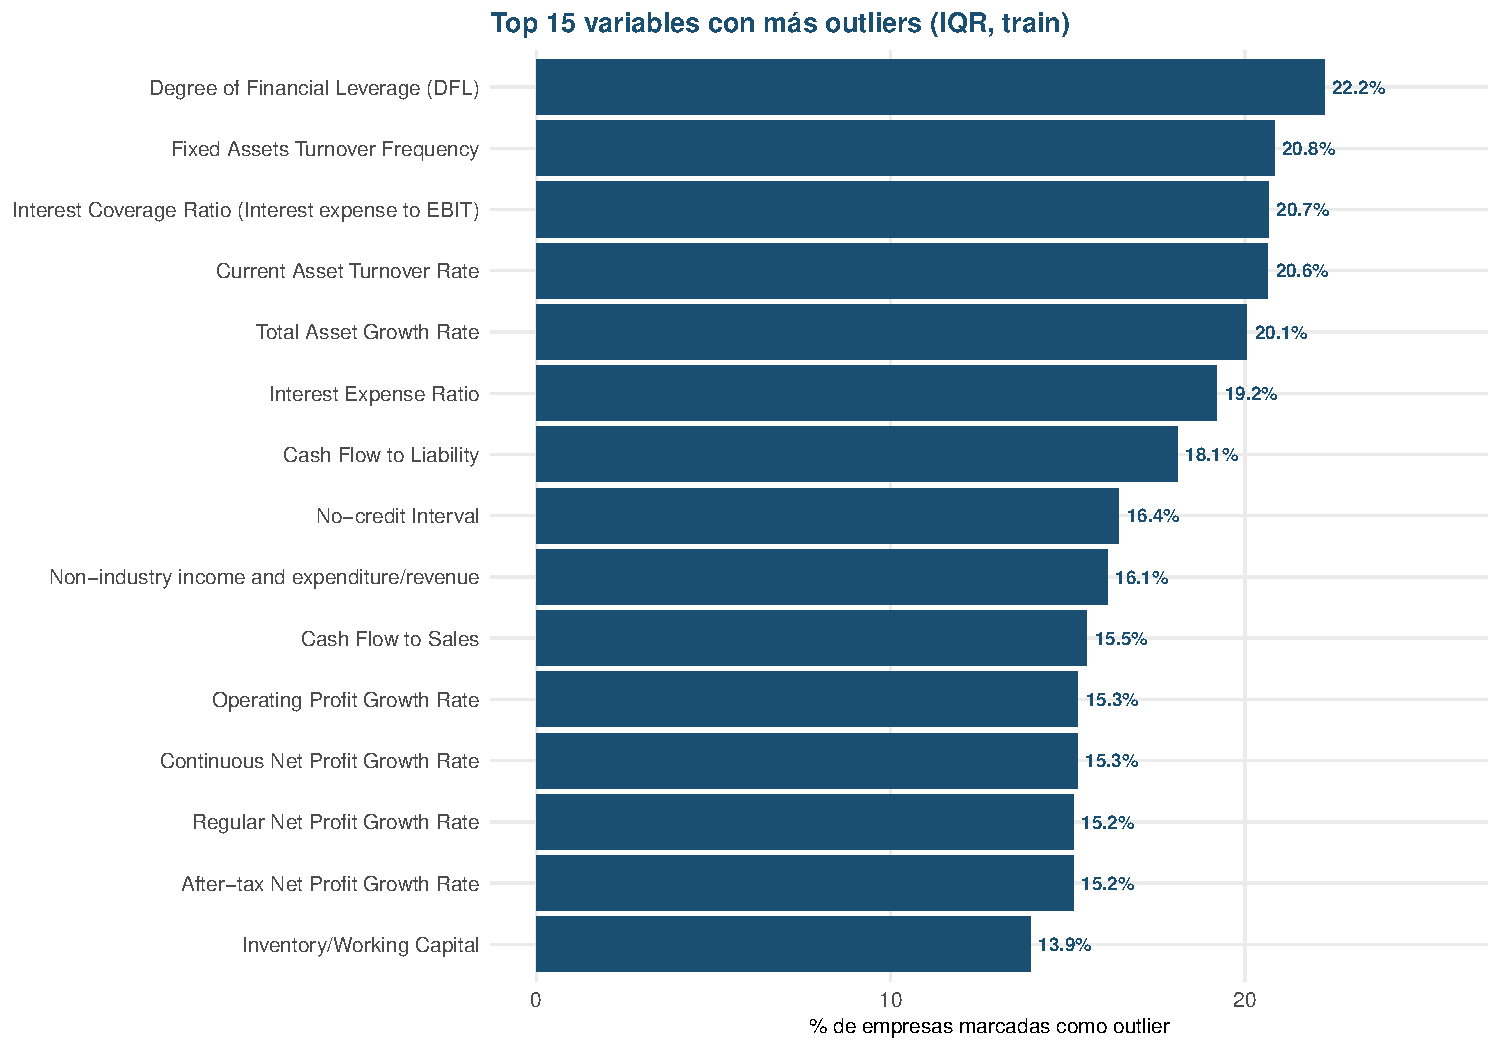
\includegraphics[keepaspectratio]{Prediccion_Bancarrota_Empresarial_files/Prediccion_Bancarrota_Empresarial_files/figure-latex/outliers-iqr-1.pdf}}

Las variables con mayor proporción de valores atípicos suelen ser \textbf{Degree of
Financial Leverage (DFL)}, \textbf{Fixed Assets Turnover Frequency} e \textbf{Interest Coverage
Ratio}, con alrededor del 20 \% de empresas marcadas como outliers. También destacan
\textbf{Current Asset Turnover Rate}, \textbf{Total Asset Growth Rate} e \textbf{Interest Expense
Ratio}, con porcentajes similares. Las demás variables del top 15 presentan entre
aproximadamente 14 \% y 18 \% de observaciones marcadas como outliers.

En general, varias variables presentan una proporción considerable de valores
atípicos. Sin embargo, esto no significa que deban eliminarse automáticamente, ya que
pueden representar situaciones financieras reales de algunas empresas. Estos
resultados deberán considerarse posteriormente al definir el preprocesamiento de los
datos.

\chapter{\texorpdfstring{Análisis bivariado: variables vs.~objetivo (sobre \texttt{train})}{Análisis bivariado: variables vs.~objetivo (sobre train)}}\label{anuxe1lisis-bivariado-variables-vs.-objetivo-sobre-train}

\section{Variables más importantes según Random Forest}\label{variables-muxe1s-importantes-seguxfan-random-forest}

Usamos un Random Forest \textbf{entrenado únicamente con \texttt{train}} para tener una primera
idea de qué variables separan mejor a las empresas que quiebran de las que no. Esto es
solo exploratorio: nos ayuda a elegir qué variables mirar con más detalle en los
gráficos siguientes, no es el modelo final del proyecto.

\begin{quote}
\textbf{¿Por qué Random Forest?} Se eligió porque no necesita que las variables estén en
la misma escala ni sigan una relación lineal con la quiebra, es robusto ante los
outliers que ya se identificaron en los datos y entrega una medida de importancia de
variables por defecto, facilitando la interpretación para fines exploratorios.
\end{quote}

\begin{Shaded}
\begin{Highlighting}[]
\CommentTok{\# Nota metodológica: la imputación con la mediana que se hace aquí es temporal y}
\CommentTok{\# solo existe para poder entrenar el Random Forest exploratorio; no se aplica a}
\CommentTok{\# train\_df ni al dataset real. La imputación definitiva se decide en la etapa de}
\CommentTok{\# preprocesamiento, después del EDA.}

\NormalTok{X\_rf }\OtherTok{\textless{}{-}}\NormalTok{ train\_df }\SpecialCharTok{\%\textgreater{}\%} \FunctionTok{select}\NormalTok{(}\SpecialCharTok{{-}}\FunctionTok{all\_of}\NormalTok{(TARGET), }\SpecialCharTok{{-}}\StringTok{\textasciigrave{}}\AttributeTok{Net Income Flag}\StringTok{\textasciigrave{}}\NormalTok{)}

\NormalTok{X\_rf }\OtherTok{\textless{}{-}}\NormalTok{ X\_rf }\SpecialCharTok{\%\textgreater{}\%}
  \FunctionTok{mutate}\NormalTok{(}\FunctionTok{across}\NormalTok{(}\FunctionTok{everything}\NormalTok{(), }\SpecialCharTok{\textasciitilde{}} \FunctionTok{ifelse}\NormalTok{(}\FunctionTok{is.infinite}\NormalTok{(.x), }\ConstantTok{NA}\NormalTok{, .x))) }\SpecialCharTok{\%\textgreater{}\%}
  \FunctionTok{mutate}\NormalTok{(}\FunctionTok{across}\NormalTok{(}\FunctionTok{everything}\NormalTok{(), }\SpecialCharTok{\textasciitilde{}} \FunctionTok{ifelse}\NormalTok{(}\FunctionTok{is.na}\NormalTok{(.x), }\FunctionTok{median}\NormalTok{(.x, }\AttributeTok{na.rm =} \ConstantTok{TRUE}\NormalTok{), .x)))}

\NormalTok{y\_train\_factor }\OtherTok{\textless{}{-}} \FunctionTok{factor}\NormalTok{(train\_df[[TARGET]], }\AttributeTok{levels =} \FunctionTok{c}\NormalTok{(}\DecValTok{0}\NormalTok{, }\DecValTok{1}\NormalTok{),}
                          \AttributeTok{labels =} \FunctionTok{c}\NormalTok{(}\StringTok{"No"}\NormalTok{, }\StringTok{"Si"}\NormalTok{))}

\FunctionTok{set.seed}\NormalTok{(RANDOM\_STATE)}
\NormalTok{rf }\OtherTok{\textless{}{-}} \FunctionTok{randomForest}\NormalTok{(}\AttributeTok{x =}\NormalTok{ X\_rf, }\AttributeTok{y =}\NormalTok{ y\_train\_factor, }\AttributeTok{ntree =} \DecValTok{100}\NormalTok{, }\AttributeTok{importance =} \ConstantTok{TRUE}\NormalTok{)}

\CommentTok{\# MeanDecreaseGini es el equivalente conceptual a feature\_importances\_ de sklearn}
\NormalTok{importancias }\OtherTok{\textless{}{-}} \FunctionTok{importance}\NormalTok{(rf, }\AttributeTok{type =} \DecValTok{2}\NormalTok{)[, }\DecValTok{1}\NormalTok{]}
\NormalTok{importancias }\OtherTok{\textless{}{-}} \FunctionTok{sort}\NormalTok{(importancias, }\AttributeTok{decreasing =} \ConstantTok{TRUE}\NormalTok{)}

\FunctionTok{cat}\NormalTok{(}\StringTok{"============================================================}\SpecialCharTok{\textbackslash{}n}\StringTok{"}\NormalTok{)}
\end{Highlighting}
\end{Shaded}

\begin{verbatim}
## ============================================================
\end{verbatim}

\begin{Shaded}
\begin{Highlighting}[]
\FunctionTok{cat}\NormalTok{(}\StringTok{"TOP 15 VARIABLES MÁS IMPORTANTES (Random Forest, train)}\SpecialCharTok{\textbackslash{}n}\StringTok{"}\NormalTok{)}
\end{Highlighting}
\end{Shaded}

\begin{verbatim}
## TOP 15 VARIABLES MÁS IMPORTANTES (Random Forest, train)
\end{verbatim}

\begin{Shaded}
\begin{Highlighting}[]
\FunctionTok{cat}\NormalTok{(}\StringTok{"============================================================}\SpecialCharTok{\textbackslash{}n}\StringTok{"}\NormalTok{)}
\end{Highlighting}
\end{Shaded}

\begin{verbatim}
## ============================================================
\end{verbatim}

\begin{Shaded}
\begin{Highlighting}[]
\FunctionTok{print}\NormalTok{(}\FunctionTok{round}\NormalTok{(}\FunctionTok{head}\NormalTok{(importancias, }\DecValTok{15}\NormalTok{), }\DecValTok{3}\NormalTok{))}
\end{Highlighting}
\end{Shaded}

\begin{verbatim}
##                              Net Value Growth Rate 
##                                             13.636 
##            Persistent EPS in the Last Four Seasons 
##                                             10.215 
##                 Net Income to Stockholder's Equity 
##                                             10.044 
##                               Borrowing dependency 
##                                              9.609 
##              Net profit before tax/Paid-in capital 
##                                              8.345 
##                             Working Capital/Equity 
##                                              7.247 
##                 Degree of Financial Leverage (DFL) 
##                                              7.012 
##                Interest-bearing debt interest rate 
##                                              7.011 
##                         Total debt/Total net worth 
##                                              6.903 
##                            Net Value Per Share (B) 
##                                              6.826 
##           Per Share Net profit before tax (Yuan ¥) 
##                                              6.398 
##        Non-industry income and expenditure/revenue 
##                                              6.305 
##                                Equity to Liability 
##                                              5.830 
##                    Working Capital to Total Assets 
##                                              5.650 
## Interest Coverage Ratio (Interest expense to EBIT) 
##                                              5.610
\end{verbatim}

\begin{Shaded}
\begin{Highlighting}[]
\NormalTok{top\_15\_features }\OtherTok{\textless{}{-}} \FunctionTok{names}\NormalTok{(}\FunctionTok{head}\NormalTok{(importancias, }\DecValTok{15}\NormalTok{))}
\NormalTok{top\_6\_features  }\OtherTok{\textless{}{-}} \FunctionTok{names}\NormalTok{(}\FunctionTok{head}\NormalTok{(importancias, }\DecValTok{6}\NormalTok{))}

\NormalTok{df\_imp }\OtherTok{\textless{}{-}} \FunctionTok{tibble}\NormalTok{(}\AttributeTok{variable =} \FunctionTok{names}\NormalTok{(}\FunctionTok{head}\NormalTok{(importancias, }\DecValTok{15}\NormalTok{)),}
                  \AttributeTok{importancia =} \FunctionTok{as.numeric}\NormalTok{(}\FunctionTok{head}\NormalTok{(importancias, }\DecValTok{15}\NormalTok{))) }\SpecialCharTok{\%\textgreater{}\%}
  \FunctionTok{mutate}\NormalTok{(}\AttributeTok{top6 =}\NormalTok{ variable }\SpecialCharTok{\%in\%}\NormalTok{ top\_6\_features)}

\FunctionTok{ggplot}\NormalTok{(df\_imp, }\FunctionTok{aes}\NormalTok{(}\AttributeTok{x =} \FunctionTok{reorder}\NormalTok{(variable, importancia), }\AttributeTok{y =}\NormalTok{ importancia, }\AttributeTok{fill =}\NormalTok{ top6)) }\SpecialCharTok{+}
  \FunctionTok{geom\_col}\NormalTok{() }\SpecialCharTok{+}
  \FunctionTok{geom\_text}\NormalTok{(}\FunctionTok{aes}\NormalTok{(}\AttributeTok{label =} \FunctionTok{sprintf}\NormalTok{(}\StringTok{"\%.3f"}\NormalTok{, importancia)), }\AttributeTok{hjust =} \SpecialCharTok{{-}}\FloatTok{0.15}\NormalTok{, }\AttributeTok{size =} \DecValTok{3}\NormalTok{,}
            \AttributeTok{fontface =} \StringTok{"bold"}\NormalTok{, }\AttributeTok{color =}\NormalTok{ COLOR\_MAIN) }\SpecialCharTok{+}
  \FunctionTok{coord\_flip}\NormalTok{(}\AttributeTok{clip =} \StringTok{"off"}\NormalTok{) }\SpecialCharTok{+}
  \FunctionTok{scale\_fill\_manual}\NormalTok{(}\AttributeTok{values =} \FunctionTok{c}\NormalTok{(}\StringTok{\textasciigrave{}}\AttributeTok{TRUE}\StringTok{\textasciigrave{}} \OtherTok{=}\NormalTok{ COLOR\_RISK, }\StringTok{\textasciigrave{}}\AttributeTok{FALSE}\StringTok{\textasciigrave{}} \OtherTok{=}\NormalTok{ COLOR\_MAIN),}
                     \AttributeTok{labels =} \FunctionTok{c}\NormalTok{(}\StringTok{\textasciigrave{}}\AttributeTok{TRUE}\StringTok{\textasciigrave{}} \OtherTok{=} \StringTok{"Top 6 (usadas más abajo)"}\NormalTok{,}
                                \StringTok{\textasciigrave{}}\AttributeTok{FALSE}\StringTok{\textasciigrave{}} \OtherTok{=} \StringTok{"Resto del top 15"}\NormalTok{),}
                     \AttributeTok{name =} \ConstantTok{NULL}\NormalTok{) }\SpecialCharTok{+}
  \FunctionTok{labs}\NormalTok{(}\AttributeTok{title =} \StringTok{"Top 15 variables más importantes}\SpecialCharTok{\textbackslash{}n}\StringTok{(Random Forest sobre train)"}\NormalTok{,}
       \AttributeTok{x =} \ConstantTok{NULL}\NormalTok{, }\AttributeTok{y =} \StringTok{"Importancia (MeanDecreaseGini)"}\NormalTok{) }\SpecialCharTok{+}
  \FunctionTok{expand\_limits}\NormalTok{(}\AttributeTok{y =} \FunctionTok{max}\NormalTok{(df\_imp}\SpecialCharTok{$}\NormalTok{importancia) }\SpecialCharTok{*} \FloatTok{1.2}\NormalTok{) }\SpecialCharTok{+}
\NormalTok{  tema\_eda }\SpecialCharTok{+}
  \FunctionTok{theme}\NormalTok{(}\AttributeTok{legend.position =} \StringTok{"bottom"}\NormalTok{)}
\end{Highlighting}
\end{Shaded}

\pandocbounded{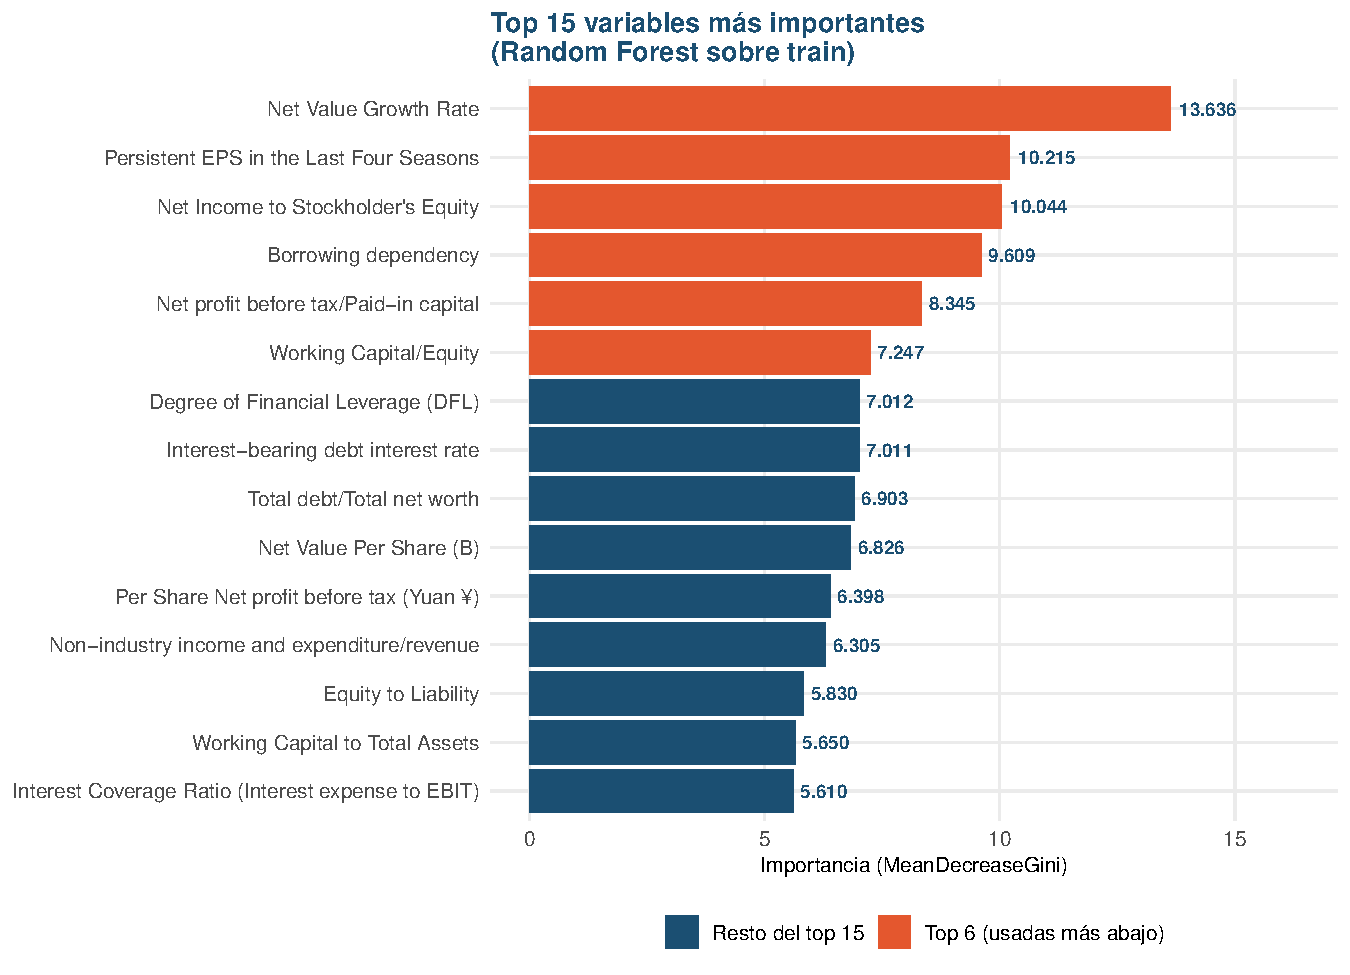
\includegraphics[keepaspectratio]{Prediccion_Bancarrota_Empresarial_files/Prediccion_Bancarrota_Empresarial_files/figure-latex/rf-importancia-1.pdf}}

\begin{quote}
\textbf{¿Qué hizo Random Forest aquí?} Es un modelo que, al entrenarse, mide qué tanto le
``ayudó'' cada variable para diferenciar empresas que quiebran de las que no. Cuanto
mayor el número de importancia, más útil fue esa variable para el modelo. Entre las
más importantes suelen aparecer variables de rentabilidad para el accionista (\texttt{Net\ Income\ to\ Stockholder\textquotesingle{}s\ Equity}), márgenes operativos y ratios de endeudamiento ---
lo cual tiene sentido: una empresa que no genera ganancias para sus dueños y está
muy endeudada es, intuitivamente, más propensa a quebrar.
\end{quote}

Random Forest se utiliza aquí como una \textbf{herramienta exploratoria}, no como un
ranking definitivo de importancia. Dos sesgos conocidos a tener en cuenta:

\begin{itemize}
\tightlist
\item
  \textbf{Favorece variables continuas sobre categóricas:} una variable binaria como
  \texttt{Liability-Assets\ Flag} casi nunca aparecerá entre las ``más importantes'', aunque sí
  sea relevante.
\item
  \textbf{Reparte la importancia entre variables correlacionadas:} cuando varias variables
  miden algo muy parecido (como las distintas versiones de ROA), el modelo divide el
  ``crédito'' entre ellas, lo que puede subestimar su relevancia individual.
\end{itemize}

\section{Variables más importantes vs.~objetivo}\label{variables-muxe1s-importantes-vs.-objetivo}

\begin{Shaded}
\begin{Highlighting}[]
\NormalTok{plot\_box\_target }\OtherTok{\textless{}{-}} \ControlFlowTok{function}\NormalTok{(var) \{}
\NormalTok{  q1  }\OtherTok{\textless{}{-}} \FunctionTok{quantile}\NormalTok{(train\_df[[var]], }\FloatTok{0.01}\NormalTok{, }\AttributeTok{na.rm =} \ConstantTok{TRUE}\NormalTok{)}
\NormalTok{  q99 }\OtherTok{\textless{}{-}} \FunctionTok{quantile}\NormalTok{(train\_df[[var]], }\FloatTok{0.99}\NormalTok{, }\AttributeTok{na.rm =} \ConstantTok{TRUE}\NormalTok{)}
\NormalTok{  df\_f }\OtherTok{\textless{}{-}}\NormalTok{ train\_df }\SpecialCharTok{\%\textgreater{}\%} \FunctionTok{filter}\NormalTok{(.data[[var]] }\SpecialCharTok{\textgreater{}=}\NormalTok{ q1, .data[[var]] }\SpecialCharTok{\textless{}=}\NormalTok{ q99)}

  \FunctionTok{ggplot}\NormalTok{(df\_f, }\FunctionTok{aes}\NormalTok{(}\AttributeTok{x =} \FunctionTok{as.factor}\NormalTok{(.data[[TARGET]]), }\AttributeTok{y =}\NormalTok{ .data[[var]],}
                    \AttributeTok{fill =} \FunctionTok{as.factor}\NormalTok{(.data[[TARGET]]))) }\SpecialCharTok{+}
    \FunctionTok{geom\_boxplot}\NormalTok{(}\AttributeTok{width =} \FloatTok{0.45}\NormalTok{, }\AttributeTok{outlier.alpha =} \FloatTok{0.35}\NormalTok{, }\AttributeTok{outlier.size =} \FloatTok{1.2}\NormalTok{) }\SpecialCharTok{+}
    \FunctionTok{scale\_x\_discrete}\NormalTok{(}\AttributeTok{labels =}\NormalTok{ TARGET\_LABELS) }\SpecialCharTok{+}
    \FunctionTok{scale\_fill\_manual}\NormalTok{(}\AttributeTok{values =}\NormalTok{ TARGET\_COLORS) }\SpecialCharTok{+}
    \FunctionTok{labs}\NormalTok{(}\AttributeTok{title =} \FunctionTok{str\_wrap}\NormalTok{(var, }\DecValTok{32}\NormalTok{), }\AttributeTok{x =} \ConstantTok{NULL}\NormalTok{, }\AttributeTok{y =}\NormalTok{ var) }\SpecialCharTok{+}
\NormalTok{    tema\_eda}
\NormalTok{\}}

\FunctionTok{wrap\_plots}\NormalTok{(}\FunctionTok{lapply}\NormalTok{(top\_6\_features, plot\_box\_target), }\AttributeTok{ncol =} \DecValTok{3}\NormalTok{) }\SpecialCharTok{+}
  \FunctionTok{plot\_annotation}\NormalTok{(}
    \AttributeTok{title =} \StringTok{"Variables más importantes vs. objetivo}\SpecialCharTok{\textbackslash{}n}\StringTok{(train, sin el 1\% de valores más extremos)"}\NormalTok{,}
    \AttributeTok{theme =} \FunctionTok{theme}\NormalTok{(}\AttributeTok{plot.title =} \FunctionTok{element\_text}\NormalTok{(}\AttributeTok{face =} \StringTok{"bold"}\NormalTok{, }\AttributeTok{size =} \DecValTok{15}\NormalTok{))}
\NormalTok{  )}
\end{Highlighting}
\end{Shaded}

\pandocbounded{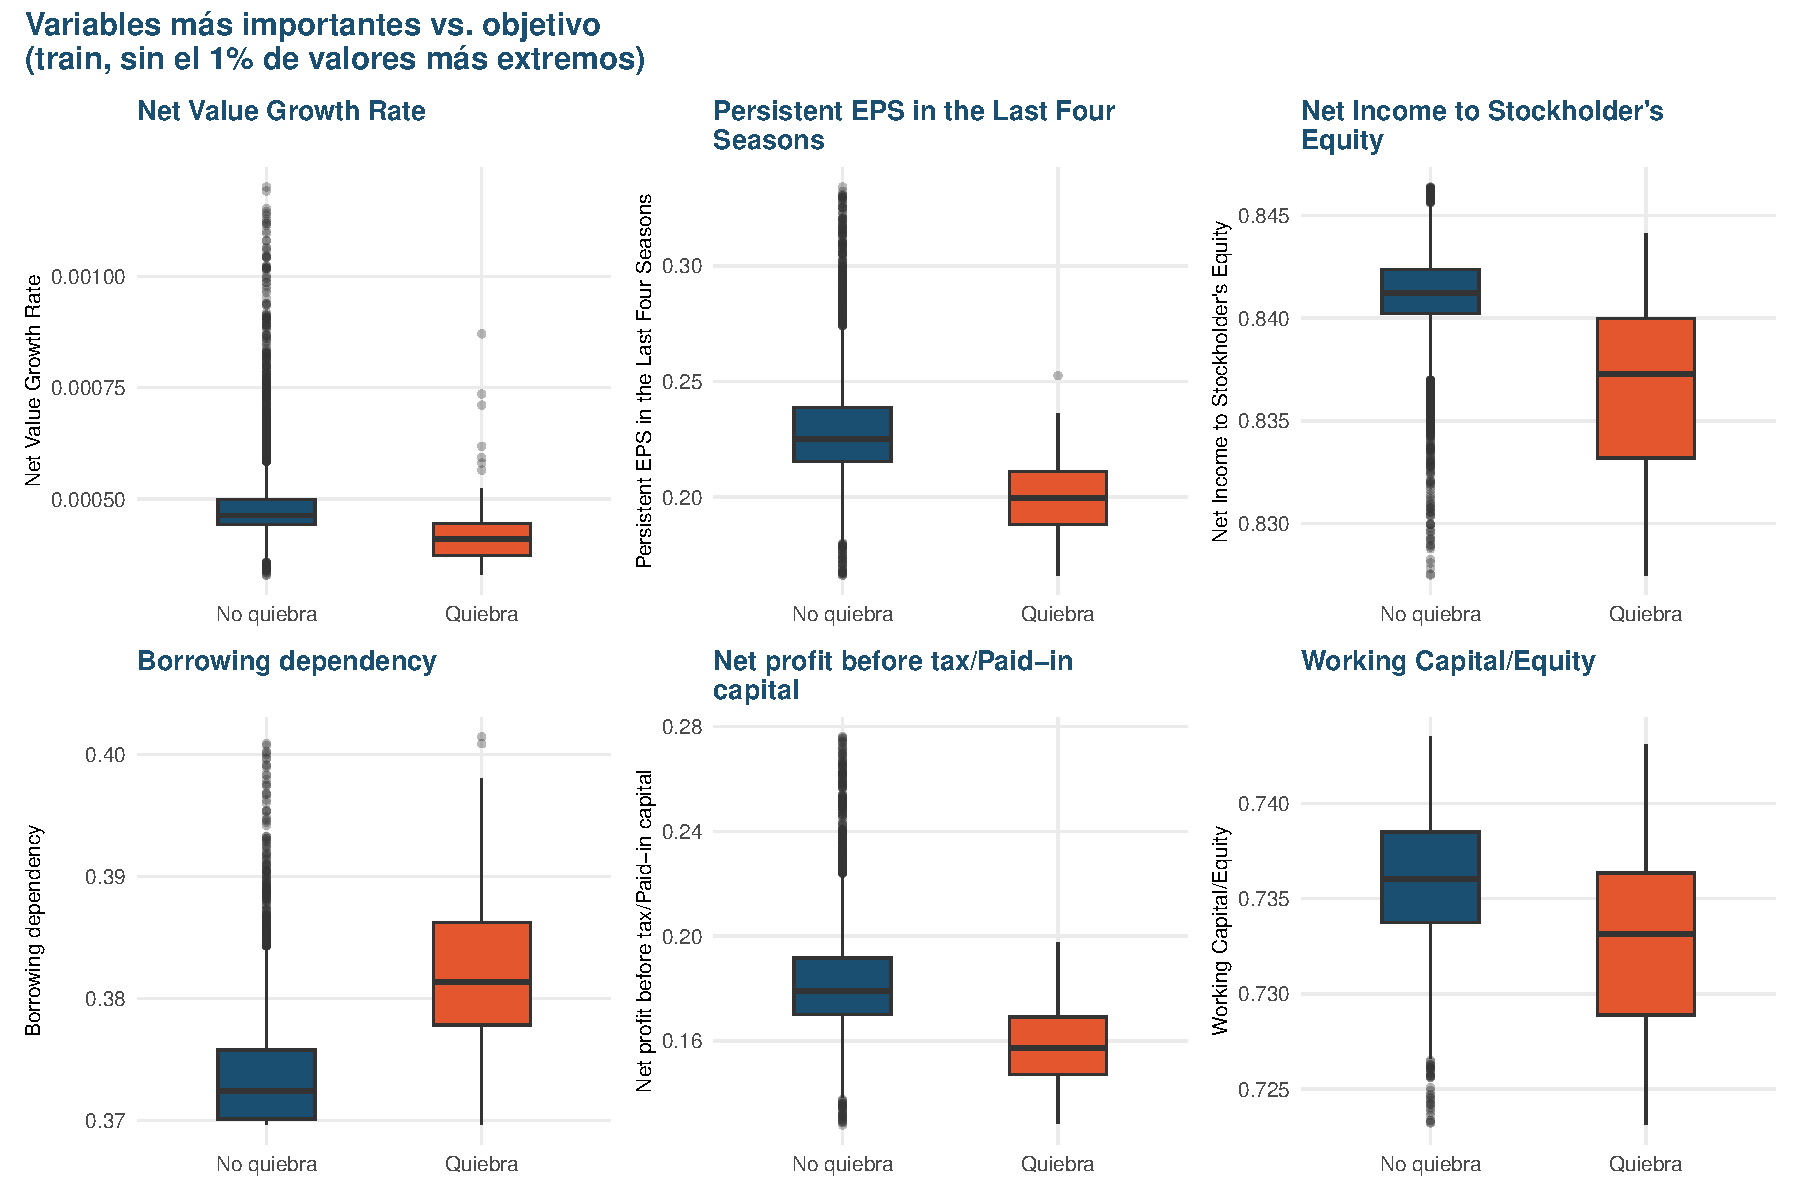
\includegraphics[keepaspectratio]{Prediccion_Bancarrota_Empresarial_files/Prediccion_Bancarrota_Empresarial_files/figure-latex/box-top6-1.pdf}}

Estos boxplots comparan la distribución de cada variable entre empresas que
quebraron y que no, y muestran patrones distintos según el tipo de variable:

\begin{itemize}
\tightlist
\item
  \textbf{Variables de rentabilidad} (\texttt{Net\ Income\ to\ Stockholder\textquotesingle{}s\ Equity}, \texttt{Persistent\ EPS\ in\ the\ Last\ Four\ Seasons}, \texttt{Net\ profit\ before\ tax/Paid-in\ capital}): en las tres, el
  grupo que \textbf{quebró tiene medianas más bajas y cajas más dispersas} (sobre todo \texttt{Net\ Income\ to\ Stockholder\textquotesingle{}s\ Equity}, donde la caja de ``Quiebra'' es mucho más ancha).
  Esto confirma que las empresas que quiebran tienden a ser menos rentables, y de
  forma menos homogénea --- hay más variedad de situaciones dentro de ese grupo.
\item
  \textbf{\texttt{Borrowing\ dependency}:} suele ser el panel con la separación más clara --- el
  grupo ``Quiebra'' tiene una mediana notablemente más alta y su caja casi no se
  superpone con la de ``No quiebra''. Confirma, en la práctica, lo que ya muestra la
  correlación más adelante: mayor dependencia de financiamiento externo se asocia con
  mayor riesgo de quiebra.
\item
  \textbf{\texttt{Net\ Value\ Growth\ Rate} e \texttt{Interest\ Expense\ Ratio}:} aquí la diferencia entre
  grupos suele ser mínima --- las cajas se superponen bastante y las medianas están muy
  cerca. Son variables que el Random Forest consideró relevantes en conjunto con las
  demás, pero que por sí solas, vistas de forma aislada, no separan claramente a las
  empresas que quiebran.
\end{itemize}

En conjunto, el patrón refuerza lo que se venía viendo en la sección: \textbf{rentabilidad
baja y endeudamiento alto son las señales más visibles de riesgo}, mientras que otras
variables importantes para el modelo probablemente aportan valor más por su
interacción con las demás que por separarse solas en un boxplot.

\emph{Nota: dependiendo de la partición \texttt{train}/\texttt{test} que te haya tocado, es posible que
el orden exacto de las 6 variables top varíe un poco respecto a esta descripción ---
ajusta los nombres si es necesario.}

\section{\texorpdfstring{\texttt{Liability-Assets\ Flag} vs.~objetivo}{Liability-Assets Flag vs.~objetivo}}\label{liability-assets-flag-vs.-objetivo}

Análisis bivariado de la única variable categórica con la variable objetivo.

\textbf{\texttt{Liability-Assets\ Flag}:} es la única variable categórica del dataset. Es binaria e
indica si los pasivos de la empresa superan a sus activos (\texttt{1}) o no (\texttt{0}).

\begin{Shaded}
\begin{Highlighting}[]
\NormalTok{tabla\_pct    }\OtherTok{\textless{}{-}} \FunctionTok{prop.table}\NormalTok{(}\FunctionTok{table}\NormalTok{(train\_df}\SpecialCharTok{$}\StringTok{\textasciigrave{}}\AttributeTok{Liability{-}Assets Flag}\StringTok{\textasciigrave{}}\NormalTok{, train\_df[[TARGET]]),}
                            \AttributeTok{margin =} \DecValTok{1}\NormalTok{) }\SpecialCharTok{*} \DecValTok{100}
\NormalTok{tabla\_conteo }\OtherTok{\textless{}{-}} \FunctionTok{table}\NormalTok{(train\_df}\SpecialCharTok{$}\StringTok{\textasciigrave{}}\AttributeTok{Liability{-}Assets Flag}\StringTok{\textasciigrave{}}\NormalTok{, train\_df[[TARGET]])}
\NormalTok{totales      }\OtherTok{\textless{}{-}} \FunctionTok{rowSums}\NormalTok{(tabla\_conteo)}

\FunctionTok{print}\NormalTok{(}\FunctionTok{round}\NormalTok{(tabla\_pct, }\DecValTok{2}\NormalTok{))}
\end{Highlighting}
\end{Shaded}

\begin{verbatim}
##    
##         0     1
##   0 96.66  3.34
##   1 28.57 71.43
\end{verbatim}

\begin{Shaded}
\begin{Highlighting}[]
\NormalTok{df\_flag }\OtherTok{\textless{}{-}} \FunctionTok{tibble}\NormalTok{(}
  \AttributeTok{flag   =} \FunctionTok{rownames}\NormalTok{(tabla\_pct),}
  \AttributeTok{pct\_quiebra =}\NormalTok{ tabla\_pct[, }\StringTok{"1"}\NormalTok{],}
  \AttributeTok{n      =} \FunctionTok{as.numeric}\NormalTok{(totales)}
\NormalTok{) }\SpecialCharTok{\%\textgreater{}\%}
  \FunctionTok{mutate}\NormalTok{(}\AttributeTok{etiqueta =} \FunctionTok{ifelse}\NormalTok{(flag }\SpecialCharTok{==} \StringTok{"0"}\NormalTok{,}
                            \StringTok{"Flag = 0}\SpecialCharTok{\textbackslash{}n}\StringTok{Activos \textgreater{} Pasivos (normal)"}\NormalTok{,}
                            \StringTok{"Flag = 1}\SpecialCharTok{\textbackslash{}n}\StringTok{Pasivos \textgreater{} Activos (alarma)"}\NormalTok{))}

\FunctionTok{ggplot}\NormalTok{(df\_flag, }\FunctionTok{aes}\NormalTok{(}\AttributeTok{x =}\NormalTok{ etiqueta, }\AttributeTok{y =}\NormalTok{ pct\_quiebra, }\AttributeTok{fill =}\NormalTok{ etiqueta)) }\SpecialCharTok{+}
  \FunctionTok{geom\_col}\NormalTok{(}\AttributeTok{width =} \FloatTok{0.5}\NormalTok{) }\SpecialCharTok{+}
  \FunctionTok{geom\_text}\NormalTok{(}\FunctionTok{aes}\NormalTok{(}\AttributeTok{label =} \FunctionTok{sprintf}\NormalTok{(}\StringTok{"\%.1f\%\% quebró}\SpecialCharTok{\textbackslash{}n}\StringTok{(n=\%d)"}\NormalTok{, pct\_quiebra, n)),}
            \AttributeTok{vjust =} \SpecialCharTok{{-}}\FloatTok{0.2}\NormalTok{, }\AttributeTok{fontface =} \StringTok{"bold"}\NormalTok{, }\AttributeTok{size =} \FloatTok{3.8}\NormalTok{) }\SpecialCharTok{+}
  \FunctionTok{scale\_fill\_manual}\NormalTok{(}\AttributeTok{values =} \FunctionTok{c}\NormalTok{(COLOR\_MAIN, COLOR\_RISK)) }\SpecialCharTok{+}
  \FunctionTok{labs}\NormalTok{(}\AttributeTok{title =} \StringTok{"¿El Liability{-}Assets Flag anticipa la quiebra?"}\NormalTok{,}
       \AttributeTok{x =} \ConstantTok{NULL}\NormalTok{, }\AttributeTok{y =} \StringTok{"\% de empresas del grupo que quebró"}\NormalTok{) }\SpecialCharTok{+}
  \FunctionTok{ylim}\NormalTok{(}\DecValTok{0}\NormalTok{, }\FunctionTok{max}\NormalTok{(df\_flag}\SpecialCharTok{$}\NormalTok{pct\_quiebra) }\SpecialCharTok{*} \FloatTok{1.3}\NormalTok{) }\SpecialCharTok{+}
\NormalTok{  tema\_eda}
\end{Highlighting}
\end{Shaded}

\pandocbounded{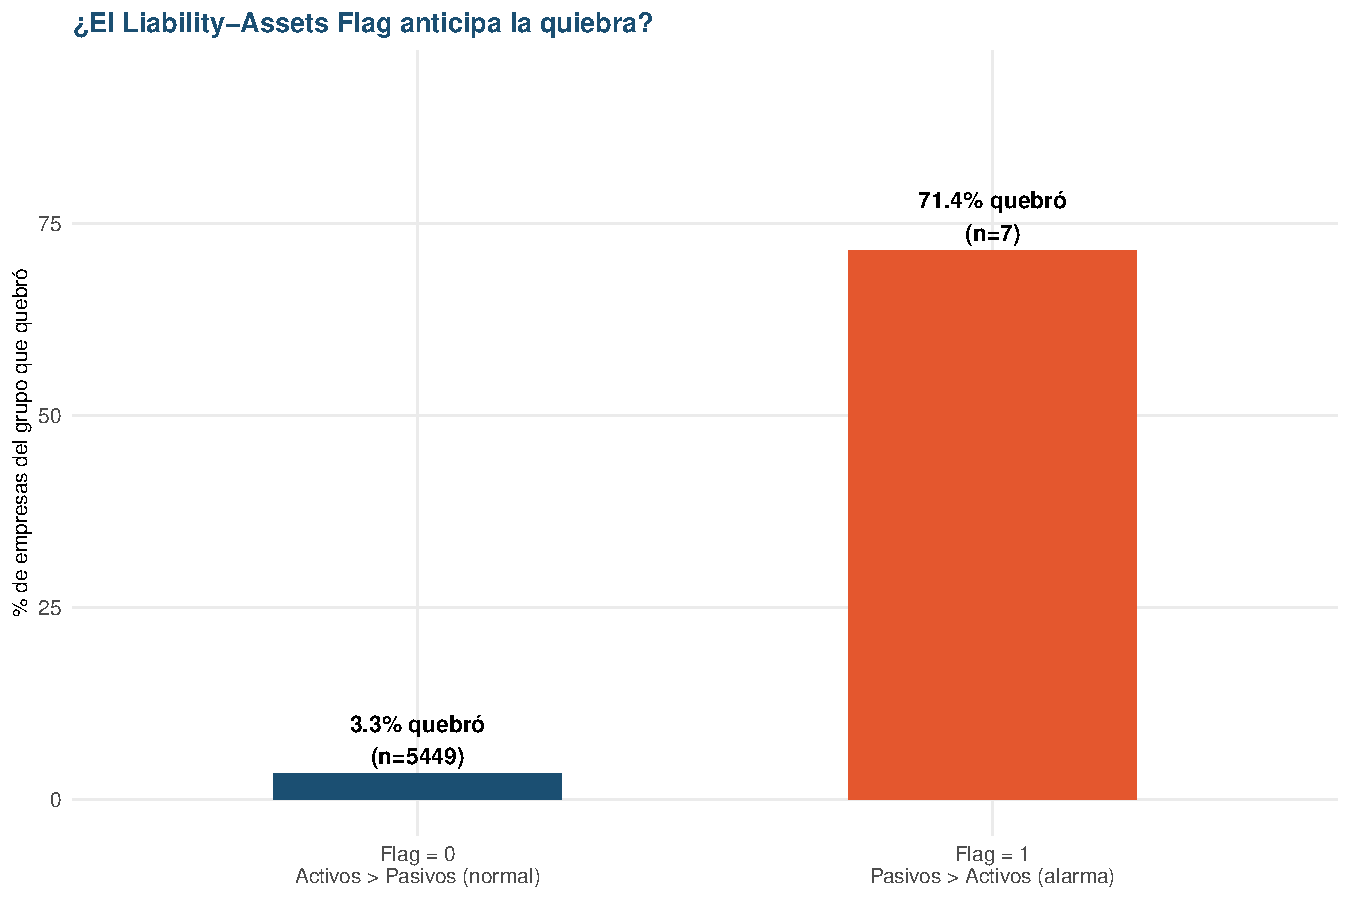
\includegraphics[keepaspectratio]{Prediccion_Bancarrota_Empresarial_files/Prediccion_Bancarrota_Empresarial_files/figure-latex/flag-vs-target-1.pdf}}

\emph{Alternativa fiel al gráfico de ``waffle'' (cuadrícula 10x10) del notebook original: si
quieres reproducirlo exactamente, instala el paquete \texttt{waffle}
(\texttt{install.packages("waffle")}) y usa \texttt{waffle::waffle()} sobre \texttt{tabla\_pct}.}

El grupo con \texttt{Flag\ =\ 1} (pasivos mayores que activos) suele tener una tasa de quiebra
dramáticamente más alta que el grupo \texttt{Flag\ =\ 0}. Es decir, cuando una empresa debe más
de lo que tiene, la probabilidad de que quiebre aumenta muchísimo.

Sin embargo, hay que leer este resultado con cautela: el grupo \texttt{Flag\ =\ 1} tiene muy
pocas empresas en \texttt{train} (revisa el \texttt{n} impreso arriba). Con una muestra tan pequeña,
el porcentaje es muy sensible a cualquier empresa individual y no es estadísticamente
robusto --- no podemos concluir con confianza que la relación sea tan fuerte en la
población general, aunque la dirección (más pasivos que activos → más riesgo) sí
tiene sentido financiero.

Por eso, aunque \texttt{Liability-Assets\ Flag} parece ser una señal de alerta útil, conviene
tratarla con precaución en el modelado: puede aportar información valiosa para ese
pequeño grupo de riesgo, pero su bajo número de casos limita qué tan bien puede
generalizar.

\section{Correlaciones con la variable objetivo}\label{correlaciones-con-la-variable-objetivo}

\begin{Shaded}
\begin{Highlighting}[]
\NormalTok{corr\_objetivo }\OtherTok{\textless{}{-}} \FunctionTok{sapply}\NormalTok{(train\_df[num\_vars], }\ControlFlowTok{function}\NormalTok{(x) \{}
  \FunctionTok{cor}\NormalTok{(x, train\_df[[TARGET]], }\AttributeTok{use =} \StringTok{"pairwise.complete.obs"}\NormalTok{)}
\NormalTok{\})}
\NormalTok{corr\_objetivo }\OtherTok{\textless{}{-}} \FunctionTok{sort}\NormalTok{(corr\_objetivo)}

\FunctionTok{cat}\NormalTok{(}\StringTok{"======================================================================}\SpecialCharTok{\textbackslash{}n}\StringTok{"}\NormalTok{)}
\end{Highlighting}
\end{Shaded}

\begin{verbatim}
## ======================================================================
\end{verbatim}

\begin{Shaded}
\begin{Highlighting}[]
\FunctionTok{cat}\NormalTok{(}\StringTok{"CORRELACIONES CON LA VARIABLE OBJETIVO, Bankrupt? (train)}\SpecialCharTok{\textbackslash{}n}\StringTok{"}\NormalTok{)}
\end{Highlighting}
\end{Shaded}

\begin{verbatim}
## CORRELACIONES CON LA VARIABLE OBJETIVO, Bankrupt? (train)
\end{verbatim}

\begin{Shaded}
\begin{Highlighting}[]
\FunctionTok{cat}\NormalTok{(}\StringTok{"======================================================================}\SpecialCharTok{\textbackslash{}n}\StringTok{"}\NormalTok{)}
\end{Highlighting}
\end{Shaded}

\begin{verbatim}
## ======================================================================
\end{verbatim}

\begin{Shaded}
\begin{Highlighting}[]
\FunctionTok{cat}\NormalTok{(}\StringTok{"}\SpecialCharTok{\textbackslash{}n}\StringTok{TOP 10 CORRELACIONES NEGATIVAS (más fuertes):}\SpecialCharTok{\textbackslash{}n}\StringTok{"}\NormalTok{)}
\end{Highlighting}
\end{Shaded}

\begin{verbatim}
## 
## TOP 10 CORRELACIONES NEGATIVAS (más fuertes):
\end{verbatim}

\begin{Shaded}
\begin{Highlighting}[]
\FunctionTok{print}\NormalTok{(}\FunctionTok{round}\NormalTok{(}\FunctionTok{head}\NormalTok{(corr\_objetivo, }\DecValTok{10}\NormalTok{), }\DecValTok{3}\NormalTok{))}
\end{Highlighting}
\end{Shaded}

\begin{verbatim}
##                              Net Income to Total Assets 
##                                                  -0.316 
##                  ROA(A) before interest and % after tax 
##                                                  -0.288 
##       ROA(B) before interest and depreciation after tax 
##                                                  -0.277 
## ROA(C) before interest and depreciation before interest 
##                                                  -0.267 
##                                        Net worth/Assets 
##                                                  -0.262 
##                 Persistent EPS in the Last Four Seasons 
##                                                  -0.230 
##                   Net profit before tax/Paid-in capital 
##                                                  -0.223 
##                Per Share Net profit before tax (Yuan ¥) 
##                                                  -0.214 
##                         Working Capital to Total Assets 
##                                                  -0.209 
##                       Retained Earnings to Total Assets 
##                                                  -0.207
\end{verbatim}

\begin{Shaded}
\begin{Highlighting}[]
\FunctionTok{cat}\NormalTok{(}\StringTok{"}\SpecialCharTok{\textbackslash{}n}\StringTok{TOP 10 CORRELACIONES POSITIVAS (más fuertes):}\SpecialCharTok{\textbackslash{}n}\StringTok{"}\NormalTok{)}
\end{Highlighting}
\end{Shaded}

\begin{verbatim}
## 
## TOP 10 CORRELACIONES POSITIVAS (más fuertes):
\end{verbatim}

\begin{Shaded}
\begin{Highlighting}[]
\FunctionTok{print}\NormalTok{(}\FunctionTok{round}\NormalTok{(}\FunctionTok{tail}\NormalTok{(corr\_objetivo, }\DecValTok{10}\NormalTok{), }\DecValTok{3}\NormalTok{))}
\end{Highlighting}
\end{Shaded}

\begin{verbatim}
## Inventory and accounts receivable/Net value 
##                                       0.098 
##                        Total expense/Assets 
##                                       0.134 
##                  Current Liabilities/Equity 
##                                       0.169 
##                 Current Liability to Equity 
##                                       0.169 
##               Equity to Long-term Liability 
##                                       0.180 
##                         Liability to Equity 
##                                       0.188 
##         Current Liability to Current Assets 
##                                       0.194 
##                 Current Liability to Assets 
##                                       0.197 
##                        Borrowing dependency 
##                                       0.207 
##                                Debt ratio % 
##                                       0.262
\end{verbatim}

\begin{Shaded}
\begin{Highlighting}[]
\NormalTok{top\_corr }\OtherTok{\textless{}{-}} \FunctionTok{c}\NormalTok{(}\FunctionTok{head}\NormalTok{(corr\_objetivo, }\DecValTok{10}\NormalTok{), }\FunctionTok{tail}\NormalTok{(corr\_objetivo, }\DecValTok{10}\NormalTok{))}
\NormalTok{df\_corr }\OtherTok{\textless{}{-}} \FunctionTok{tibble}\NormalTok{(}\AttributeTok{variable =} \FunctionTok{names}\NormalTok{(top\_corr), }\AttributeTok{valor =} \FunctionTok{as.numeric}\NormalTok{(top\_corr)) }\SpecialCharTok{\%\textgreater{}\%}
  \FunctionTok{mutate}\NormalTok{(}\AttributeTok{signo =} \FunctionTok{ifelse}\NormalTok{(valor }\SpecialCharTok{\textless{}} \DecValTok{0}\NormalTok{, }\StringTok{"Negativa"}\NormalTok{, }\StringTok{"Positiva"}\NormalTok{))}

\FunctionTok{ggplot}\NormalTok{(df\_corr, }\FunctionTok{aes}\NormalTok{(}\AttributeTok{x =} \FunctionTok{reorder}\NormalTok{(variable, valor), }\AttributeTok{y =}\NormalTok{ valor, }\AttributeTok{fill =}\NormalTok{ signo)) }\SpecialCharTok{+}
  \FunctionTok{geom\_col}\NormalTok{(}\AttributeTok{width =} \FloatTok{0.7}\NormalTok{) }\SpecialCharTok{+}
  \FunctionTok{geom\_text}\NormalTok{(}\FunctionTok{aes}\NormalTok{(}\AttributeTok{label =} \FunctionTok{sprintf}\NormalTok{(}\StringTok{"\%.2f"}\NormalTok{, valor),}
                \AttributeTok{hjust =} \FunctionTok{ifelse}\NormalTok{(valor }\SpecialCharTok{\textgreater{}=} \DecValTok{0}\NormalTok{, }\SpecialCharTok{{-}}\FloatTok{0.15}\NormalTok{, }\FloatTok{1.15}\NormalTok{)),}
            \AttributeTok{size =} \DecValTok{3}\NormalTok{, }\AttributeTok{color =} \StringTok{"grey30"}\NormalTok{) }\SpecialCharTok{+}
  \FunctionTok{geom\_hline}\NormalTok{(}\AttributeTok{yintercept =} \DecValTok{0}\NormalTok{, }\AttributeTok{color =} \StringTok{"grey40"}\NormalTok{) }\SpecialCharTok{+}
  \FunctionTok{coord\_flip}\NormalTok{(}\AttributeTok{clip =} \StringTok{"off"}\NormalTok{) }\SpecialCharTok{+}
  \FunctionTok{scale\_fill\_manual}\NormalTok{(}\AttributeTok{values =} \FunctionTok{c}\NormalTok{(}\AttributeTok{Negativa =}\NormalTok{ COLOR\_MAIN, }\AttributeTok{Positiva =}\NormalTok{ COLOR\_RISK),}
                     \AttributeTok{name =} \ConstantTok{NULL}\NormalTok{) }\SpecialCharTok{+}
  \FunctionTok{labs}\NormalTok{(}\AttributeTok{title =} \StringTok{"Correlación con Bankrupt? — Top 10 positivas y negativas (train)"}\NormalTok{,}
       \AttributeTok{x =} \ConstantTok{NULL}\NormalTok{, }\AttributeTok{y =} \StringTok{"Coeficiente de correlación"}\NormalTok{) }\SpecialCharTok{+}
\NormalTok{  tema\_eda }\SpecialCharTok{+}
  \FunctionTok{theme}\NormalTok{(}\AttributeTok{legend.position =} \StringTok{"bottom"}\NormalTok{)}
\end{Highlighting}
\end{Shaded}

\pandocbounded{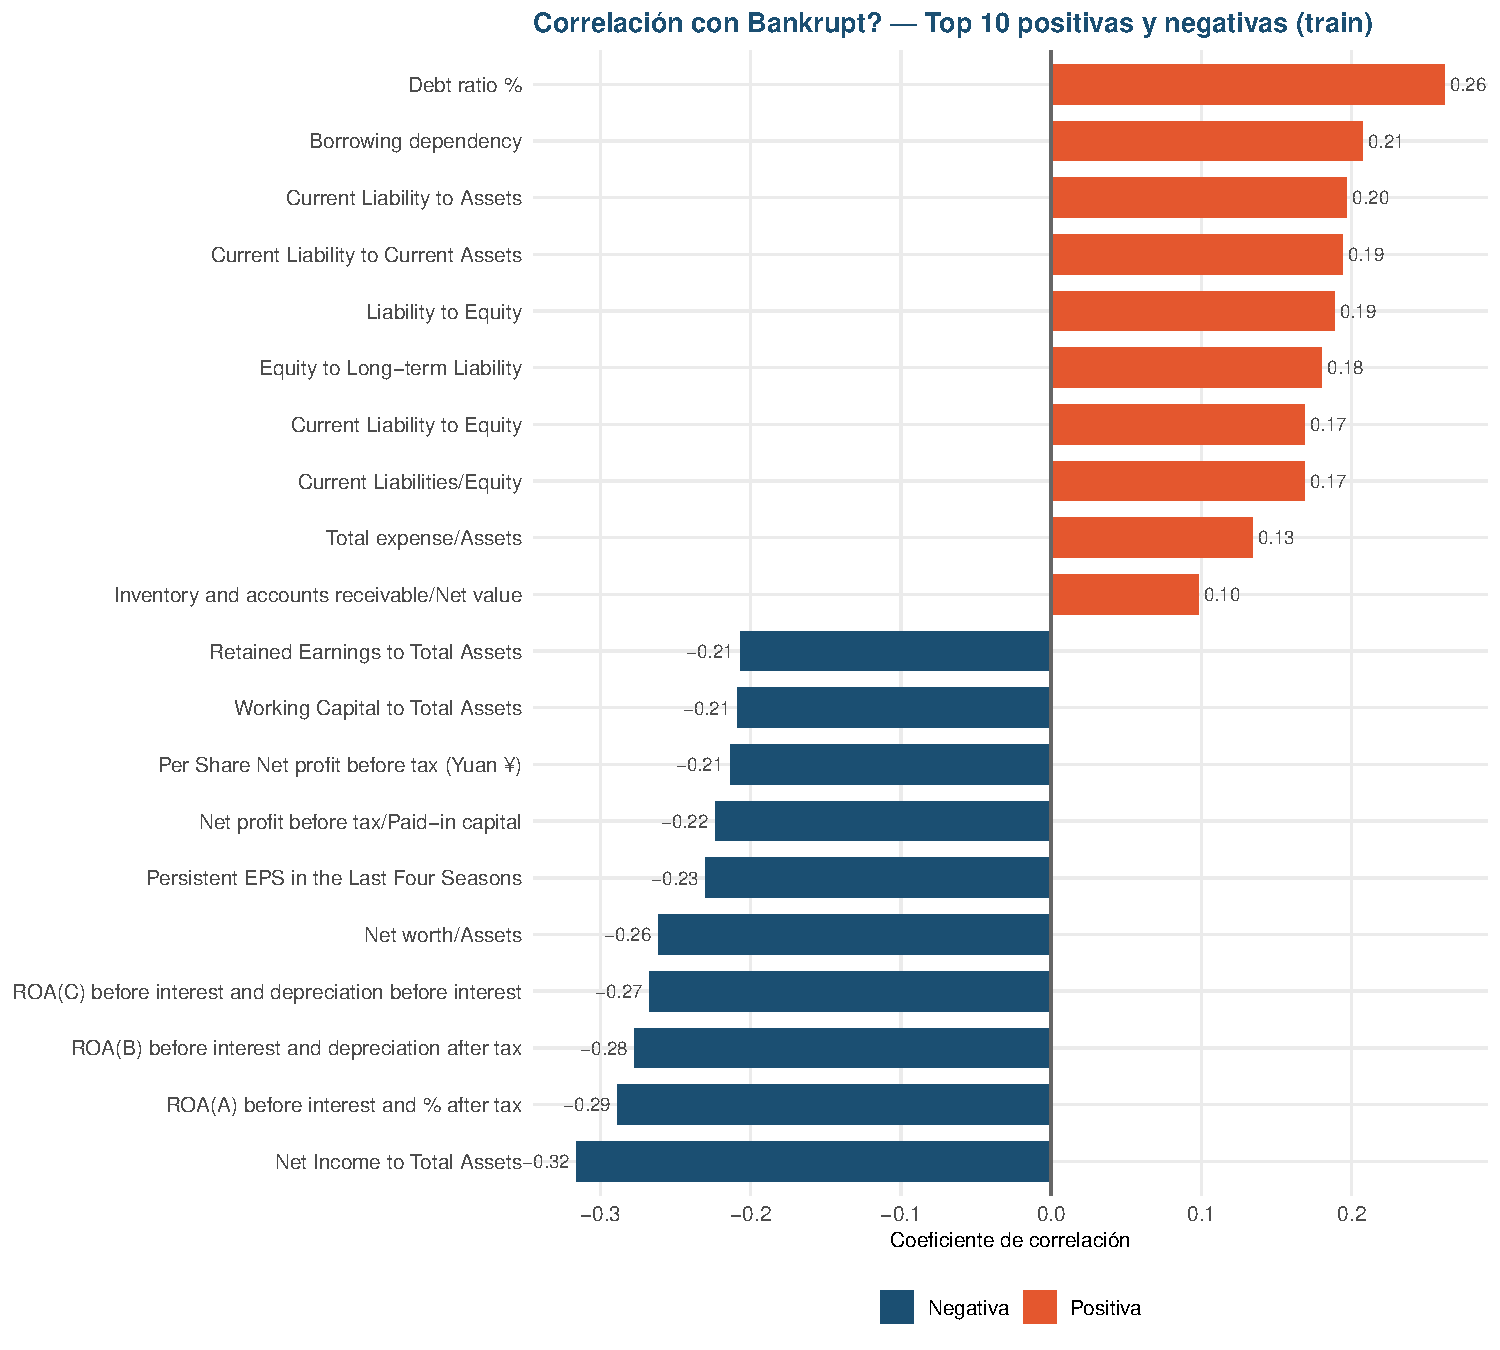
\includegraphics[keepaspectratio]{Prediccion_Bancarrota_Empresarial_files/Prediccion_Bancarrota_Empresarial_files/figure-latex/correlaciones-1.pdf}}

\textbf{En palabras simples:} el gráfico confirma, con números, lo que ya insinuaba el
Random Forest: \textbf{rentabilidad y endeudamiento son los dos bloques que más se
relacionan con la quiebra}, pero en direcciones opuestas.

\begin{itemize}
\tightlist
\item
  \textbf{Correlaciones negativas (azul):} dominadas por variables de \textbf{rentabilidad} ---
  distintas versiones de ROA, utilidad neta sobre activos/patrimonio, ganancias
  retenidas. La relación es negativa porque tiene sentido financiero: \textbf{a mayor
  rentabilidad, menor probabilidad de quiebra}.
\item
  \textbf{Correlaciones positivas (naranja):} dominadas por variables de
  \textbf{endeudamiento} --- \texttt{Debt\ ratio\ \%}, \texttt{Borrowing\ dependency}, varias razones de
  pasivos sobre activos o patrimonio. Aquí la relación es positiva porque \textbf{a mayor
  nivel de deuda relativa, mayor probabilidad de quiebra}.
\end{itemize}

Es importante notar que ninguna correlación individual suele superar \textasciitilde0.32 en valor
absoluto: son relaciones reales pero moderadas, no fuertes. Esto refuerza una
conclusión que ya se venía formando en el EDA: ninguna variable por sí sola explica
bien la quiebra, por lo que un modelo que combine varias señales (como Random Forest)
probablemente capture mejor el patrón que basarse en una sola razón financiera.

También vale la pena notar que varias de las variables con correlación negativa más
fuerte (las distintas versiones de ROA) son las mismas que ya se identifican como
altamente correlacionadas entre sí en la siguiente sección de multicolinealidad --- otra
razón para tenerlas presentes al momento de seleccionar variables para el modelo.

\section{Matriz de correlación de las variables más importantes}\label{matriz-de-correlaciuxf3n-de-las-variables-muxe1s-importantes}

\begin{Shaded}
\begin{Highlighting}[]
\NormalTok{corr\_features }\OtherTok{\textless{}{-}} \FunctionTok{c}\NormalTok{(top\_15\_features, TARGET)}
\NormalTok{corr\_matrix   }\OtherTok{\textless{}{-}} \FunctionTok{cor}\NormalTok{(train\_df[corr\_features], }\AttributeTok{use =} \StringTok{"pairwise.complete.obs"}\NormalTok{)}

\FunctionTok{ggcorrplot}\NormalTok{(}
\NormalTok{  corr\_matrix, }\AttributeTok{lab =} \ConstantTok{TRUE}\NormalTok{, }\AttributeTok{lab\_size =} \FloatTok{2.8}\NormalTok{, }\AttributeTok{type =} \StringTok{"full"}\NormalTok{,}
  \AttributeTok{colors =} \FunctionTok{c}\NormalTok{(COLOR\_MAIN, }\StringTok{"white"}\NormalTok{, COLOR\_RISK),}
  \AttributeTok{outline.color =} \StringTok{"white"}\NormalTok{,}
  \AttributeTok{title =} \StringTok{"Matriz de correlación — Top 15 variables (train)"}
\NormalTok{) }\SpecialCharTok{+}
  \FunctionTok{theme}\NormalTok{(}
    \AttributeTok{plot.title =} \FunctionTok{element\_text}\NormalTok{(}\AttributeTok{face =} \StringTok{"bold"}\NormalTok{, }\AttributeTok{size =} \DecValTok{15}\NormalTok{, }\AttributeTok{color =}\NormalTok{ COLOR\_MAIN),}
    \AttributeTok{axis.text.x =} \FunctionTok{element\_text}\NormalTok{(}\AttributeTok{angle =} \DecValTok{45}\NormalTok{, }\AttributeTok{hjust =} \DecValTok{1}\NormalTok{, }\AttributeTok{size =} \DecValTok{8}\NormalTok{),}
    \AttributeTok{axis.text.y =} \FunctionTok{element\_text}\NormalTok{(}\AttributeTok{size =} \DecValTok{8}\NormalTok{)}
\NormalTok{  )}
\end{Highlighting}
\end{Shaded}

\pandocbounded{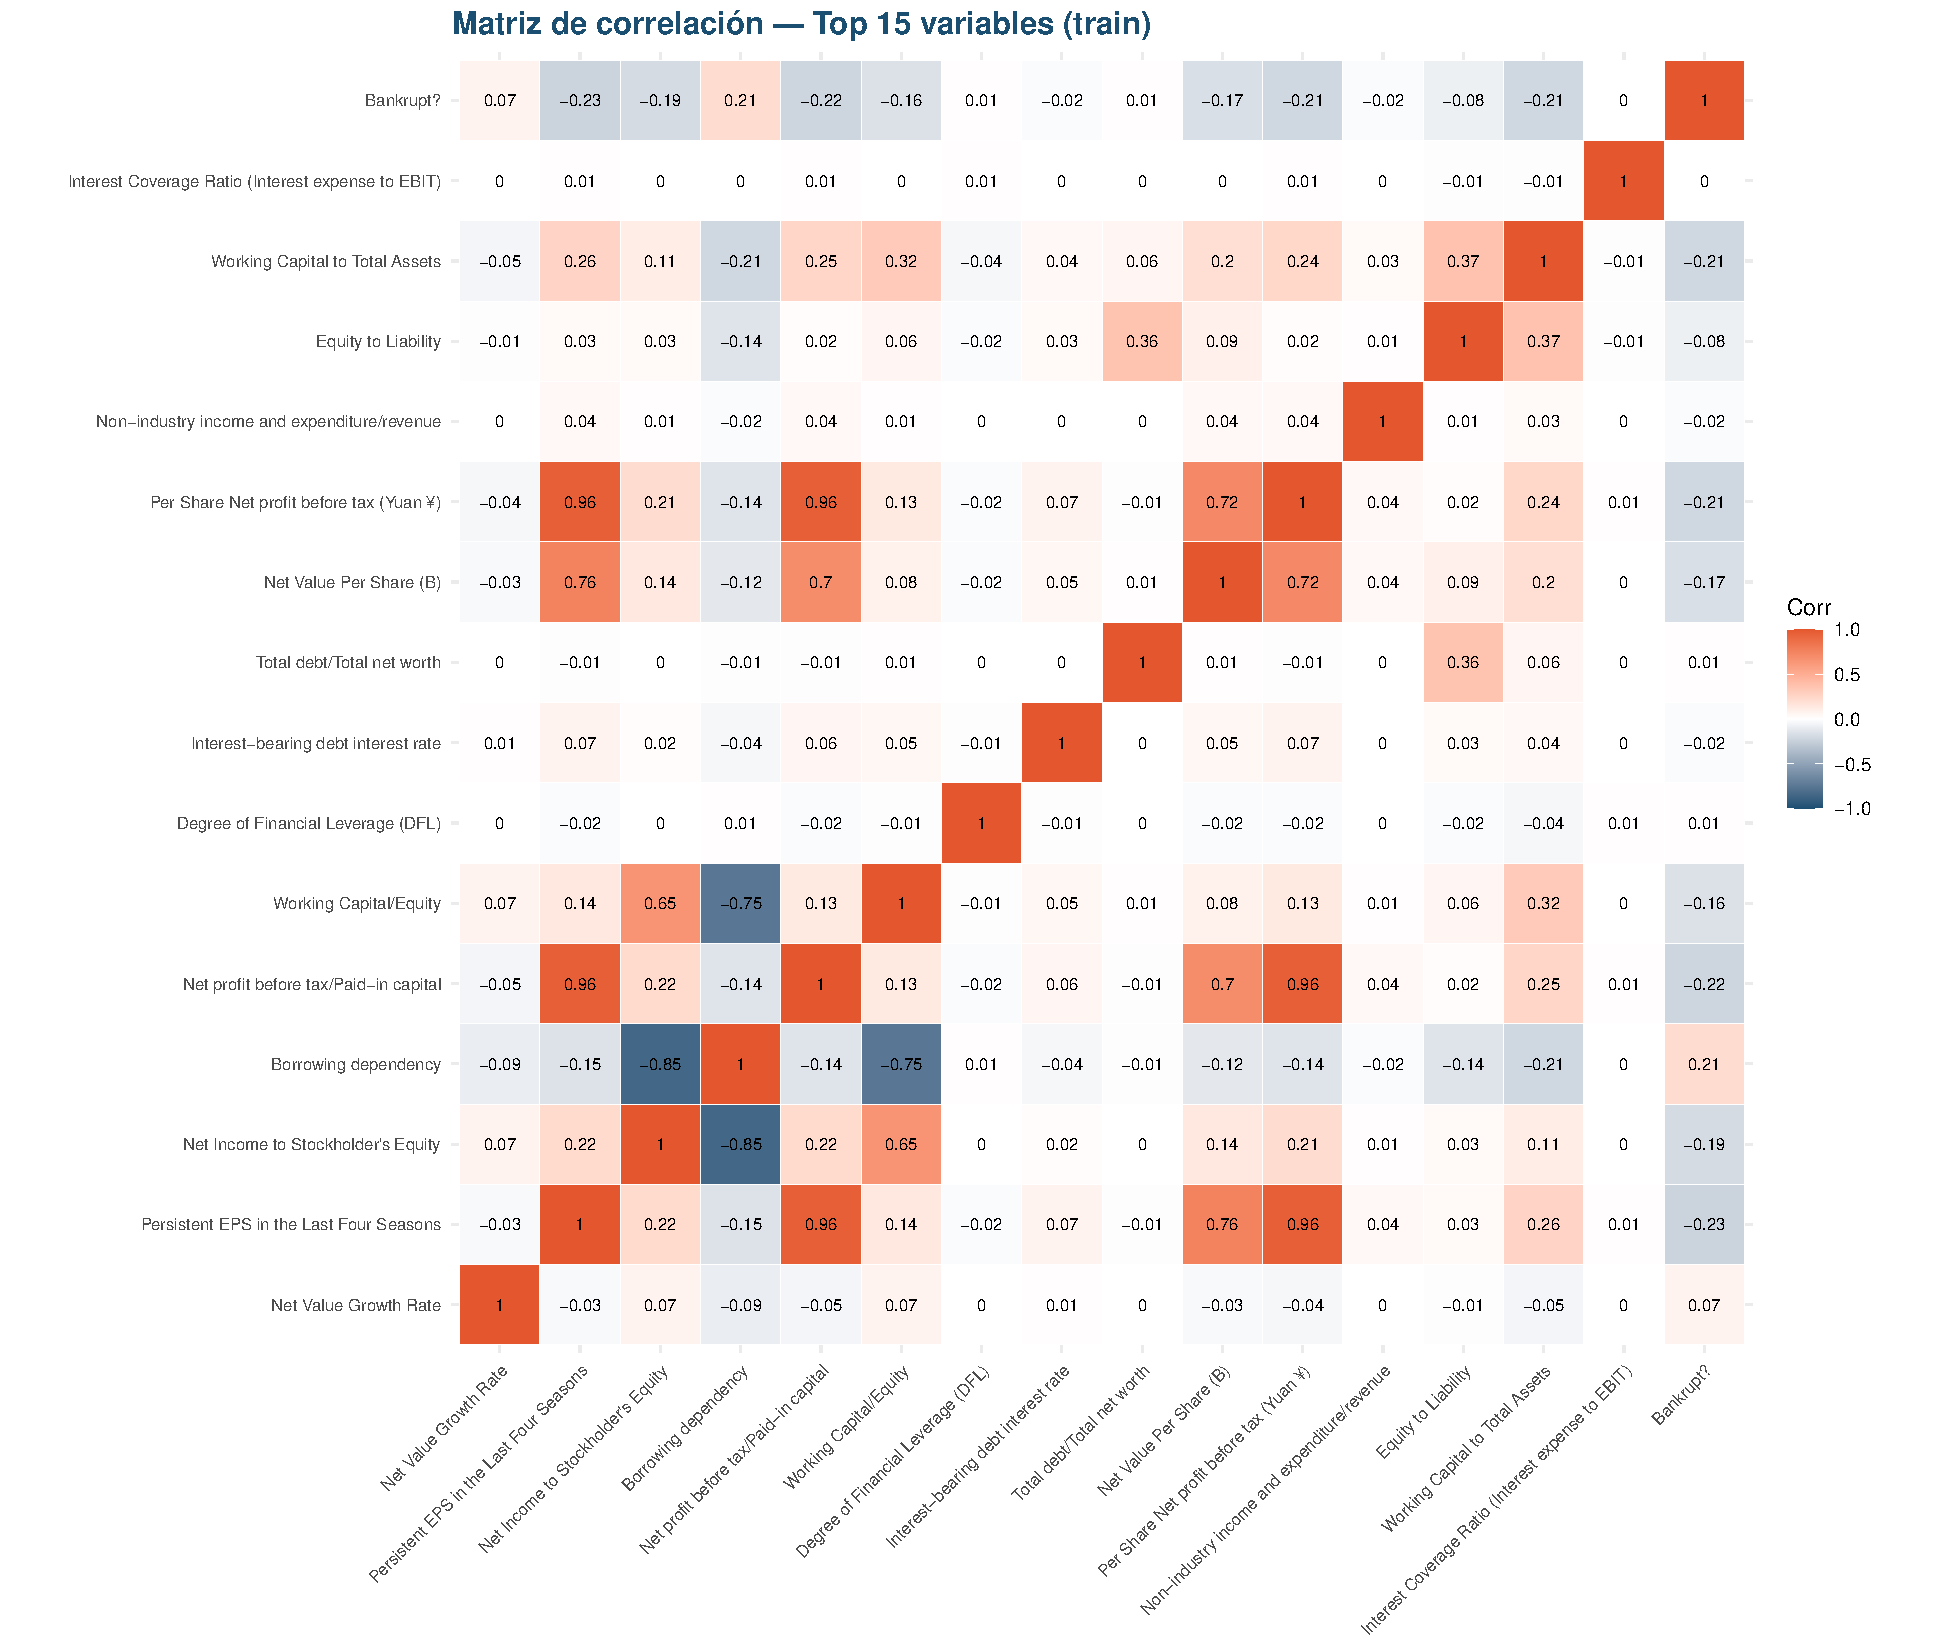
\includegraphics[keepaspectratio]{Prediccion_Bancarrota_Empresarial_files/Prediccion_Bancarrota_Empresarial_files/figure-latex/heatmap-corr-1.pdf}}

Esta matriz reúne en un solo lugar las 15 variables más relevantes según Random
Forest, junto con \texttt{Bankrupt?}, para ver cómo se relacionan entre sí (no solo con la
quiebra).

\begin{itemize}
\tightlist
\item
  \textbf{Última fila/columna (\texttt{Bankrupt?}):} muestra correlaciones moderadas con las demás
  variables, consistentes con lo visto arriba --- ninguna supera \textasciitilde0.3 en valor absoluto,
  lo que confirma que ninguna variable por sí sola explica la quiebra con fuerza.
\item
  \textbf{Bloques oscuros entre variables (no con el target):} aquí está lo más llamativo.
  Varias combinaciones de ROA, utilidad neta y ganancias retenidas muestran
  correlaciones muy altas entre sí (cercanas a 0.9-1.0). Esto confirma la
  \textbf{multicolinealidad}: son distintas formas de medir prácticamente lo mismo
  (rentabilidad), calculadas con pequeñas variaciones metodológicas.
\end{itemize}

Esto no afecta a Random Forest (que ya usamos para identificar estas variables), pero
si más adelante se prueba un modelo lineal (como regresión logística), meter varias
versiones casi idénticas del mismo ratio no aporta información nueva y puede inflar
artificialmente la importancia de esa ``familia'' de variables o dificultar la
interpretación de los coeficientes. Por ahora no se elimina ninguna --- esa decisión se
deja para la etapa de preprocesamiento, con más contexto sobre qué modelo se va a
usar.

\chapter{Conclusiones del EDA}\label{conclusiones-del-eda}

\begin{enumerate}
\def\labelenumi{\arabic{enumi}.}
\item
  \textbf{Estructura del dataset:} \texttt{train} tiene alrededor de 5.455 empresas y 95
  variables predictoras (93 numéricas + 2 flags binarios), más el target
  \texttt{Bankrupt?}.
\item
  \textbf{Calidad de los datos:} no hay valores nulos ni filas duplicadas en \texttt{train}, lo
  cual facilita el modelado. \texttt{Net\ Income\ Flag} es (casi) constante y no aporta
  información --- candidata a eliminarse.
\item
  \textbf{Desbalance del target:} el problema es de clasificación binaria con un
  desbalance fuerte (aproximadamente 20-30 empresas sanas por cada empresa
  quebrada). Esto obliga a usar métricas distintas al accuracy y a considerar
  técnicas de balanceo en el modelado, no en el EDA.
\item
  \textbf{Sesgo y outliers:} varias variables financieras tienen sesgo alto y un
  porcentaje considerable de outliers según IQR. No parecen errores de captura, sino
  comportamientos extremos reales de algunas empresas, por lo que su tratamiento
  (transformación, winsorizing, o dejarlos igual) debe decidirse con cuidado más
  adelante.
\item
  \textbf{Variables relevantes:} según Random Forest y correlación con el target, las
  variables de \textbf{rentabilidad} (ROA, utilidad neta sobre patrimonio) y de
  \textbf{endeudamiento} son las que más distinguen a las empresas que quiebran de las
  que no.
\item
  \textbf{Multicolinealidad:} existen varias versiones muy parecidas del mismo indicador
  (por ejemplo, distintas formas de calcular ROA), altamente correlacionadas entre
  sí. No se eliminó ninguna en esta etapa, pero es algo a tener en cuenta si se usa
  un modelo lineal.
\item
  \textbf{\texttt{Liability-Assets\ Flag}:} tiene muy pocos casos con valor 1, pero ese grupo
  pequeño concentra una proporción de quiebra más alta. Vale la pena conservarla
  para el modelo pese a su baja cardinalidad.
\end{enumerate}

\section{Problemas identificados para la etapa de preprocesamiento}\label{problemas-identificados-para-la-etapa-de-preprocesamiento}

\begin{itemize}
\tightlist
\item
  \textbf{\texttt{Net\ Income\ Flag}} es (casi) constante en todo el dataset: evaluar si eliminarla
  antes de entrenar el modelo.
\item
  \textbf{Escalas muy distintas entre variables:} será necesario estandarizar/normalizar
  dentro del pipeline (ajustando el escalador solo con \texttt{train} y aplicándolo después
  a \texttt{test} --- por ejemplo con \texttt{caret::preProcess()}).
\item
  \textbf{Variables con sesgo alto y muchos outliers:} decidir si se transforman (por
  ejemplo, con logaritmo), se recortan (winsorizing) o se dejan igual, y documentar la
  razón.
\item
  \textbf{Multicolinealidad entre variantes de ROA y otros indicadores:} considerar
  selección de variables (\texttt{caret::findCorrelation()}) o técnicas de regularización si
  se usa un modelo lineal.
\item
  \textbf{Desbalance de clases (\textasciitilde3\% quebradas):} aplicar técnicas de balanceo (por
  ejemplo, \texttt{class\ weights} en \texttt{randomForest}, o sobre/submuestreo con paquetes como
  \texttt{ROSE} o \texttt{smotefamily}) solo sobre \texttt{train}, y elegir métricas de evaluación
  adecuadas para clases desbalanceadas (recall, F1, AUC-PR) en lugar de accuracy.
\item
  \textbf{\texttt{Liability-Assets\ Flag} con muy pocos casos positivos:} vigilar que la partición
  train/test (ya estratificada por el target) no deje casos demasiado escasos de este
  flag en algún fold si más adelante se usa validación cruzada
  (\texttt{caret::createFolds()}).
\end{itemize}

\bibliography{book.bib}

\end{document}
